% =================================================================
% Guía de programación PLC con Arduino Opta — Guía del estudiante
% Autora: María del Milagro Rojas Sánchez
% Formato: article, una columna, español — misma identidad tipográfica
% que Documento_TFG.tex (12pt, márgenes, interlineado, encabezado).
% =================================================================
\documentclass[12pt,a4paper]{article}

% -------------------------------------------------
% Paquetes
% -------------------------------------------------
\usepackage[utf8]{inputenc}
\usepackage[T1]{fontenc}
\usepackage[spanish,es-nodecimaldot,es-noquoting]{babel}
\usepackage{graphicx}
\graphicspath{{./}{imagenes/}{../imagenes/}{../Guia_FluidSIM_OPTA_LadderSecuencial/imgs/}}
\usepackage{cite}
\usepackage{booktabs}
\usepackage{tabularx}
\usepackage{array}
\usepackage{xcolor}
\usepackage{listings}
\usepackage[most]{tcolorbox}
\usepackage{amsmath}
\usepackage{tikz}
\usetikzlibrary{positioning,arrows.meta}
\usepackage{float}
\usepackage{geometry}
\usepackage{fancyhdr}
\usepackage{titlesec}
\usepackage{tocloft}
\usepackage[hidelinks]{hyperref}
\usepackage{xurl}

% babel-spanish impone `Cuadro''; se fuerza `Tabla'', como en el informe.
\AtBeginDocument{\renewcommand{\tablename}{Tabla}\renewcommand{\listtablename}{Índice de tablas}}

% El rótulo "Apéndice A/B/C" (ver \appendix más abajo) es más ancho que el
% número "1." de una sección normal; sin ensanchar esta columna del índice,
% el título del apéndice se superpone con su propio número.
\setlength{\cftsecnumwidth}{9em}

% -------------------------------------------------
% Márgenes y espaciado — igual que Documento_TFG.tex, para que ambos
% documentos se lean como parte del mismo proyecto.
% -------------------------------------------------
\geometry{a4paper, left=3cm, right=2.5cm, top=3cm, bottom=3cm}
\linespread{1.25}
\setlength{\parskip}{6pt}
\setlength{\parindent}{0.75cm}
\setcounter{secnumdepth}{4}

% -------------------------------------------------
% Colores — misma paleta que el informe y la presentación
% -------------------------------------------------
\definecolor{DeepBlue}{HTML}{16324F}
\definecolor{SoftBlue}{HTML}{EAF2FB}
\definecolor{SoftGray}{HTML}{F3F5F7}

% Locales de este documento (no forman parte de la paleta de identidad
% compartida): solo para la caja de Precaución, a pedido de la autora.
\definecolor{DarkRed}{HTML}{8B1E1E}
\definecolor{SoftRed}{HTML}{FBE7E7}

% Locales: muestras del color físico de cada hilo del cable SysLink
% (sección del EasyPort). Codifican el color real del cable, no la
% identidad visual del documento — igual que los Wire* de la tarjeta de
% cableado.
\definecolor{HiloBlanco}{HTML}{FFFFFF}
\definecolor{HiloMarron}{HTML}{7B4A2A}
\definecolor{HiloVerde}{HTML}{2E8B3A}
\definecolor{HiloAmarillo}{HTML}{F2C80F}
\definecolor{HiloGris}{HTML}{9A9A9A}
\definecolor{HiloRosa}{HTML}{F4A6C0}
\definecolor{HiloAzul}{HTML}{2B5DB8}
\definecolor{HiloRojo}{HTML}{C62828}
\definecolor{HiloNegro}{HTML}{111111}
\definecolor{HiloPurpura}{HTML}{7B3FA0}
\definecolor{HiloNaranja}{HTML}{F28C28}
\definecolor{HiloCeleste}{HTML}{6EC6F0}

% \hilo{A}{B}: muestra de un hilo bicolor (A/B); \hilo{A}{A} para un solo color.
\newcommand{\hilo}[2]{\tikz[baseline=-0.1ex]{%
    \fill[#1] (0,-0.35ex) rectangle (0.7em,1.25ex);
    \fill[#2] (0.7em,-0.35ex) rectangle (1.4em,1.25ex);
    \draw[black!60, line width=0.3pt] (0,-0.35ex) rectangle (1.4em,1.25ex);}}

% -------------------------------------------------
% Encabezado y pie de página
% -------------------------------------------------
\pagestyle{fancy}
\fancyhf{}
\fancyhead[L]{\small\textcolor{DeepBlue}{Guía de práctica estudiantil para PLC con Arduino Opta}}
\fancyhead[R]{\small María del Milagro Rojas Sánchez}
\fancyfoot[C]{\thepage}
\renewcommand{\headrulewidth}{0.4pt}

% -------------------------------------------------
% Estilo de los títulos de sección — color de la paleta, sin recargar
% -------------------------------------------------
\titleformat{\section}{\normalfont\Large\bfseries\color{DeepBlue}}{\thesection.}{0.6em}{}
\titlespacing*{\section}{0pt}{1.6em}{0.8em}
\titleformat{\subsection}{\normalfont\large\bfseries\color{DeepBlue}}{\thesubsection}{0.6em}{}
\titlespacing*{\subsection}{0pt}{1.3em}{0.6em}
\titleformat{\subsubsection}{\normalfont\normalsize\bfseries\color{DeepBlue}}{\thesubsubsection}{0.6em}{}
\titlespacing*{\subsubsection}{0pt}{1.1em}{0.5em}
\titleformat{\paragraph}[block]{\normalfont\normalsize\bfseries\color{DeepBlue}}{\theparagraph}{0.6em}{}
\titlespacing*{\paragraph}{0pt}{1em}{0.4em}

% -------------------------------------------------
% Macros de interfaz
% La aplicación está en inglés: todo elemento de la interfaz se
% escribe con su nombre literal en inglés usando estas macros.
% -------------------------------------------------
% \ui{Watch}            -> un control, ventana o botón
% \menu{Project}{Options} -> una ruta de menú
% \key{F7}              -> una tecla o atajo
\newcommand{\ui}[1]{\textcolor{DeepBlue}{\textsf{\textbf{#1}}}}
\newcommand{\menu}[2]{\textcolor{DeepBlue}{\textsf{\textbf{#1}\,$\rightarrow$\,\textbf{#2}}}}
\newcommand{\key}[1]{\textcolor{DeepBlue}{\textsf{\small\fbox{#1}}}}

% Marcador temporal de contenido pendiente
\newcommand{\pendiente}[1]{\textcolor{red}{\textbf{[PENDIENTE: #1]}}}

% -------------------------------------------------
% Cajas de nota, advertencia y práctica
% -------------------------------------------------
\newtcolorbox{nota}[1][]{
    colback=SoftBlue, colframe=DeepBlue, boxrule=0.6pt, arc=2pt,
    left=6pt, right=6pt, top=5pt, bottom=5pt,
    fonttitle=\bfseries\sffamily\small, title=Nota, #1}

\newtcolorbox{advertencia}[1][]{
    colback=SoftRed, colframe=DarkRed, boxrule=0.6pt, arc=2pt,
    left=6pt, right=6pt, top=5pt, bottom=5pt,
    fonttitle=\bfseries\sffamily\small, title=Precaución, #1}

\newtcolorbox{practica}[2][]{
    colback=SoftBlue, colframe=DeepBlue, boxrule=0.8pt, arc=2pt,
    left=6pt, right=6pt, top=5pt, bottom=5pt,
    fonttitle=\bfseries\sffamily, title=Práctica: #2, #1}

% -------------------------------------------------
% Estilo para listados de Structured Text
% -------------------------------------------------
\lstdefinelanguage{ST}{
    morekeywords={PROGRAM,END_PROGRAM,FUNCTION,END_FUNCTION,
        FUNCTION_BLOCK,END_FUNCTION_BLOCK,VAR,VAR_INPUT,VAR_OUTPUT,
        VAR_IN_OUT,VAR_GLOBAL,END_VAR,IF,THEN,ELSIF,ELSE,END_IF,
        CASE,OF,END_CASE,FOR,TO,BY,DO,END_FOR,WHILE,END_WHILE,
        REPEAT,UNTIL,END_REPEAT,EXIT,RETURN,TRUE,FALSE,AND,OR,XOR,NOT,
        BOOL,INT,DINT,UINT,UDINT,REAL,LREAL,WORD,DWORD,BYTE,TIME,STRING},
    sensitive=false,
    morecomment=[s]{(*}{*)},
    morecomment=[l]{//},
    morestring=[b]'
}

\lstset{
    language=ST,
    basicstyle=\ttfamily\footnotesize,
    keywordstyle=\color{DeepBlue}\bfseries,
    commentstyle=\color{DeepBlue}\itshape,
    stringstyle=\color{orange!80!black},
    backgroundcolor=\color{SoftGray},
    frame=leftline,
    rulecolor=\color{DeepBlue},
    framesep=6pt,
    xleftmargin=10pt,
    numbers=left,
    numberstyle=\ttfamily\scriptsize\color{gray},
    numbersep=8pt,
    breaklines=true,
    showstringspaces=false,
    captionpos=b
}

% =================================================================
\begin{document}
% =================================================================

% -------------------------------------------------
% Portada estilo TEC
% -------------------------------------------------
\begin{titlepage}
    \thispagestyle{empty}
    \begin{center}

        \vspace*{1cm}
        
\includegraphics[width=0.6\textwidth]{logo_tec.png}

        \vspace{2cm}

        {\large Campus Tecnológico San Carlos}\\[0.3cm]
        {\large Escuela de Ingeniería en Electrónica}\\[0.3cm]
        {\large Curso: Proyecto Final de Graduación}\\[0.3cm]
        {\large Profesor Asesor: Ing. Pablo César Rodríguez Vargas}\\[0.3cm]
        {\large Grupo: 50}\\[0.3cm]

        \vspace{2cm}

        {\Large \textbf{GUÍA DE PRÁCTICA ESTUDIANTIL PARA PLC}}\\[0.3cm]
        {\large Arduino OPTA IDE}

        \vspace{2cm}

        {\large Elaborado por:}\\[0.2cm]
        {\large María del Milagro Rojas Sánchez}

        \vfill

        {\large San Carlos -- Alajuela -- Costa Rica}\\[0.2cm]
        {\large Año 2026.}

    \end{center}
\end{titlepage}

% -------------------------------------------------
% Resumen e índice
% -------------------------------------------------
\begin{abstract}
Esta guía introduce la programación de controladores lógicos programables (PLC)
sobre la plataforma didáctica basada en Arduino Opta, empleando el entorno
Arduino PLC IDE. Se abordan tres de los cinco lenguajes definidos por la norma
IEC~61131-3: Structured Text (ST), Ladder Diagram (LD) y Function Block Diagram
(FBD). El documento está dirigido a estudiantes de la Escuela de Ingeniería
Electrónica que utilizarán el gabinete de control del laboratorio, y combina la
explicación de cada lenguaje con prácticas verificables sobre el hardware
disponible (los módulos DIN Simul8 y DIN Celsius, y la expansión de señales
analógicas) y sobre el software de simulación FluidSIM, enlazado con el
Opta real para las prácticas que lo requieren.
\end{abstract}

\medskip
\noindent\textbf{Palabras clave:} PLC, IEC 61131-3, Arduino Opta, Ladder
Diagram, Structured Text, Function Block Diagram, FluidSIM, automatización
industrial.

\tableofcontents
\bigskip\hrule\bigskip

% =================================================================
\section{Prácticas de laboratorio}
% =================================================================

Cada práctica de esta guía abre con un recuadro que resume su objetivo,
los materiales y programas necesarios y el montaje (físico, virtual o
ambos); a continuación se desarrolla el procedimiento paso a paso. La Práctica~1 se
describe con el mayor detalle posible porque es, para la mayoría de los
estudiantes, el primer contacto simultáneo con tres cosas nuevas: el
lenguaje Ladder Diagram, el software FluidSIM y el Arduino Opta real. Las
prácticas siguientes podrán ser más breves y remitir a esta cuando repitan
un procedimiento ya explicado aquí.

\begin{table}[H]
\centering
\caption{Hardware disponible para las prácticas. Fuente: Autora.}
\label{tab:hardware}
\renewcommand{\arraystretch}{1.4}
\begin{tabularx}{\linewidth}{l X}
\toprule
\textbf{Módulo} & \textbf{Uso previsto en las prácticas} \\
\midrule
Arduino Opta WiFi     & Controlador; entradas y salidas propias. \\
DIN Simul8            & Ocho interruptores como entradas digitales y
                        distribución de 24~V. \\
DIN Celsius           & Dos calentadores y un sensor de temperatura
                        ($-10$ a $125\,^\circ$C) para lazos de control. \\
Opta Ext A0602 (AFX00007) & Expansión de entradas y salidas analógicas. \\
EasyPort USB (D16A)   & Interfaz entre FluidSIM y el panel: lleva por
                        cable real las señales del proceso simulado
                        (sección~\ref{subsec:easyport}). \\
\bottomrule
\end{tabularx}
\end{table}

\subsection{Tutoriales oficiales de Arduino}
\label{sec:tutoriales_arduino}

Antes de la primera práctica conviene revisar dos tutoriales oficiales que
Arduino ofrece como guía básica introductoria para el uso del PLC IDE. Son
material propio de Arduino, no de esta guía, y se referencian aquí como
punto de partida complementario, no como sustituto de las prácticas:

\begin{itemize}
    \item \textit{Programming Introduction with Arduino PLC
    IDE}~\cite{plcintro}: recorre la creación de un proyecto y presenta
    los cinco lenguajes de la norma IEC~61131-3 con ejemplos sencillos. Es
    la referencia oficial para Structured Text, Function Block Diagram,
    Instruction List y Sequential Function Chart: los lenguajes que esta
    guía no desarrolla en detalle, ya que todas las prácticas propias de
    esta guía están hechas íntegramente en Ladder Diagram.\\
    \url{https://docs.arduino.cc/software/plc-ide/tutorials/plc-programming-introduction/}
    \item \textit{Opta Analog Expansion Usage with the PLC
    IDE}~\cite{optaanalogtut}: muestra cómo configurar y leer o escribir
    el módulo de expansión analógica del Opta (AFX00007) desde el PLC IDE.\\
    \url{https://docs.arduino.cc/software/plc-ide/tutorials/opta-analog-expansion-plc-ide/}
\end{itemize}

% -------------------------------------------------
\subsection{Introducción a FluidSIM}
\label{subsec:intro_fluidsim}

Un PLC solo cobra sentido cuando tiene algo que controlar: cilindros que
avanzan, motores que arrancan, sensores que detectan una pieza. El panel del
laboratorio trae pulsadores, luces y relés, pero no una línea de producción
completa. Para eso está FluidSIM, el software de Festo Didactic para diseñar
y simular circuitos neumáticos, hidráulicos y eléctricos~\cite{fluidsim}. En
FluidSIM se dibuja la ``planta'' (la máquina o proceso que el PLC va a
gobernar) y, al iniciar la simulación, esa planta cobra vida en pantalla:
los cilindros se desplazan, las lámparas se encienden y los manómetros marcan
presión, todo en tiempo real.

\subsubsection{Qué permite hacer}
\begin{itemize}
    \item Dibujar circuitos con símbolos normalizados, arrastrándolos desde
    una biblioteca y uniéndolos con el ratón.
    \item Simular y animar el circuito: ver qué se mueve, qué se energiza y
    en qué orden, y accionar pulsadores con un clic mientras corre.
    \item Equivocarse sin consecuencias: un cable mal conectado en FluidSIM no
    quema nada, así que los errores se encuentran antes de tocar el hardware.
    \item Conectar el circuito a un controlador externo. En esta guía ese
    controlador es el Arduino Opta: FluidSIM hace de máquina y el Opta, de
    cerebro (sección~\ref{subsec:easyport}).
\end{itemize}

\subsubsection{La biblioteca de componentes}
Todo lo que se puede colocar en un circuito sale de la ventana
\ui{Biblioteca} (figura~\ref{fig:fs_biblioteca}). Tres detalles de esta
ventana ahorran tiempo:

\begin{itemize}
    \item La pestaña \ui{Símbolos estándar} lleva un candado: es la
    biblioteca de fábrica y no se modifica, solo se toman componentes de ella.
    \item El buscador encuentra un componente por su nombre sin recorrer las
    carpetas; con \ui{Búsqueda por similitud} activada basta escribir parte de
    la palabra (por ejemplo, ``cilindro'' o ``temporizador''), y
    \ui{Palabra completa} restringe a coincidencias exactas.
    \item El número de la esquina indica cuántos símbolos hay disponibles
    (873 en la instalación del laboratorio).
\end{itemize}

\begin{figure}[!t]
    \centering
    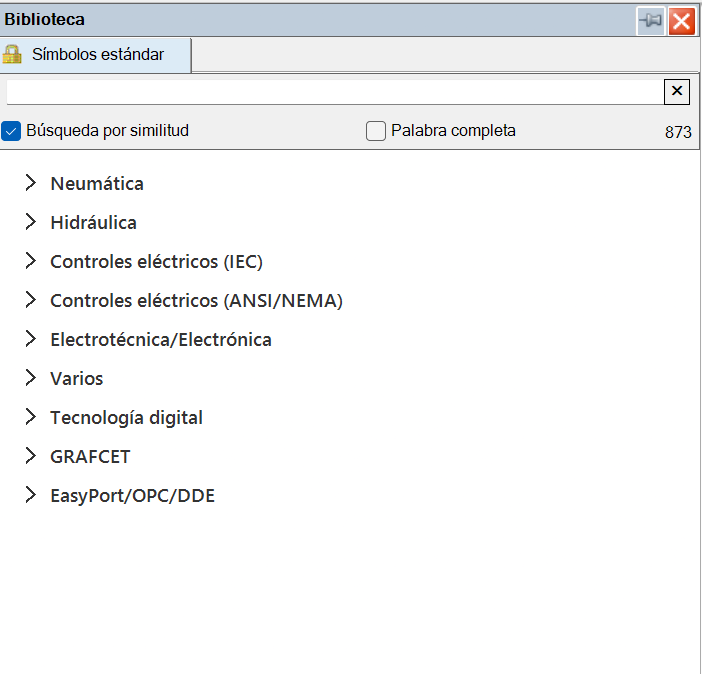
\includegraphics[width=0.6\linewidth]{Biblioteca_FluidSIM.png}
    \caption{Ventana \ui{Biblioteca} de FluidSIM con sus nueve categorías.}
    \label{fig:fs_biblioteca}
\end{figure}

Los componentes se agrupan en nueve categorías. La
tabla~\ref{tab:fs_categorias} resume qué contiene cada una y qué parte de una
instalación industrial permite recrear~\cite{fluidsimlib}.

\begin{table}[!htbp]
\centering
\caption{Categorías de la biblioteca de FluidSIM. Fuente: Autora.}
\label{tab:fs_categorias}
\linespread{1}\small\selectfont
\renewcommand{\arraystretch}{1.3}
\begin{tabularx}{\linewidth}{>{\raggedright\arraybackslash}p{3.4cm} X X}
\toprule
\textbf{Categoría} & \textbf{Qué contiene} & \textbf{Qué permite recrear} \\
\midrule
Neumática &
Fuente de aire comprimido, unidad de mantenimiento, válvulas
distribuidoras (3/2, 5/2) de accionamiento manual, mecánico o eléctrico,
reguladores de caudal y presión, cilindros, pinzas, ventosas de vacío. &
Prensas, sujeción y expulsión de piezas, manipuladores
\textit{pick and place}, líneas de empaque. \\
Hidráulica &
Grupo hidráulico (bomba y depósito), válvulas direccionales, de presión y
de caudal, cilindros, motores hidráulicos, manómetros. &
Equipos de mucha fuerza: prensas pesadas, elevadores, maquinaria móvil. \\
Controles eléctricos (IEC) &
Fuente de 24~V, pulsadores, interruptores, finales de carrera, sensores de
proximidad, relés y contactores, relés temporizados, lámparas, bobinas de
electroválvula. &
El circuito de mando: lo que el operario acciona, lo que detecta la
máquina y lo que se enciende o se energiza. \\
Controles eléctricos (ANSI/NEMA) &
Los mismos elementos de mando, con la simbología norteamericana. &
Planos de mando con estilo estadounidense. \\
Electrotécnica/ Electrónica &
Fuentes, resistencias, condensadores, semiconductores, motores, máquinas
eléctricas, instrumentos de medida. &
Circuitos de potencia y medición: arranque de un motor, consumo de una
carga. \\
Varios &
Elementos auxiliares de dibujo y documentación. &
Rotular y presentar el circuito. \\
Tecnología digital &
Constantes, compuertas lógicas (AND, OR, NOT), biestables, contadores y
funciones especiales. &
Lógica cableada o de un relé programable sencillo, sin PLC externo. \\
GRAFCET &
Etapas, transiciones y acciones. &
La secuencia de una máquina, dibujada paso a paso antes de programarla. \\
EasyPort/ OPC/DDE &
Bloques de entrada y salida, digitales y analógicos, hacia el exterior
de FluidSIM. &
El enlace con un controlador real: aquí la planta virtual se conecta al
Opta. \\
\bottomrule
\end{tabularx}
\end{table}

\begin{nota}
Las dos categorías de controles eléctricos contienen lo mismo con distinta
simbología. Esta guía usa la de IEC, la norma europea e internacional que
también rige la programación del PLC (IEC~61131-3). Conviene elegir una sola
y no mezclar símbolos de ambas en un mismo circuito.
\end{nota}

\subsubsection{Cómo se arma una planta virtual}
Casi cualquier máquina automatizada se modela en FluidSIM con tres capas,
que conviene construir en este orden:

\begin{enumerate}
    \item Potencia: lo que realiza el trabajo físico. Cilindros, válvulas y
    su alimentación de aire o aceite (categorías Neumática o Hidráulica), o
    motores (Electrotécnica).
    \item Mando eléctrico: pulsadores, sensores, relés y bobinas de
    electroválvula a 24~V (Controles eléctricos IEC). Es el puente entre la
    potencia y el controlador.
    \item Controlador: quien decide. Puede resolverse dentro del propio
    FluidSIM (relés, Tecnología digital, GRAFCET), pero en esta guía esa
    decisión la toma el programa Ladder del Opta, al que se llega por los
    bloques de la categoría EasyPort/OPC/DDE.
\end{enumerate}

La Práctica~1 sigue exactamente este esquema: cuatro cilindros con sus
electroválvulas (potencia), dos pulsadores y cuatro relés (mando) y el Opta
como controlador.

\begin{nota}
GRAFCET es una herramienta útil antes de escribir Ladder: dibujar la
secuencia como etapas y transiciones obliga a decidir qué ocurre en cada paso
y qué condición permite avanzar al siguiente. Una vez claro el GRAFCET,
traducirlo a Ladder es casi mecánico.
\end{nota}

% -------------------------------------------------
\subsection{Conexión con el EasyPort}
\label{subsec:easyport}

\subsubsection{Qué es el EasyPort}
El EasyPort USB (modelo D16A) de Festo Didactic es una interfaz de
proceso: un traductor entre el computador y el mundo de los 24~V
industriales~\cite{easyport}. Por un lado se conecta al PC por USB; por el
otro ofrece bornes de señal reales. Cuando un bloque de FluidSIM pone un bit
en 1, el EasyPort entrega 24~V en el pin correspondiente; cuando recibe 24~V
en una de sus entradas, FluidSIM ve ese bit en 1. Así, la planta virtual y el
Opta intercambian señales por cables reales, igual que lo harían una máquina
y su PLC en una fábrica (figura~\ref{fig:easyport_cadena}).

\begin{figure}[!t]
    \centering
    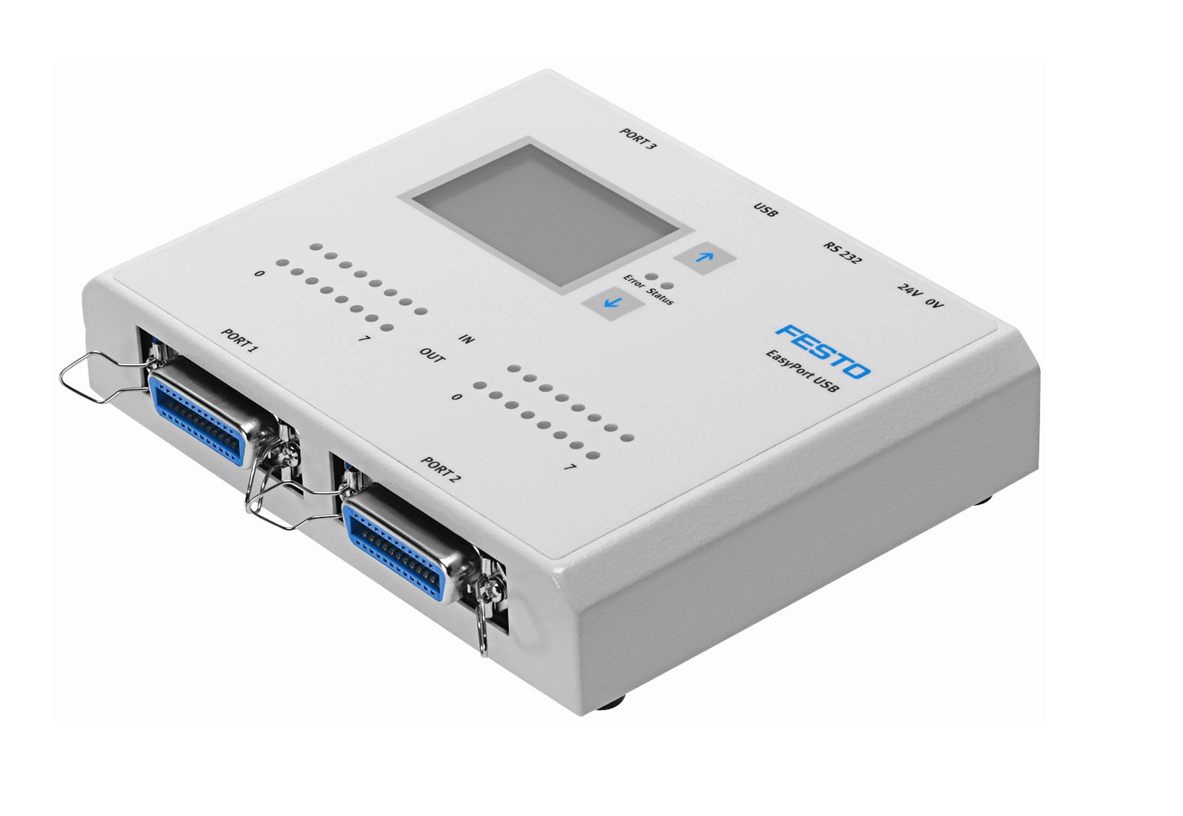
\includegraphics[width=0.55\linewidth]{EasyPort_perfil.png}
    \caption{EasyPort USB (D16A): puertos SysLink digitales 1 y 2 y puerto
    analógico 3.}
    \label{fig:easyport}
\end{figure}

Sus datos principales~\cite{easyport}:

\begin{itemize}
    \item 16 entradas y 16 salidas digitales de 24~V, repartidas en dos
    puertos SysLink (Port~1 y Port~2) de 8 entradas y 8 salidas cada uno.
    Cada salida entrega hasta 0,7~A y está protegida contra cortocircuito;
    una entrada se lee como 1 a partir de unos 12~V.
    \item 4 entradas y 2 salidas analógicas (0--10~V o $\pm$10~V, 12 bits) en
    el Port~3, un conector Sub-D de 15 pines.
    \item Alimentación externa de 24~V~DC ($\pm$10~\%), por los bornes de la
    parte trasera o por los puertos SysLink.
    \item LEDs de estado por canal: verdes para las entradas y amarillos para
    las salidas. Un LED rojo de error indica un cortocircuito en alguna
    salida; en ese caso el EasyPort desactiva sus salidas.
\end{itemize}

% [H]: el diagrama se queda aquí, después de la lista; flotando partía en
% dos el párrafo siguiente.
\begin{figure}[H]
\vspace{1.2em}
\centering
\begin{tikzpicture}[
    bloque/.style={draw=DeepBlue, fill=SoftBlue, thick, rounded corners=2pt,
                   align=center, minimum width=2.7cm, minimum height=1.7cm,
                   font=\normalsize},
    flecha/.style={-{Stealth[length=2.2mm]}, thick, DeepBlue},
    etiqueta/.style={font=\footnotesize, align=center}]
    \node[bloque] (fs) {FluidSIM\\[-1pt]{\scriptsize planta virtual (PC)}};
    \node[bloque, right=1.4cm of fs] (ep) {EasyPort USB\\[-1pt]{\scriptsize D16A}};
    \node[bloque, right=5.2cm of ep] (opta) {Arduino Opta\\[-1pt]{\scriptsize bornes del panel}};
    \draw[{Stealth[length=2.2mm]}-{Stealth[length=2.2mm]}, thick, DeepBlue]
        (fs) -- node[etiqueta, above] {USB} (ep);
    \draw[flecha] ([yshift=5mm]ep.east) -- node[etiqueta, above]
        {salidas EasyPort (pines 1--8)\\$\rightarrow$ entradas del Opta}
        ([yshift=5mm]opta.west);
    \draw[flecha] ([yshift=-5mm]opta.west) -- node[etiqueta, below]
        {salidas del Opta\\$\rightarrow$ entradas EasyPort (pines 13--20)}
        ([yshift=-5mm]ep.east);
\end{tikzpicture}
\caption{Cadena de señales: los sensores y pulsadores virtuales llegan a las
entradas del Opta, y las salidas del Opta mueven los actuadores virtuales. El
tramo EasyPort--Opta es el cable SysLink. Fuente: Elaborado con IA diagram.}
\label{fig:easyport_cadena}
\end{figure}

\subsubsection{El EasyPort dentro de FluidSIM}
\label{subsubsec:fs_easyport}
En la biblioteca, la categoría EasyPort/OPC/DDE
(figura~\ref{fig:fs_biblioteca}) reúne los bloques que comunican el circuito
con el exterior: \ui{FluidSIM In} y \ui{FluidSIM Out} para señales
digitales, sus equivalentes analógicos y un distribuidor de
conector~\cite{fluidsimlib} (figuras~\ref{fig:fs_in} y~\ref{fig:fs_out}).
OPC y DDE son enlaces por software con otros programas; para el EasyPort
interesan los bloques digitales.

\begin{figure}[!t]
    \centering
    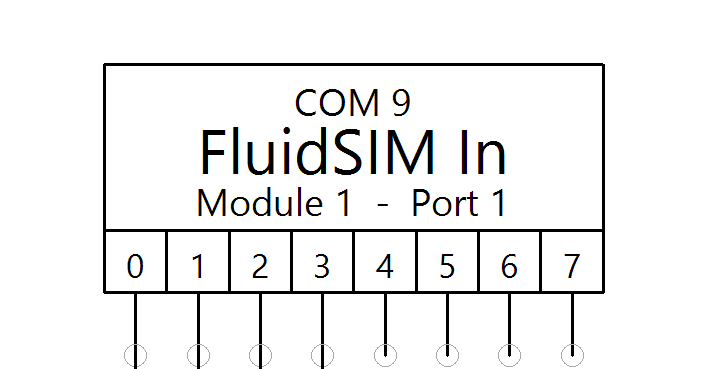
\includegraphics[width=0.7\linewidth]{03_fluidsim_in.png}
    \caption{Bloque \ui{FluidSIM In}.}
    \label{fig:fs_in}
\end{figure}

\begin{figure}[!t]
    \centering
    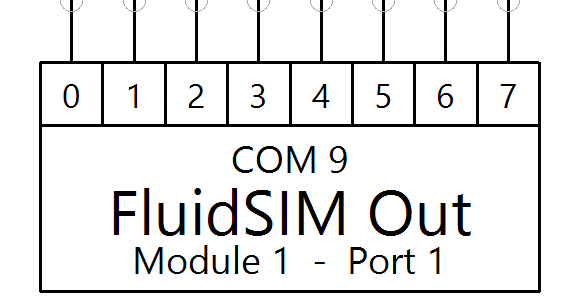
\includegraphics[width=0.7\linewidth]{04_fluidsim_out.png}
    \caption{Bloque \ui{FluidSIM Out}.}
    \label{fig:fs_out}
\end{figure}

\paragraph{Cómo se leen los nombres In/Out}
\label{par:fs_inout}
Los nombres \ui{In}/\ui{Out} se leen desde el punto de vista de FluidSIM,
y es la fuente de la mayoría de las confusiones al usarlos por primera vez:
\begin{itemize}
    \item \ui{FluidSIM In} trae al circuito lo que llega a las entradas del
    EasyPort. Cuando una entrada del EasyPort recibe 24~V (por ejemplo,
    desde una salida de relé del Opta), el canal correspondiente del
    bloque pone un 1 lógico en el circuito y puede energizar, por ejemplo,
    la bobina de un relé.
    \item \ui{FluidSIM Out} lleva hacia afuera el estado de un punto del
    circuito: cuando ese punto está en 24~V, la salida correspondiente del
    EasyPort entrega 24~V reales en su borne, suficientes para encender una
    luz LED de 24~V.
\end{itemize}

\begin{advertencia}
Todo lo que llega desde afuera hacia la planta virtual (las salidas del
Opta) se conecta al bloque \ui{FluidSIM In}. Todo lo que la planta virtual
debe mostrar o enviar afuera (las luces LED del panel) sale por el bloque
\ui{FluidSIM Out}.
\end{advertencia}

Cada bloque representa un puerto de 8 bits del EasyPort, y en sus
propiedades se indican tres datos, que el propio bloque muestra en su
rótulo (por ejemplo, \texttt{COM~9}, \texttt{Module~1 - Port~1}):

\begin{itemize}
    \item \ui{Interfaz serie}: el puerto COM que Windows asigna al EasyPort
    al conectarlo por USB.
    \item \ui{Número de puerto}: el conector SysLink que se usa, 1 o 2.
    \item \ui{Módulo}: la dirección del EasyPort, de 1 a 4. Viene de fábrica
    en 1 y solo cambia si se conectan varios EasyPort al mismo PC.
\end{itemize}

El paso a paso para configurarlos está en la
sección~\ref{subsubsec:puesta_marcha}.

Los canales 0 a 7 del bloque corresponden a los bits 0 a 7 de ese puerto,
es decir, a los hilos de la tabla~\ref{tab:syslink}.

\subsubsection{El cable de E/S SysLink}
El EasyPort se une al panel con un cable de E/S que tiene, en un extremo, el
conector SysLink de 24 pines (norma IEEE~488) y, en el otro, 21 hilos sueltos
de 0,34~mm$^2$ con puntera (figura~\ref{fig:cable_syslink})~\cite{syslinkcable}.
Un cable lleva las 16 señales de un puerto (8 bits de salida y 8 de
entrada), además de la alimentación. En el conector, los pines 9--10,
21--22 y 23--24 están puenteados; por eso el cable trae menos hilos que
pines.

\begin{figure}[!t]
    \centering
    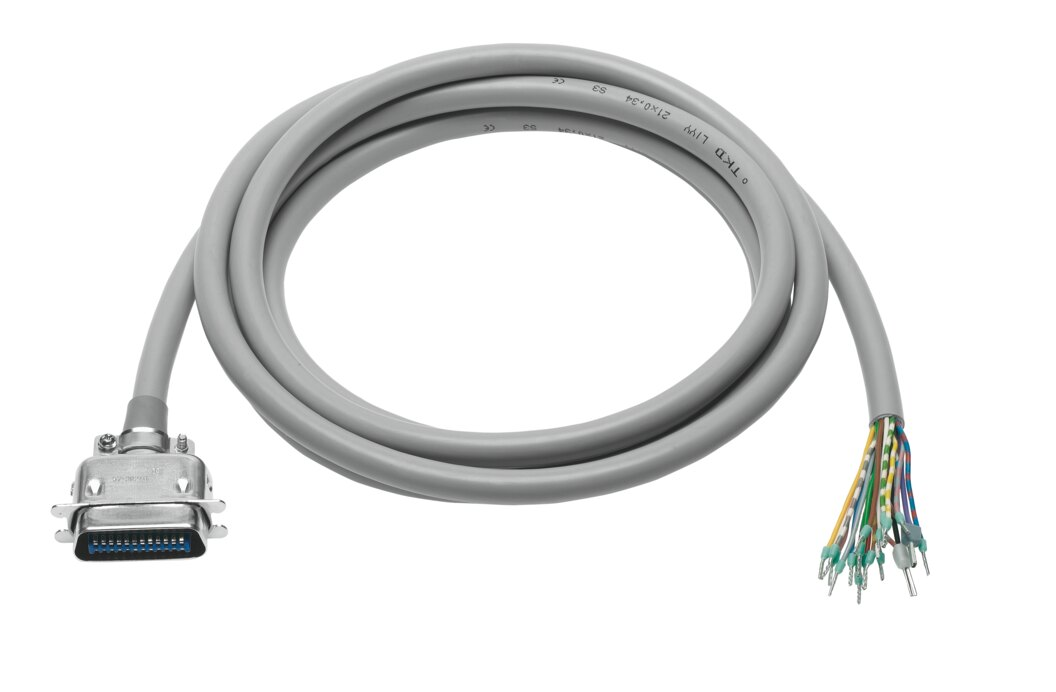
\includegraphics[width=0.6\linewidth]{Cable_Perfil_Easyport.jpg}
    \caption{Cable de E/S con conector SysLink y terminales abiertos.
    Fuente: Festo~\cite{syslinkweb}.}
    \label{fig:cable_syslink}
\end{figure}

La tabla~\ref{tab:syslink} reorganiza la asignación de pines del fabricante
según la función de cada hilo: salidas del EasyPort, entradas del EasyPort y
alimentación. El borne del panel al que va cada hilo se indica en cada
práctica.

\begin{table}[!htbp]
\centering
\caption{Cable SysLink: pines y colores de los hilos. Asignación de
pines y colores según~\cite{syslinkcable}.}
\label{tab:syslink}
\linespread{1}\small\selectfont
\renewcommand{\arraystretch}{1.15}
\begin{tabularx}{\linewidth}{c X X}
\toprule
\textbf{Pin} & \textbf{Señal del EasyPort} & \textbf{Color del hilo} \\
\midrule
\multicolumn{3}{l}{\textit{Salidas del EasyPort $\rightarrow$ entradas del
Opta (sensores y pulsadores de FluidSIM)}} \\
\midrule
1 & Output bit 0 & \hilo{HiloBlanco}{HiloBlanco}~Blanco \\
2 & Output bit 1 & \hilo{HiloMarron}{HiloMarron}~Marrón \\
3 & Output bit 2 & \hilo{HiloVerde}{HiloVerde}~Verde \\
4 & Output bit 3 & \hilo{HiloAmarillo}{HiloAmarillo}~Amarillo \\
5 & Output bit 4 & \hilo{HiloGris}{HiloGris}~Gris \\
6 & Output bit 5 & \hilo{HiloRosa}{HiloRosa}~Rosa \\
7 & Output bit 6 & \hilo{HiloAzul}{HiloAzul}~Azul \\
8 & Output bit 7 & \hilo{HiloRojo}{HiloRojo}~Rojo \\
\midrule
\multicolumn{3}{l}{\textit{Salidas del Opta $\rightarrow$ entradas del
EasyPort (actuadores de FluidSIM)}} \\
\midrule
13 & Input bit 0 & \hilo{HiloGris}{HiloRosa}~Gris/rosa \\
14 & Input bit 1 & \hilo{HiloRojo}{HiloAzul}~Rojo/azul \\
15 & Input bit 2 & \hilo{HiloBlanco}{HiloVerde}~Blanco/verde \\
16 & Input bit 3 & \hilo{HiloMarron}{HiloVerde}~Marrón/verde \\
17 & Input bit 4 & \hilo{HiloBlanco}{HiloAmarillo}~Blanco/amarillo \\
18 & Input bit 5 & \hilo{HiloAmarillo}{HiloMarron}~Amarillo/marrón \\
19 & Input bit 6 & \hilo{HiloBlanco}{HiloGris}~Blanco/gris \\
20 & Input bit 7 & \hilo{HiloGris}{HiloMarron}~Gris/marrón \\
\midrule
\multicolumn{3}{l}{\textit{Alimentación}} \\
\midrule
11 & 0~V & \hilo{HiloRosa}{HiloMarron}~Rosa/marrón \\
12 & 0~V & \hilo{HiloPurpura}{HiloPurpura}~Púrpura \\
23 & 0~V & \hilo{HiloBlanco}{HiloAzul}~Blanco/azul \\
9  & 24~V & \hilo{HiloNegro}{HiloNegro}~Negro \\
21 & 24~V & \hilo{HiloBlanco}{HiloRosa}~Blanco/rosa \\
\bottomrule
\end{tabularx}
\end{table}

\begin{advertencia}
Antes de conectar, con todo apagado:
\begin{itemize}
    \item El EasyPort se alimenta por un solo lado~\cite{easyport}. En el
    panel se alimenta por sus bornes traseros de 24~V, así que los hilos de
    24~V del cable (negro y blanco/rosa) no se conectan a ninguna fuente:
    se aíslan.
    \item El 0~V sí se comparte. Un hilo de 0~V del cable va al 0~V común del
    panel; sin esa referencia común, el Opta y el EasyPort no ``ven'' los
    24~V del otro.
    \item Los relés del Opta son contactos secos: no generan tensión. Para que
    el NA entregue 24~V a la entrada del EasyPort, el común de cada relé debe
    estar unido a +24~V.
    \item Una salida del EasyPort nunca se une a otra fuente ni a otra
    salida. Si se enciende el LED rojo de error, hay un cortocircuito.
    \item Las puntas de los hilos libres se aíslan para que no toquen ningún
    borne.
\end{itemize}
\end{advertencia}

\subsubsection{El cable analógico}
\label{subsubsec:cable_analogico}
Las señales analógicas no viajan por SysLink: el Port~3 del EasyPort es un
conector Sub-D de 15 pines con 4 entradas y 2 salidas de 0 a
10~V~\cite{easyport}. El cable usado en el panel tiene un hilo de color por
cada pin útil (tabla~\ref{tab:cable_analogico}); los pines 4, 5, 9, 10, 12
y 13 no se usan. Como en el cable SysLink, el borne del panel al que va
cada hilo se indica en cada práctica.

Los números de canal de la tabla son los que muestra la pantalla del
EasyPort. El programa Festo EasyPort Web Bridge numera las entradas desde
1: el canal~0 de la pantalla aparece allí como \ui{Uin 1}.

\begin{table}[H]
\centering
\caption{Cable analógico del Port~3: pines, colores de los hilos y canal
que muestra el EasyPort. Pines según~\cite{easyport}; colores y canales
medidos en el banco. Fuente: Autora.}
\label{tab:cable_analogico}
\linespread{1}\small\selectfont
\renewcommand{\arraystretch}{1.15}
\begin{tabularx}{\linewidth}{c X X}
\toprule
\textbf{Pin} & \textbf{Señal del EasyPort} & \textbf{Color del hilo} \\
\midrule
\multicolumn{3}{l}{\textit{Entradas analógicas (0--10~V hacia el EasyPort)}} \\
\midrule
8  & Entrada, canal~0 & \hilo{HiloAmarillo}{HiloAmarillo}~Amarillo \\
7  & Entrada, canal~1 & \hilo{HiloCeleste}{HiloCeleste}~Celeste \\
15 & Entrada, canal~2 & \hilo{HiloMarron}{HiloMarron}~Café \\
14 & Entrada, canal~3 & \hilo{HiloBlanco}{HiloBlanco}~Blanco \\
\midrule
\multicolumn{3}{l}{\textit{Salidas analógicas (0--10~V desde el EasyPort)}} \\
\midrule
1  & Salida~0 & \hilo{HiloNaranja}{HiloNaranja}~Naranja \\
2  & Salida~1 & \hilo{HiloVerde}{HiloVerde}~Verde \\
\midrule
\multicolumn{3}{l}{\textit{Referencias}} \\
\midrule
3  & 0~V & \hilo{HiloNegro}{HiloNegro}~Negro \\
6  & 0~V & \hilo{HiloGris}{HiloGris}~Gris \\
11 & +10~V de referencia & \hilo{HiloRojo}{HiloRojo}~Rojo \\
\bottomrule
\end{tabularx}
\end{table}

\subsubsection{Orden de puesta en marcha}
\label{subsubsec:puesta_marcha}
\begin{enumerate}
    \item Cablear con todo apagado, según las conexiones que indique la
    práctica y los colores de las tablas~\ref{tab:syslink} (digital)
    y~\ref{tab:cable_analogico} (analógico).
    \item Encender la fuente de 24~V del panel.
    \item Conectar el EasyPort al PC por USB. El LED verde de estado
    parpadea a 1~Hz mientras espera comunicación.
    \item En FluidSIM, configurar cada bloque \ui{FluidSIM In} y
    \ui{FluidSIM Out} del circuito. Con doble clic sobre el bloque se abre su
    ventana de propiedades (figura~\ref{fig:conf_puerto_easy}); en ella:
    \begin{enumerate}
        \item En \ui{Conectar EasyPort mediante}, seleccionar
        \ui{Conexión directa EasyPort}.
        \item En la pestaña \ui{COM}, campo \ui{Interfaz serie}, seleccionar
        el puerto COM en el que está conectado el USB del EasyPort.
        \item Verificar que \ui{Número de puerto} y \ui{Módulo} coincidan con
        lo que indique la práctica.
        \item Hacer clic en \ui{Aceptar}.
    \end{enumerate}
    \begin{figure}[H]
        \centering
        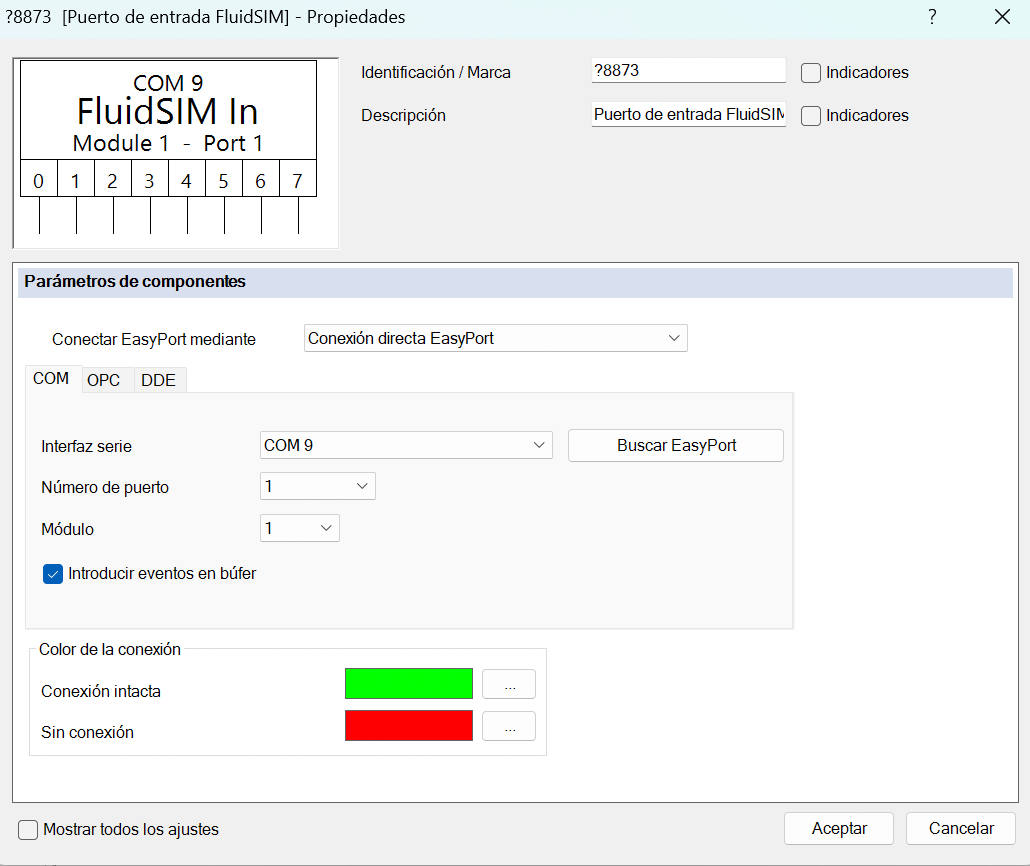
\includegraphics[width=0.62\linewidth]{Conf_Puerto_Easy.png}
        \caption{Propiedades de un bloque \ui{FluidSIM In}: conexión directa
        al EasyPort por el puerto \texttt{COM~9}, puerto 1, módulo 1.}
        \label{fig:conf_puerto_easy}
    \end{figure}
    \item Iniciar la simulación. Cuando FluidSIM se comunica con el EasyPort,
    el LED de estado cambia a un parpadeo pulsante.
\end{enumerate}

\begin{nota}
Para saber qué puerto COM usa el EasyPort, abrir el \ui{Administrador de
dispositivos} de Windows y desplegar \ui{Puertos (COM y LPT)}. Si hay varios,
desconectar y volver a conectar el USB del EasyPort: el puerto que desaparece
y reaparece es el suyo. El número puede cambiar si se usa otro puerto USB del
computador, así que conviene revisarlo en cada sesión.
\end{nota}

\subsection[Práctica 1: secuencia de 5 estados]{Práctica 1: secuencia de 5 estados con Ladder, FluidSIM y el Arduino Opta}
\label{subsec:practica1}

\begin{practica}{Secuencia de 5 estados}
\textbf{Objetivo.} Automatizar un proceso secuencial como los que se
encuentran en una línea de producción: una estación que activa cuatro
actuadores uno tras otro, en un orden y con unos tiempos fijos. El proceso
se programa en Ladder Diagram como una máquina de cinco estados y el
operador lo gobierna, como en cualquier máquina industrial, con dos
pulsadores sin enclavamiento: el pulsador~1 da la señal de inicio de la
secuencia y el pulsador~2 es la condición de parada.\\
\textbf{Materiales.} Plataforma didáctica de PLC, cuatro luces indicadoras
LED de 24~V, dos pulsadores sin enclavamiento de 24~V, EasyPort USB con su
cable SysLink, cable USB-C, computador con PLC IDE y FluidSIM
instalados.\\
\textbf{Montaje.} Mixto, físico y virtual. Los dos pulsadores se cablean
a entradas del PLC de la plataforma; las salidas de relé \texttt{O1} a
\texttt{O4} van al EasyPort, que las lleva a FluidSIM, y las cuatro luces
LED se conectan a las salidas del EasyPort. FluidSIM simula la parte
neumática de la estación (sección~\ref{subsec:easyport}). Así, el estudiante acciona la máquina con
sus manos y ve cada estado a la vez en la pantalla y en el panel.\\
\textbf{Flujo.} Primero se escribe y se descarga el programa Ladder en el
Opta (secciones~\ref{subsubsec:p1_programa}
a~\ref{subsubsec:p1_ladder}); después se arma la planta en FluidSIM y se
cablea el enlace con el Opta (sección~\ref{subsubsec:p1_fluidsim}).
\end{practica}

\subsubsection{Descripción del ejercicio}

Dos pulsadores sin enclavamiento (momentáneos: activos solo mientras se
mantienen presionados) controlan una secuencia de cuatro ``cilindros'',
representados por cuatro LEDs o salidas de relé:

\begin{itemize}
    \item \textbf{Pulsador 1 (arranque):} normalmente abierto (NA). Al
    presionarlo una vez, arranca la secuencia.
    \item \textbf{Pulsador 2 (parada):} actúa como permiso de marcha.
    Mientras no se presiona, permite el funcionamiento; al presionarlo,
    corta todo de inmediato.
\end{itemize}

La secuencia recorre cinco estados:

\begin{enumerate}
    \item \textbf{Reposo:} ningún LED encendido, a la espera del
    pulsador~1.
    \item Se activa \texttt{Led1} de inmediato al presionar el pulsador~1.
    \item A los 5~s, se activa \texttt{Led2}, sin apagar \texttt{Led1}.
    \item A los 5~s siguientes (10~s desde el arranque), se activa
    \texttt{Led3}.
    \item A los 5~s siguientes (15~s desde el arranque), se activa
    \texttt{Led4}. Los cuatro permanecen encendidos hasta que se presiona el
    pulsador~2, momento en el que se apagan y el sistema queda listo para un
    nuevo arranque.
\end{enumerate}

Toda la lógica de secuencia y temporización vive en el Arduino Opta,
programado en Ladder. FluidSIM solo simula la parte ``de campo''
(cilindros, válvulas y relés) y se comunica con el Opta real a través del
EasyPort y su cable SysLink.

% -------------------------------------------------
\subsubsection{Creación del programa Ladder}
\label{subsubsec:p1_programa}

Se parte de un proyecto nuevo para el Opta, creado como se muestra en el
tutorial introductorio de Arduino (sección~\ref{sec:tutoriales_arduino}).
Ese proyecto trae por defecto un programa principal (\texttt{main}) en
Structured Text; el ejercicio se escribe en un programa aparte, en Ladder:

\begin{enumerate}
    \item En el árbol del proyecto, hacer clic derecho sobre el nombre del
    proyecto (el nodo raíz) y elegir \menu{New object}{New program}. Si la
    opción aparece deshabilitada, es porque no se seleccionó primero el nodo
    raíz.
    \item En la ventana \ui{New program} (figura~\ref{fig:crear_programa}),
    marcar \ui{LD} en \ui{Language} y escribir el nombre del programa en
    \ui{Name}; en este ejercicio, \texttt{Ejercicio1\_\allowbreak Señales\_\allowbreak Digitales}.
    \item Hacer clic en \ui{OK}. El programa se abre con una red
    (\emph{rung}) vacía.
\end{enumerate}

\begin{figure}[H]
    \centering
    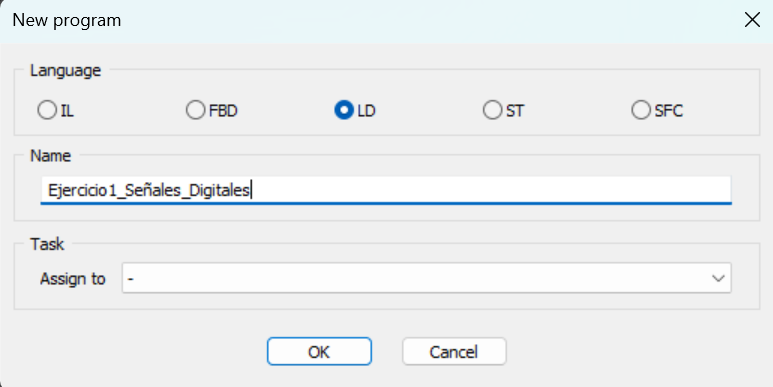
\includegraphics[width=0.7\linewidth]{Crear_programa_ejercicio1.png}
    \caption{Ventana \ui{New program}: lenguaje \ui{LD} y nombre del
    programa.}
    \label{fig:crear_programa}
\end{figure}

\begin{advertencia}
Crear el programa LD no basta: hay que asignarlo a una tarea de ejecución
para que el runtime lo ejecute; de lo contrario compila sin errores pero
nunca corre. Puede hacerse en esta misma ventana, con el campo
\ui{Assign to} de \ui{Task}, o después, en \menu{Project}{Tasks} $\to$
\ui{Fast} (doble clic), agregando el programa a la lista de POUs de esa
tarea.
\end{advertencia}

% -------------------------------------------------
\subsubsection{Mapeo de entradas y salidas}
\label{subsubsec:p1_mapeo}

Antes de dibujar las redes se da nombre a los canales físicos del Opta que
usa el programa, en las tablas del nodo \ui{Local I/O Mapping}.

\paragraph{Entradas}
Con doble clic en \menu{Local I/O Mapping}{Programmable Inputs} se abre la
tabla de mapeo de entradas (figura~\ref{fig:plcide_inputs}). En la columna
\ui{Variable} se escriben los nombres de la tabla~\ref{tab:mapeo_entradas}:
\texttt{Start} en \texttt{I1}, para el pulsador~1 (inicio de la
secuencia), y \texttt{Run} en \texttt{I2}, para el pulsador~2 (condición de
parada). El IDE completa por sí solo el tipo (\texttt{BOOL}).

\begin{figure}[H]
    \centering
    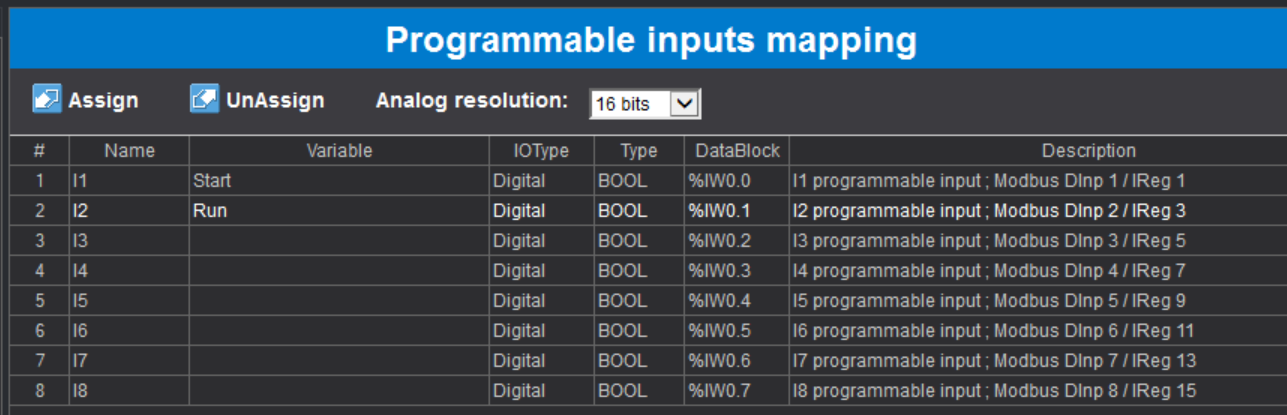
\includegraphics[width=0.9\linewidth]{08_programmable_inputs_mapping.png}
    \caption{Mapeo de entradas programables: \texttt{Start} en \texttt{I1}
    y \texttt{Run} en \texttt{I2}.}
    \label{fig:plcide_inputs}
\end{figure}

\begin{table}[!t]
\centering
\caption{Mapeo de entradas usado en este ejercicio. Fuente: Autora.}
\label{tab:mapeo_entradas}
\renewcommand{\arraystretch}{1.4}
\begin{tabularx}{\linewidth}{l l X}
\toprule
\textbf{Canal} & \textbf{Variable} & \textbf{Significado} \\
\midrule
I1 & \texttt{Start} & Pulsador~1, inicio de la secuencia (NA): 1
mientras se presiona. \\
I2 & \texttt{Run}   & Pulsador~2, condición de parada: ver el contacto
negado en la sección~\ref{par:negado}. \\
\bottomrule
\end{tabularx}
\end{table}

\paragraph{Salidas}
De la misma forma, con doble clic en \menu{Local I/O Mapping}{Relay
Outputs} (figura~\ref{fig:plcide_outputs}) se asignan \texttt{Led1} a
\texttt{Led4} en \texttt{O1} a \texttt{O4}. Cada salida de relé habilita un
estado de la secuencia y, a la vez, enciende la luz indicadora de ese
estado.

\begin{figure}[H]
    \centering
    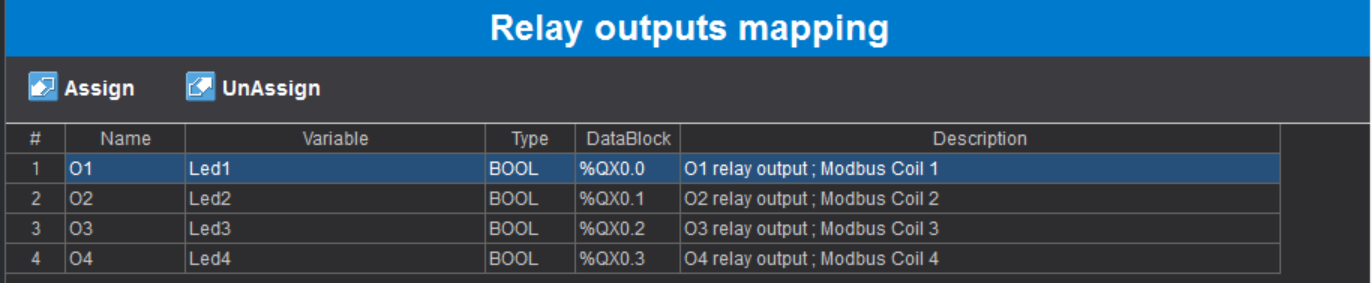
\includegraphics[width=0.9\linewidth]{09_relay_outputs_mapping.png}
    \caption{Mapeo de salidas de relé: \texttt{Led1} a \texttt{Led4} en
    \texttt{O1} a \texttt{O4}.}
    \label{fig:plcide_outputs}
\end{figure}

% -------------------------------------------------
\subsubsection{Programación en Ladder Diagram}
\label{subsubsec:p1_ladder}

\paragraph{Red 0001: arranque/paro con autoenclave}
\label{par:negado}
La figura~\ref{fig:ladder_autoenclave} muestra la Red 0001 terminada. Con
doble clic sobre cada símbolo sin asignar de la red recién creada se
asignan los nombres: primer contacto \texttt{Start}, segundo contacto
\texttt{Run}, bobina \texttt{Running}. Así, la red queda
\texttt{--[Start]--[Run]--(\,Running\,)--}, pero \texttt{Running} solo se
energiza mientras \texttt{Start} está presionado y se apaga en cuanto se
suelta: no hay memoria de estado.

\begin{figure}[H]
    \centering
    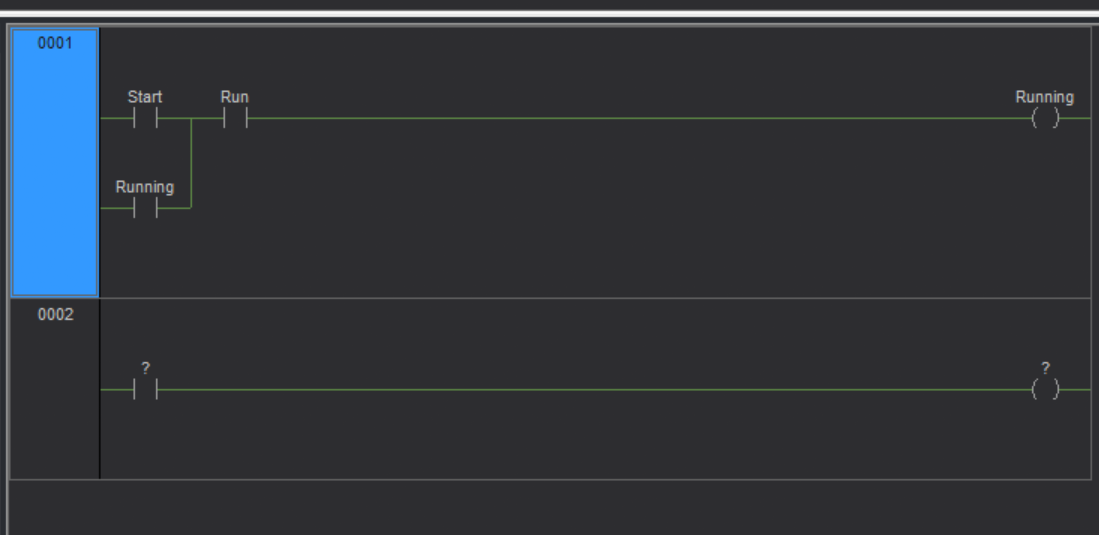
\includegraphics[width=0.9\linewidth]{11_ladder_autoenclave.png}
    \caption{Red 0001 con el autoenclave agregado.}
    \label{fig:ladder_autoenclave}
\end{figure}

La solución es un autoenclave (\emph{seal-in}): un contacto
\texttt{Running} en paralelo con \texttt{Start}, agregado con clic derecho
sobre \texttt{Start} $\to$ \ui{New Parallel contact} (el menú contextual
se muestra en la figura~\ref{fig:ladder_menu}) y nombrado también
\texttt{Running}.

La lógica resultante es (Start O Running) Y Run $\to$ Running:
\texttt{Start} es el pulso momentáneo que \emph{inicia} la secuencia;
\texttt{Running} en paralelo es el autoenclave, que usa el propio bit de la
bobina para sostenerse una vez que \texttt{Start} ya se soltó; y
\texttt{Run} es la condición de permiso continuo: como está en serie con todo lo
demás, basta con que se abra (se presione el pulsador~2) para cortar la
salida sin importar el estado de \texttt{Start}/\texttt{Running}. Es el
patrón clásico de ``arranque-paro con enclave'', el mismo que se arma con
relés físicos, aquí con bits internos del PLC.

Falta un detalle sobre \texttt{Run}. Como el pulsador~2 entrega 1 solo
mientras se presiona y 0 en reposo, pero la lógica necesita que el permiso
de marcha esté en 1 en reposo, se niega el contacto: clic derecho sobre
\texttt{Run} en la Red 0001 $\to$ \ui{Negate contact} (símbolo
\texttt{/}). El contacto negado se ve en la Red 0001 de la
figura~\ref{fig:ladder_negado}, más adelante. Con esto, mientras el
pulsador esté sin presionar el contacto negado lee 1 (permiso activo); al
presionarlo, el contacto negado lee 0 y corta \texttt{Running}, parando
todo en cascada.

\begin{nota}
Si en una instalación particular el pulsador~2 está cableado como contacto
NC real (entrega 1 en reposo y 0 al presionar), el contacto \texttt{Run}
debe dejarse normal (no negado); lo importante es que la variable
interna refleje siempre ``1~=~permiso de marcha''.
\end{nota}

\paragraph{Redes 0002 y 0003: Led1 inmediato y Timer1}
La Red 0002 es la primera etapa de la secuencia:
\texttt{--[Running]--(\,Led1\,)--}. En cuanto se presiona el pulsador~1,
la Red 0001 pone \texttt{Running} en 1 y lo sostiene con el autoenclave;
en ese mismo ciclo de escaneo el contacto \texttt{Running} de la Red 0002
se cierra y energiza \texttt{Led1}, que avanza el cilindro~1 en FluidSIM.
\texttt{Led1} permanece encendido mientras \texttt{Running} siga en 1, y
se apaga en cuanto el pulsador~2 corta el permiso de marcha.

La Red 0003 debe medir el tiempo que transcurre desde el arranque, así que
necesita un temporizador: el bloque de función \texttt{TON}
(temporizador a la conexión). Para insertarlo se da clic derecho sobre el
elemento de la izquierda de la red (el contacto \texttt{Running}), con lo
que se despliega el menú contextual de la figura~\ref{fig:ladder_menu};
ahí se elige \ui{New Block}, se busca el tipo \texttt{TON} y se nombra la
instancia \texttt{Timer1}.

\begin{figure}[H]
    \centering
    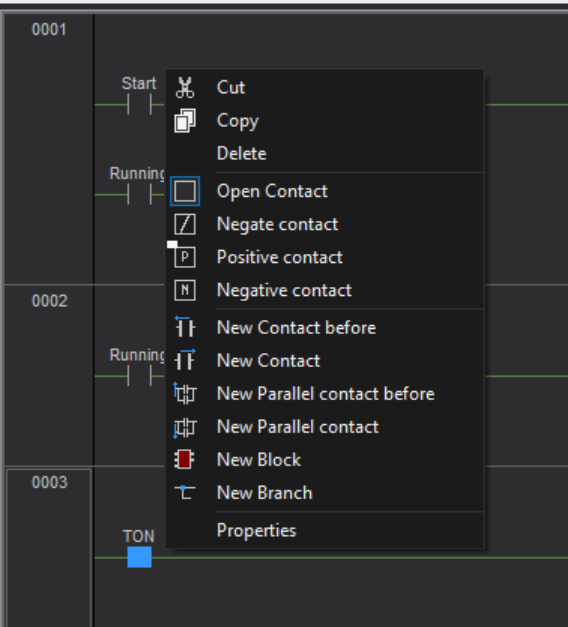
\includegraphics[width=0.7\linewidth]{12_menu_contextual_contacto.png}
    \caption{Menú contextual para insertar elementos sobre un contacto.}
    \label{fig:ladder_menu}
\end{figure}

La figura~\ref{fig:ladder_negado} muestra el resultado: las Redes 0001 a
0003 con el contacto \texttt{Run} ya negado y el bloque \texttt{Timer1}
en la Red 0003.

\begin{figure}[!t]
    \centering
    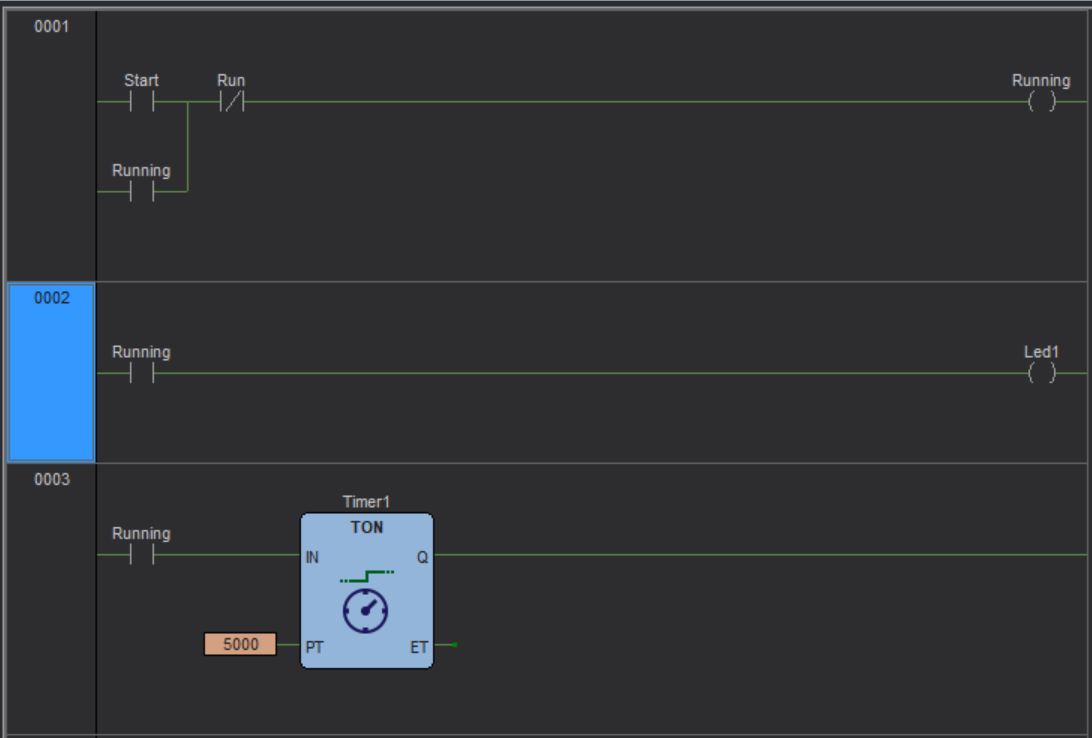
\includegraphics[width=0.9\linewidth]{16_run_negado.png}
    \caption{Contacto \texttt{Run} negado.}
    \label{fig:ladder_negado}
\end{figure}

El bloque \texttt{TON} tiene cuatro pines:
\begin{itemize}
    \item \texttt{IN}: la condición que arranca el conteo. Se conecta al
    contacto \texttt{Running}, así que \texttt{Timer1} empieza a contar en
    el mismo instante en que se enciende \texttt{Led1}.
    \item \texttt{PT} (\emph{preset time}): el tiempo que debe transcurrir
    antes de activar la salida. Se escribe con doble clic sobre el pin, en
    milisegundos. La autora usó 5~s (\texttt{5000}), pero el valor puede
    variarse libremente según el ritmo que se quiera para la secuencia.
    \item \texttt{Q}: la salida, que pasa a 1 cuando el tiempo transcurrido
    alcanza \texttt{PT} y se mantiene así mientras \texttt{IN} siga en 1.
    \item \texttt{ET} (\emph{elapsed time}): el tiempo transcurrido desde
    que \texttt{IN} pasó a 1; vuelve a cero cuando \texttt{IN} cae a 0.
\end{itemize}

\paragraph{Red 0004: Led2 al terminar Timer1}
Cuando \texttt{Timer1} completa sus 5~s, su salida \texttt{Q} pasa a 1. La
Red 0004 usa justamente esa salida como contacto,
\texttt{--[Timer1.Q]--(\,Led2\,)--}, para encender \texttt{Led2}: es el
paso al segundo estado de la secuencia. \texttt{Led1} sigue encendido,
porque \texttt{Running} no ha cambiado.

\begin{figure}[H]
    \centering
    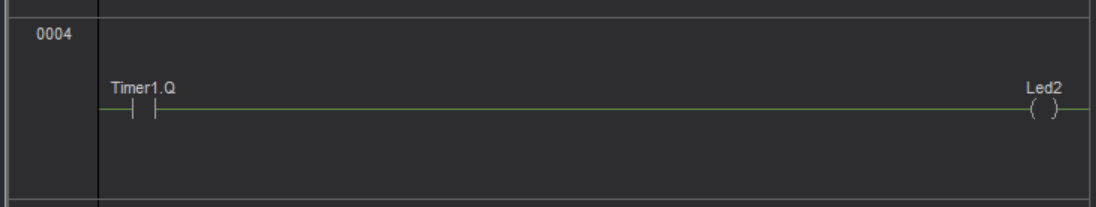
\includegraphics[width=0.9\linewidth]{Red 0004}
    \caption{Red 0004: \texttt{Timer1.Q} enciende \texttt{Led2}.}
    \label{fig:red0004}
\end{figure}

\paragraph{Red 0005: Timer2 para el siguiente estado}
Para pasar al tercer estado hace falta medir otros 5~s, contados desde que
se encendió \texttt{Led2}. Por eso la Red 0005 agrega un segundo bloque
\texttt{TON}, \texttt{Timer2}, insertado igual que \texttt{Timer1}, con el
contacto \texttt{Led2} en su pin \texttt{IN} y \texttt{5000} en
\texttt{PT}: mientras \texttt{Led2} esté encendido, \texttt{Timer2} cuenta.

\begin{figure}[H]
    \centering
    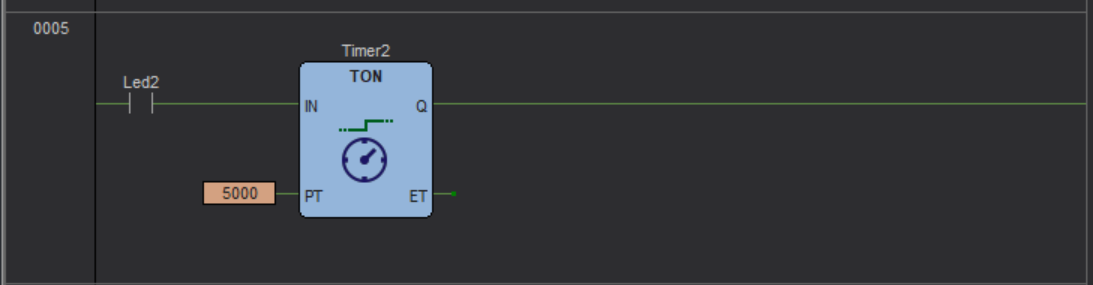
\includegraphics[width=0.9\linewidth]{Red 0005}
    \caption{Red 0005: \texttt{Led2} arranca \texttt{Timer2}.}
    \label{fig:red0005}
\end{figure}

\paragraph{Redes 0006 a 0008: el mismo patrón}
A estas alturas ya se nota el patrón: cada estado se compone de una red que
enciende un LED con la salida \texttt{Q} del temporizador anterior y otra
que usa ese LED para arrancar el siguiente temporizador. Las tres redes
restantes lo repiten (figura~\ref{fig:red0006_0008}): en la Red 0006,
\texttt{Timer2.Q} enciende \texttt{Led3} (10~s desde el arranque); en la
Red 0007, \texttt{Led3} arranca \texttt{Timer3} con otros 5~s; y en la Red
0008, \texttt{Timer3.Q} enciende \texttt{Led4} (15~s desde el arranque).
Al presionar el pulsador~2, \texttt{Running} cae a 0 y la cadena se
deshace en cascada: se apaga \texttt{Led1}, \texttt{Timer1} se reinicia y
apaga \texttt{Led2}, y así sucesivamente hasta \texttt{Led4}.

\begin{figure}[H]
    \centering
    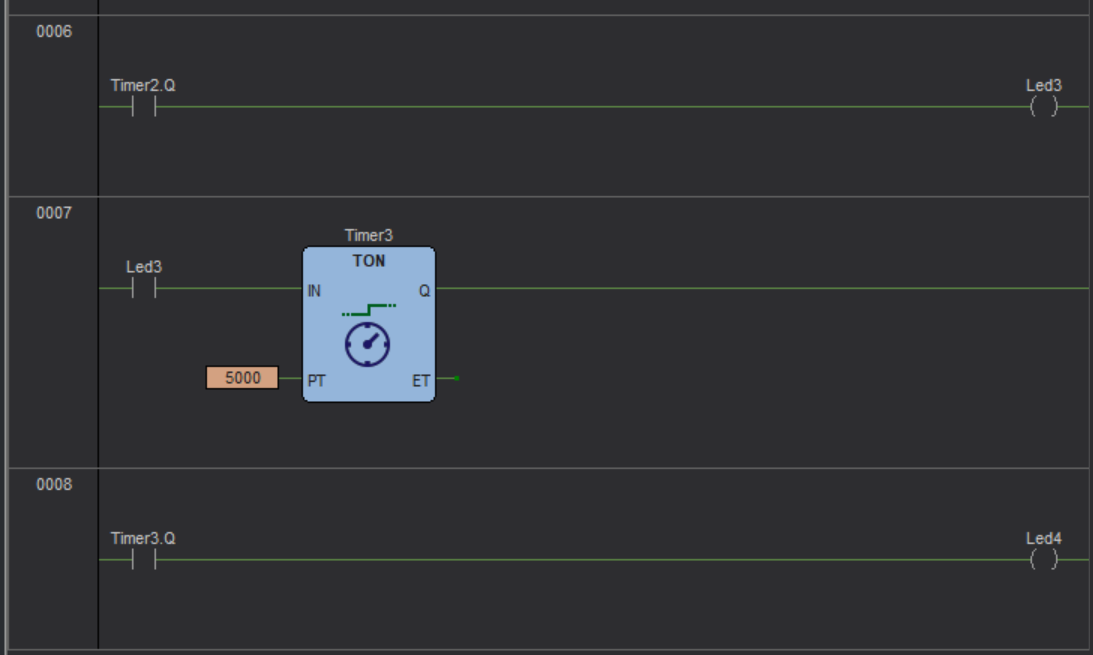
\includegraphics[width=0.9\linewidth]{Red 0006-0007-0008}
    \caption{Redes 0006 a 0008: \texttt{Led3}, \texttt{Timer3} y \texttt{Led4}.}
    \label{fig:red0006_0008}
\end{figure}

La tabla~\ref{tab:cascada} resume las ocho redes del programa completo.

\begin{table}[H]
\centering
\caption{Las ocho redes del programa \texttt{Ejercicio1\_\allowbreak Señales\_\allowbreak Digitales}. Fuente: Autora.}
\label{tab:cascada}
\renewcommand{\arraystretch}{1.4}
\begin{tabularx}{\linewidth}{l X l}
\toprule
\textbf{Red} & \textbf{Lógica} & \textbf{Efecto} \\
\midrule
0001 & (Start O Running) Y /Run $\to$ Running & Arranque/paro con autoenclave \\
0002 & Running $\to$ Led1 & \texttt{Led1} inmediato \\
0003 & Running $\to$ TON \texttt{Timer1} (PT = 5000) & Cuenta 5~s desde el arranque \\
0004 & \texttt{Timer1.Q} $\to$ Led2 & \texttt{Led2} se enciende \\
0005 & Led2 $\to$ TON \texttt{Timer2} (PT = 5000) & Cuenta otros 5~s \\
0006 & \texttt{Timer2.Q} $\to$ Led3 & \texttt{Led3} se enciende \\
0007 & Led3 $\to$ TON \texttt{Timer3} (PT = 5000) & Cuenta otros 5~s \\
0008 & \texttt{Timer3.Q} $\to$ Led4 & \texttt{Led4} se enciende \\
\bottomrule
\end{tabularx}
\end{table}

\begin{nota}
Antes de compilar y descargar el programa, verificar que la expansión
analógica esté identificada en el proyecto, en \ui{I/O Expansions}. El PLC
IDE detecta la expansión conectada al Opta, y si lo declarado en el
proyecto no coincide con lo detectado, la descarga da errores. Para que
aparezca basta con hacer clic en \ui{Scan}; debe quedar como en la
figura~\ref{fig:expansion_analogica}.
\end{nota}

\begin{figure}[H]
    \centering
    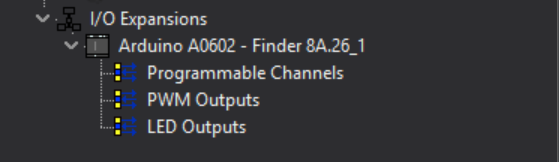
\includegraphics[width=0.55\linewidth]{Expansionanalogica.png}
    \caption{Expansión analógica identificada en \ui{I/O Expansions}.}
    \label{fig:expansion_analogica}
\end{figure}

% -------------------------------------------------
\subsubsection{Montaje en FluidSIM}
\label{subsubsec:p1_fluidsim}

Con el programa ya corriendo en el Opta, se arma la planta virtual que
gobierna. Al abrir FluidSIM aparece un diálogo para elegir las tecnologías
a usar; para este ejercicio se dejan marcadas las tres (Neumática,
Hidráulica y Electrotécnica) y se hace clic en \ui{Iniciar}
(figura~\ref{fig:fs_tecnologias}). El circuito se construye con las tres
capas descritas en la sección~\ref{subsec:intro_fluidsim}.

\begin{figure}[!t]
    \centering
    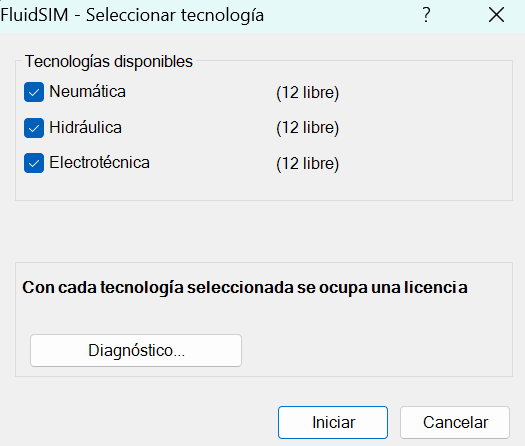
\includegraphics[width=0.6\linewidth]{01_fluidsim_tecnologias.png}
    \caption{Selección de tecnologías al iniciar un proyecto en FluidSIM.}
    \label{fig:fs_tecnologias}
\end{figure}

\paragraph{Actuador: cilindro más válvula 3/2}
Cada uno de los cuatro estados mueve un cilindro, y los cuatro usan el mismo
bloque funcional (figura~\ref{fig:fs_cilindro}): un cilindro de simple
efecto (solo avanza mientras recibe aire; un resorte interno lo retrae
al cortarlo) y una electroválvula 3/2 que controla ese aire. El
accionamiento izquierdo de la válvula es electroneumático: un solenoide
(E1 en el primer cilindro) que la conmuta cuando recibe 24~V. En el
accionamiento derecho se marca la casilla \ui{Con reposición por muelle},
para que la válvula regrese sola a su posición de reposo cuando el
solenoide se desactiva.

Para que la válvula pueda presurizar y despresurizar el cilindro, sus vías
se conectan así: la vía~1 a una fuente de aire comprimido, la vía~3 a un
escape y la vía~2 al cilindro. Con el solenoide activado, la válvula une
1 con 2 y el aire comprimido entra al cilindro, que avanza. En reposo, el
muelle la devuelve a la posición que une 2 con 3: el aire del cilindro se
libera por el escape y el resorte interno lo retrae. Sin el escape, el
aire quedaría atrapado en el cilindro y este no podría volver.

\begin{figure}[H]
    \centering
    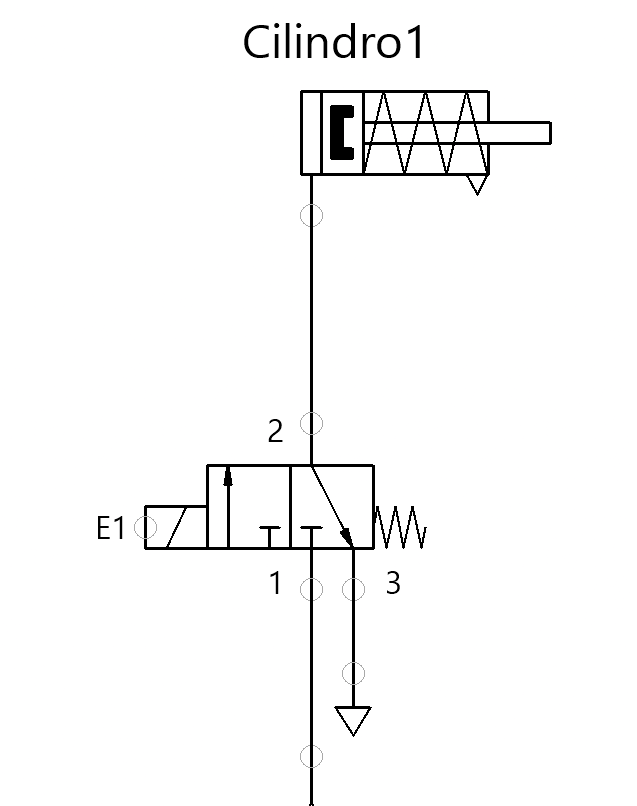
\includegraphics[width=0.3\linewidth]{02_cilindro_valvula.png}
    \caption{Cilindro de simple efecto con válvula 3/2 con reposición por muelle.}
    \label{fig:fs_cilindro}
\end{figure}

\paragraph{Montaje de reacción para un estado}
Antes de armar el circuito completo conviene entender el montaje de un solo
estado (figura~\ref{fig:fs_minimo}); el circuito completo no es más que
este mismo montaje repetido una vez por cada estado.

\begin{figure}[!htb]
    \centering
    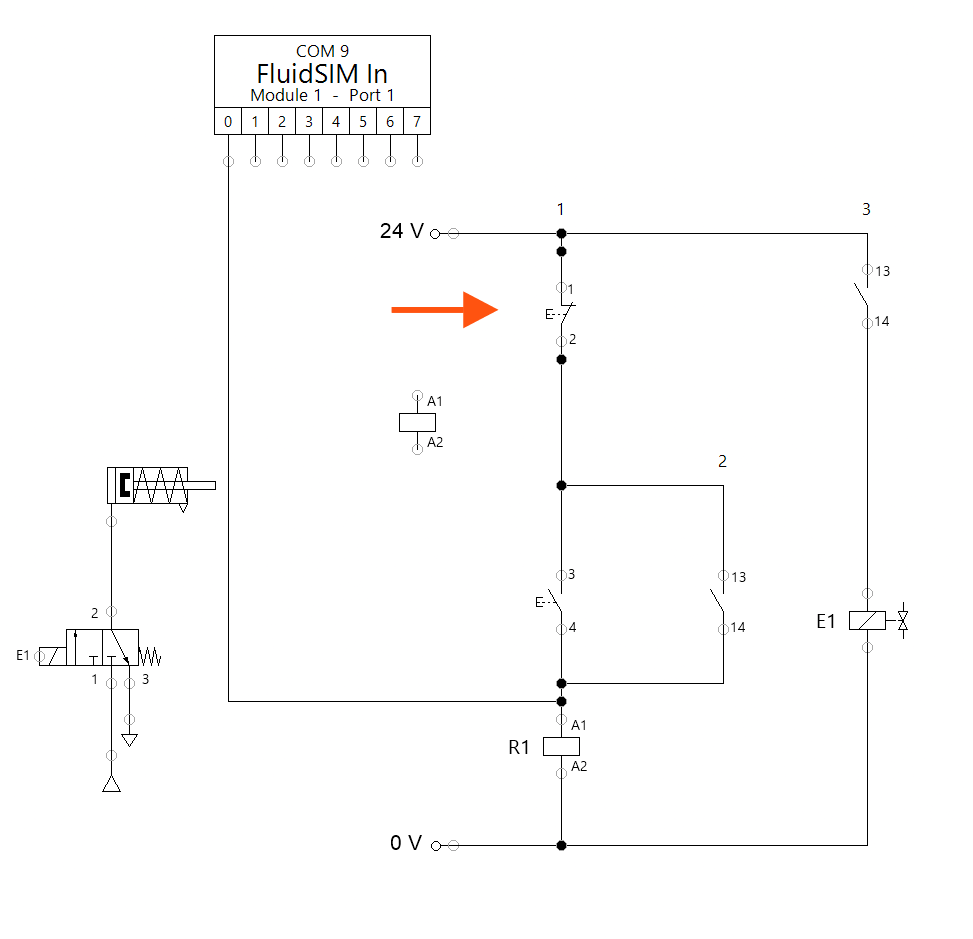
\includegraphics[width=0.75\linewidth]{05_circuito_cilindro1_simple.png}
    \caption{Montaje de reacción para un estado: entrada del EasyPort, relé
    R1 con autoenclave y solenoide E1.}
    \label{fig:fs_minimo}
\end{figure}

El montaje se recorre de la entrada a la potencia:

\begin{enumerate}
    \item Entrada. Se coloca el bloque \ui{FluidSIM In}, que se encuentra
    en la categoría EasyPort de la biblioteca
    (sección~\ref{subsubsec:fs_easyport}). Su canal~0 se conecta a la bobina
    del relé R1: cuando por ese canal llega un 1 lógico, R1 se energiza.
    \item Autoenclave. Al energizarse, R1 cierra su contacto 13--14, que
    está en paralelo con el pulsador (contacto obturador, NA). Ese contacto
    sigue alimentando la bobina de R1 aunque la señal de entrada
    desaparezca, de modo que el estado se mantiene activo: es el mismo
    autoenclave de la Red 0001 del programa Ladder, ahora hecho con un relé.
    El pulsador también puede accionarse a mano, haciendo clic sobre él
    mientras la simulación está en curso; pero, como es un pulsador sin
    enclavamiento, se desactiva en cuanto se suelta, y si R1 no llegó a
    enclavarse el estado se pierde.
    \item Paro. En serie con el conjunto anterior hay un contacto
    franqueador (NC), señalado con la flecha naranja en la figura. Al
    accionarse abre la rama, corta la energía de la bobina de R1 y apaga el
    estado. Más adelante, este franqueador se accionará de forma externa
    con el pulsador~2 (\texttt{Run}), del mismo modo que la activación de
    R1 con 24~V se accionará con el pulsador~1 (\texttt{Start}).
    \item Potencia. En la rama de la derecha, un segundo contacto de R1
    está en serie con el solenoide de válvula E1. E1 es el accionamiento
    izquierdo de la electroválvula de la figura~\ref{fig:fs_cilindro}:
    mientras R1 está energizado, E1 conmuta la válvula y el cilindro
    avanza; cuando R1 cae, el muelle devuelve la válvula y el cilindro se
    retrae.
\end{enumerate}

\paragraph{Circuito completo del ejercicio}
El circuito completo (figura~\ref{fig:fs_completo}) repite el montaje de
reacción cuatro veces, una por estado: relés R1 a R4, solenoides E1 a E4 y
\texttt{Cilindro1} a \texttt{Cilindro4}, cada uno con su electroválvula
3/2 a la izquierda del esquema. Las cuatro etapas comparten la misma línea
de 24~V y 0~V y los mismos dos bloques del EasyPort, \ui{FluidSIM In} y
\ui{FluidSIM Out}. El mismo circuito se reproduce a página completa en
el~\ref{app:circuito}; como la figura es vectorial, se puede ampliar sin
perder nitidez.

La parada incondicional se resuelve con el relé S1, a la izquierda del
esquema: el canal~0 del bloque \ui{FluidSIM In} se deja conectado a la
bobina de S1, de modo que S1 es el que se acciona cuando se presiona el
pulsador de parada. Para que S1 corte las cuatro etapas a la vez, todos los
franqueadores del circuito deben estar relacionados con S1. Con doble clic
sobre cada franqueador se abre su ventana \ui{Contacto}
(figura~\ref{fig:rele_s1}); ahí, en \ui{Objeto relacionado}, se selecciona
\texttt{S1} (el campo \ui{Variable definida previamente} pasa a mostrar
\texttt{S1.state}) y se hace clic en \ui{Aceptar}. Así, al energizarse
S1, los cuatro franqueadores se abren al mismo tiempo y todos los relés
R1 a R4 se desenclavan.

\begin{figure}[H]
    \centering
    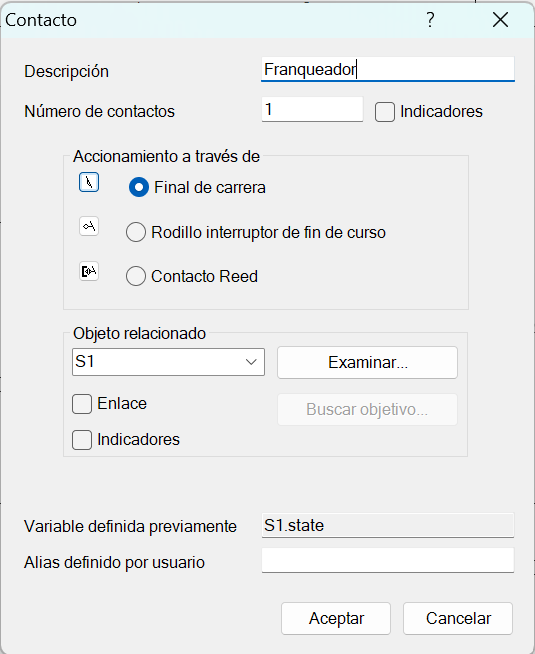
\includegraphics[width=0.45\linewidth]{rele_S1.png}
    \caption{Ventana \ui{Contacto} de un franqueador, relacionado con el
    relé \texttt{S1}.}
    \label{fig:rele_s1}
\end{figure}

\begin{figure}[H]
    \centering
    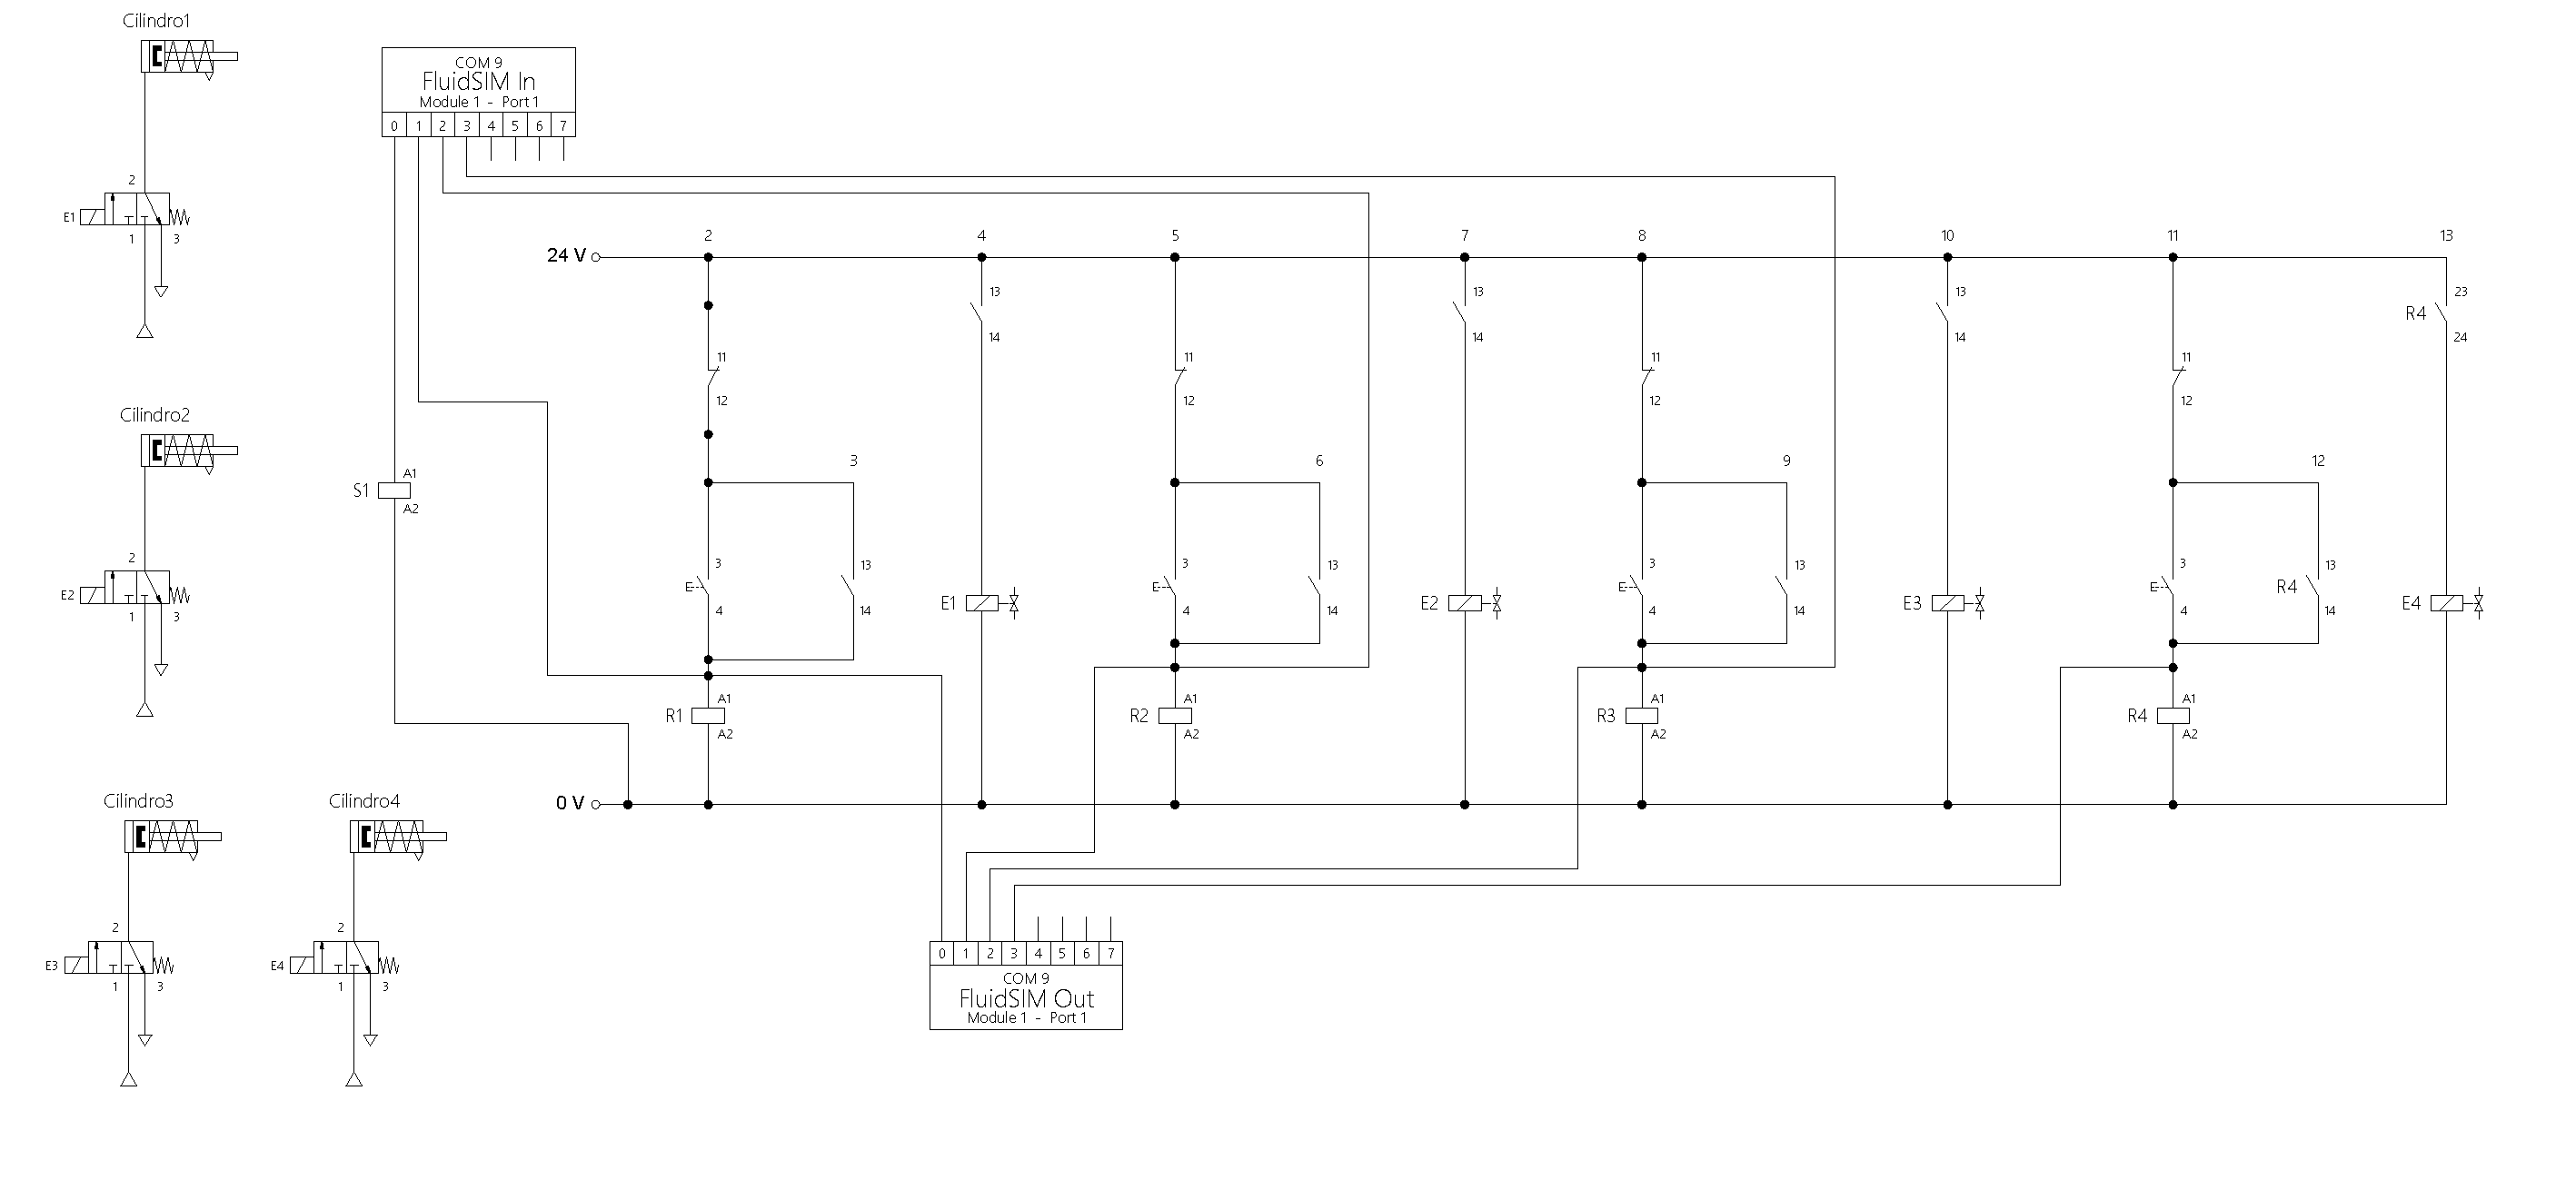
\includegraphics[width=\linewidth, trim=20 45 45 3, clip]{Ejercicio1_completo.pdf}
    \caption{Circuito completo del ejercicio: cuatro etapas con relés R1 a
    R4, solenoides E1 a E4 y sus cilindros.}
    \label{fig:fs_completo}
\end{figure}

\paragraph{Enlace con el Opta}
Los dos bloques del circuito usan el mismo EasyPort: \texttt{Module~1},
\texttt{Port~1}, y el puerto COM que Windows le asigne al EasyPort en cada
computador (en la figura, \texttt{COM~9}). Para cablearlo y ponerlo en
marcha se sigue el orden de la sección~\ref{subsubsec:puesta_marcha}, con
los colores de hilo de la tabla~\ref{tab:syslink}.

Las señales recorren tres tramos (tabla~\ref{tab:conexiones_p1}):

\begin{enumerate}
    \item Pulsadores $\to$ Opta. Los dos pulsadores van a la bornera
    \textsc{digital input} de la plataforma: el pulsador~1 (\texttt{Start})
    al hilo verde~1 y el pulsador~2 (\texttt{Run}) al hilo verde~2. El
    Opta los lee directamente en sus entradas \texttt{I1} e \texttt{I2}.
    \item Opta $\to$ EasyPort. Las salidas de relé que se programaron en
    Ladder (\texttt{Led1} a \texttt{Led4}) salen por la bornera
    \textsc{relay output}, en los hilos café etiquetados 1 a 4, y van a
    las entradas 0 a 3 del EasyPort. En FluidSIM esas señales llegan por los
    canales 0 a 3 del bloque \ui{FluidSIM In}.
    \item EasyPort $\to$ LEDs. Los canales 0 a 3 del bloque
    \ui{FluidSIM Out} salen por las salidas 0 a 3 del EasyPort, que van a
    las borneras \textsc{easyport output}; ahí se conecta, respectivamente,
    cada una de las cuatro luces LED de 24~V.
\end{enumerate}

\begin{table}[H]
\centering
\caption{Conexiones de la Práctica~1. Los colores del cable SysLink son los
de la tabla~\ref{tab:syslink}. Fuente: Autora.}
\label{tab:conexiones_p1}
\linespread{1}\small\selectfont
\renewcommand{\arraystretch}{1.2}
\begin{tabularx}{\linewidth}{l X X}
\toprule
\textbf{Señal} & \textbf{Desde} & \textbf{Hacia} \\
\midrule
\multicolumn{3}{l}{\textit{Pulsadores $\rightarrow$ entradas del Opta}} \\
\midrule
\texttt{Start} & Pulsador~1 & \textsc{digital input}, \hilo{HiloVerde}{HiloVerde}~verde~1 (\texttt{I1}) \\
\texttt{Run}   & Pulsador~2 & \textsc{digital input}, \hilo{HiloVerde}{HiloVerde}~verde~2 (\texttt{I2}) \\
\midrule
\multicolumn{3}{l}{\textit{Salidas de relé del Opta $\rightarrow$ entradas del EasyPort (\ui{FluidSIM In})}} \\
\midrule
\texttt{Led1} & \textsc{relay output}, \hilo{HiloMarron}{HiloMarron}~café~1 & Entrada~0, pin~13, \hilo{HiloGris}{HiloRosa}~gris/rosa \\
\texttt{Led2} & \textsc{relay output}, \hilo{HiloMarron}{HiloMarron}~café~2 & Entrada~1, pin~14, \hilo{HiloRojo}{HiloAzul}~rojo/azul \\
\texttt{Led3} & \textsc{relay output}, \hilo{HiloMarron}{HiloMarron}~café~3 & Entrada~2, pin~15, \hilo{HiloBlanco}{HiloVerde}~blanco/verde \\
\texttt{Led4} & \textsc{relay output}, \hilo{HiloMarron}{HiloMarron}~café~4 & Entrada~3, pin~16, \hilo{HiloMarron}{HiloVerde}~marrón/verde \\
\midrule
\multicolumn{3}{l}{\textit{Salidas del EasyPort (\ui{FluidSIM Out}) $\rightarrow$ luces LED}} \\
\midrule
Canal 0 & Salida~0, pin~1, \hilo{HiloBlanco}{HiloBlanco}~blanco & \textsc{easyport output}~0 $\rightarrow$ LED~1 \\
Canal 1 & Salida~1, pin~2, \hilo{HiloMarron}{HiloMarron}~marrón & \textsc{easyport output}~1 $\rightarrow$ LED~2 \\
Canal 2 & Salida~2, pin~3, \hilo{HiloVerde}{HiloVerde}~verde & \textsc{easyport output}~2 $\rightarrow$ LED~3 \\
Canal 3 & Salida~3, pin~4, \hilo{HiloAmarillo}{HiloAmarillo}~amarillo & \textsc{easyport output}~3 $\rightarrow$ LED~4 \\
\bottomrule
\end{tabularx}
\end{table}

La figura~\ref{fig:diagrama_p1} reúne los tres tramos en un solo diagrama
eléctrico: la alimentación de 24~V desde el SIMUL8, los pulsadores en las
entradas del Opta, las salidas de relé hacia las entradas del EasyPort y
las luces LED en sus salidas.

\begin{figure}[H]
    \centering
    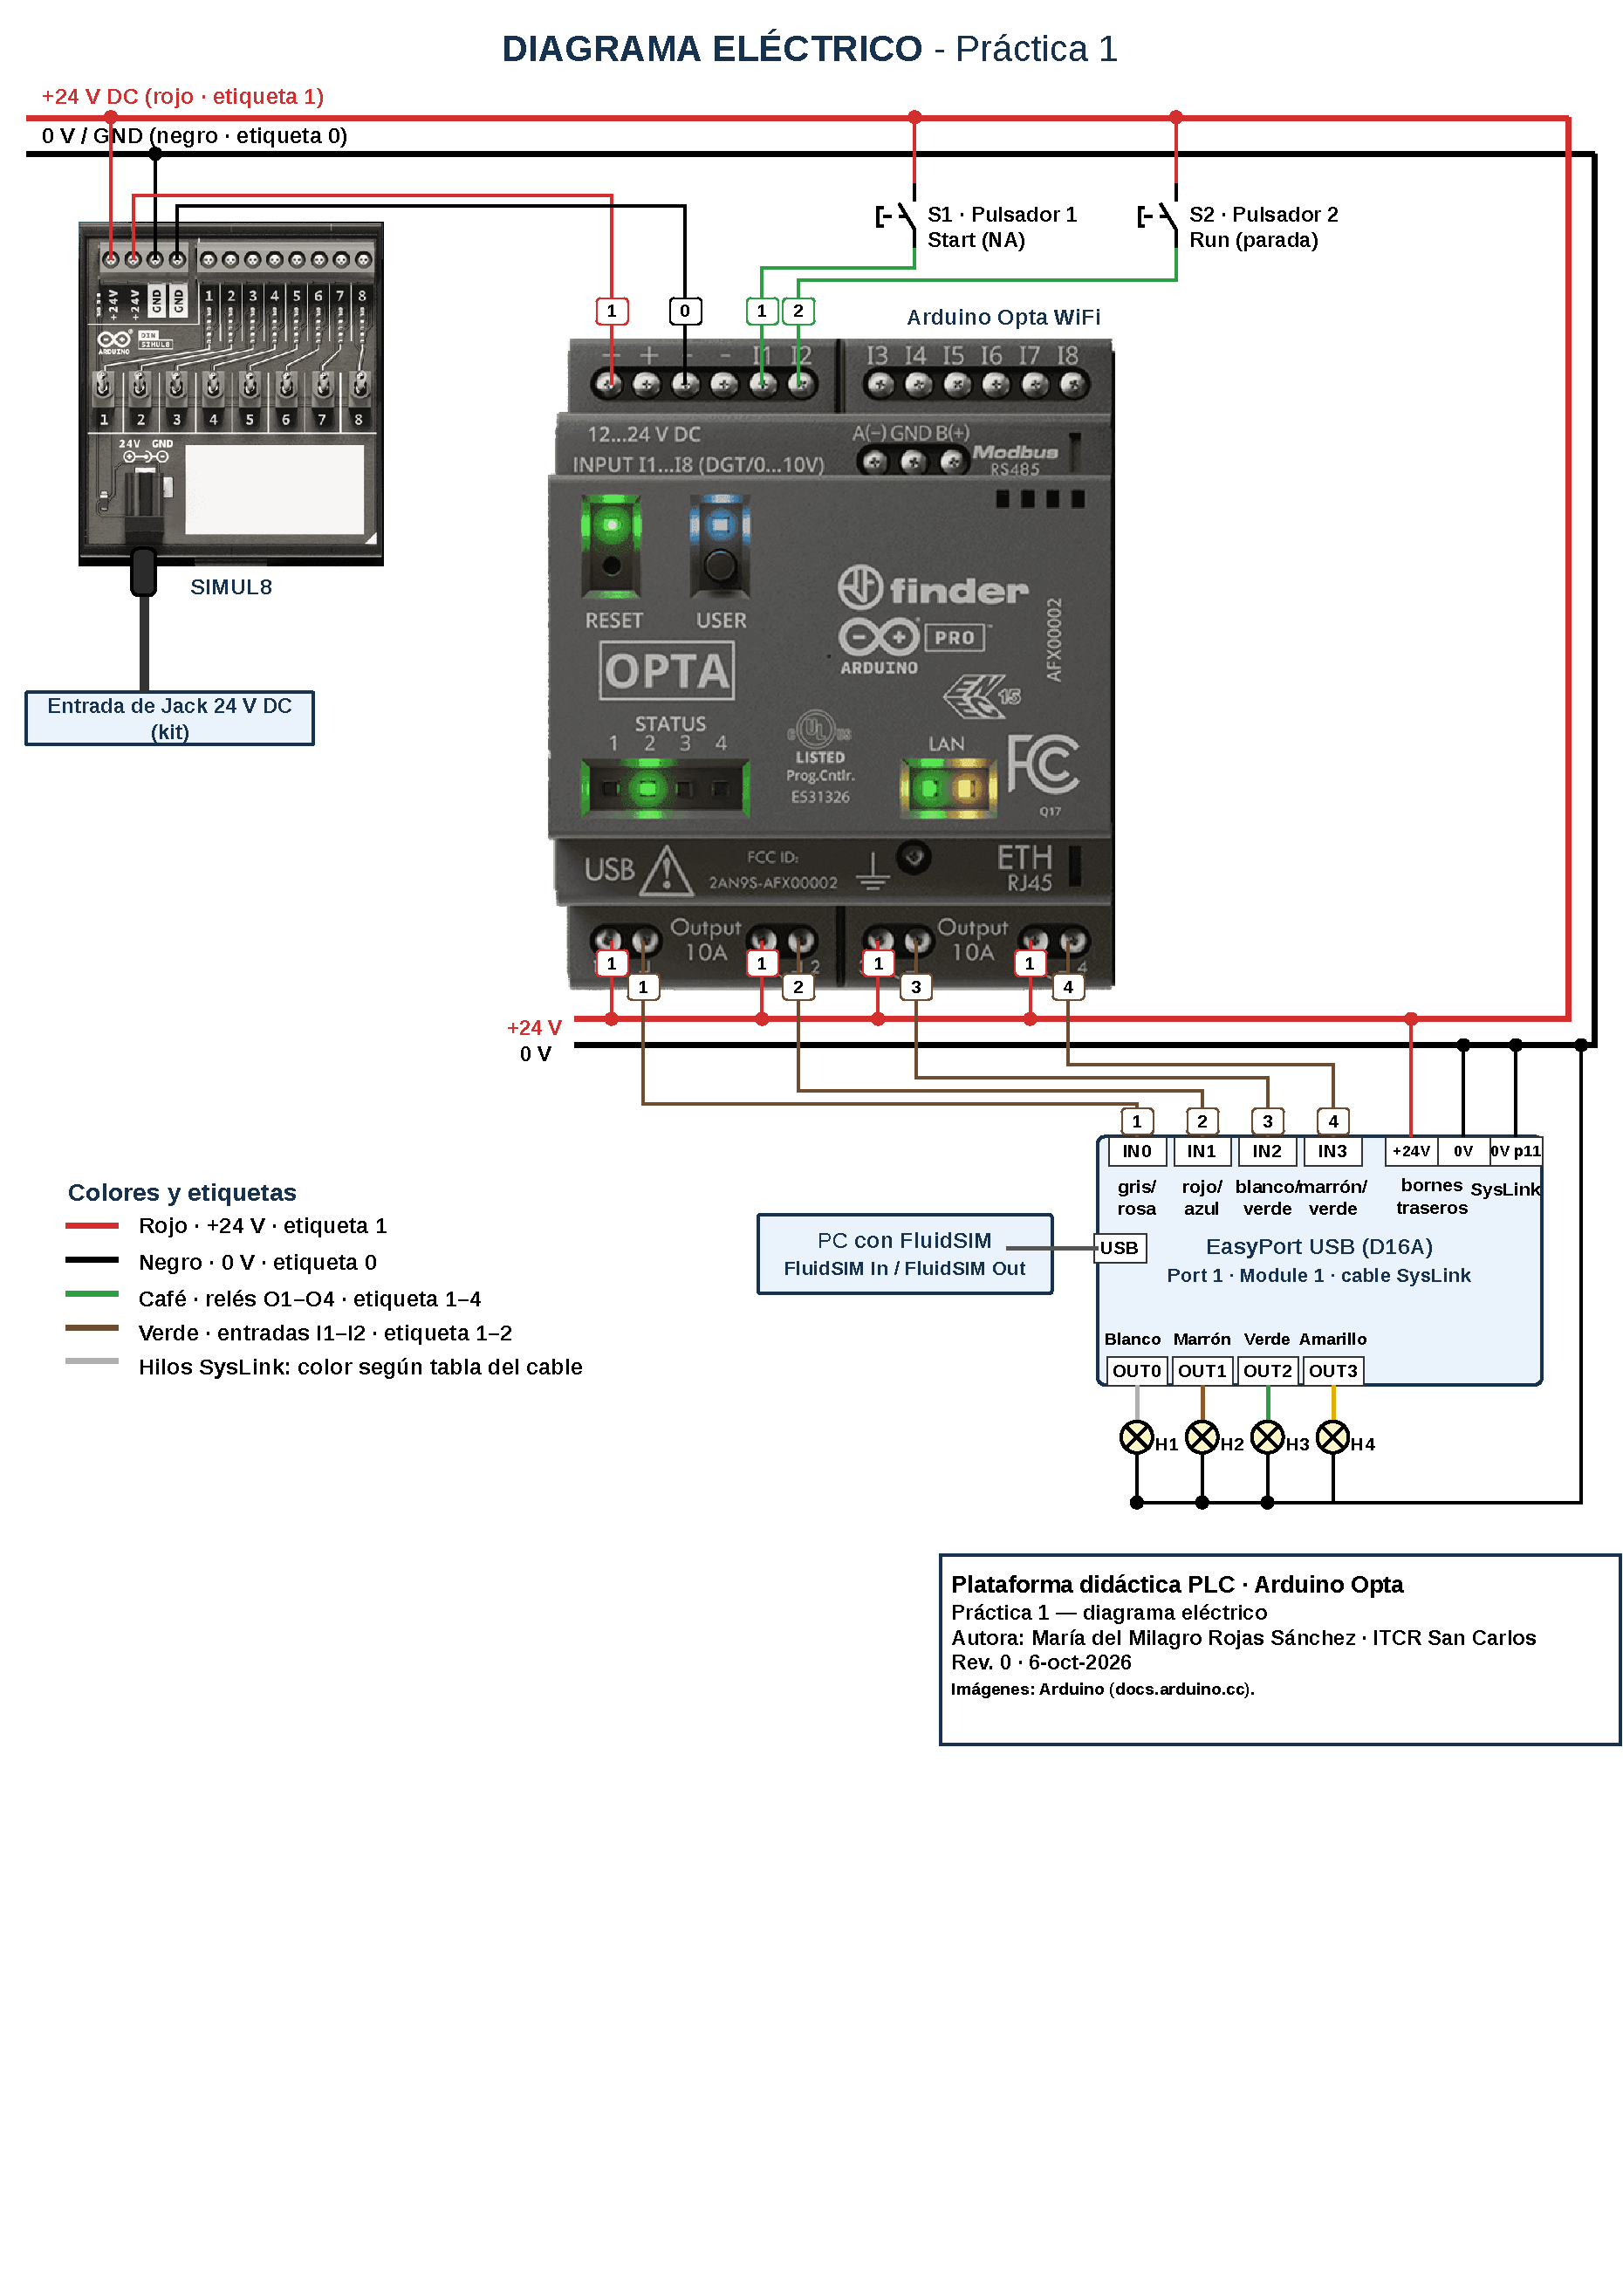
\includegraphics[width=\linewidth,trim=6 290 0 8,clip]{Diagrama_Electrico_Practica1.pdf}
    \caption{Diagrama eléctrico de las conexiones usadas en la
    Práctica~1. Fuente: Autora.}
    \label{fig:diagrama_p1}
\end{figure}

% -------------------------------------------------
% Práctica 2 (parte Ladder). Fuente: practica2_ladder_para_code/
% (borrador de la autora + ESPECIFICACION_TECNICA.md). Sin parte FluidSIM:
% la señal analógica se visualiza en la pantalla del EasyPort.
% -------------------------------------------------
\subsection[Práctica 2: sistema de enfriamiento con ventilación regulable]{Práctica 2: sistema de enfriamiento con ventilación regulable, con DIN Celsius, expansión analógica y PWM}
\label{subsec:practica2}

\begin{practica}{Sistema de enfriamiento con ventilación regulable}
\textbf{Objetivo.} Simular un caso industrial frecuente: un recinto que
se calienta (una sala de equipos, un tablero eléctrico, una cámara de
proceso) y un ventilador cuya velocidad se ajusta según la temperatura. La
placa DIN Celsius representa el recinto: su sensor mide la temperatura y
sus dos calentadores, que se encienden y apagan con pulsadores, representan
las cargas que aportan calor. El Opta lee la temperatura con la expansión
de señales analógicas, la convierte a grados Celsius y la compara con la
temperatura deseada; la salida del controlador, programado en Ladder, se
entrega por dos vías: una salida PWM que regula la velocidad del motor del
ventilador y una salida analógica de 0 a 10~V que lleva la misma señal al
EasyPort, donde se visualiza en su pantalla.\\
\textbf{Materiales.} Plataforma didáctica de PLC (Arduino Opta WiFi),
expansión Opta Ext A0602 (AFX00007) con firmware 0.1.8 o superior, placa
DIN Celsius, DIN Simul8 (pulsadores), motor de corriente continua de 24~V
y 0,5~A como ventilador, fuente de 24~V del panel, EasyPort D16A,
multímetro, cables, computador con PLC IDE instalado. Arduino
IDE solo si hay que actualizar el firmware de la expansión
(\ref{app:firmware}).\\
\textbf{Montaje.} Físico. El sensor de la DIN Celsius se conecta a la
entrada \texttt{I1} de la expansión; las salidas de relé \texttt{O1} y
\texttt{O2} del Opta alimentan los dos calentadores de la placa; el motor
se conecta entre la salida \texttt{P1} de la expansión y tierra, y la
alimentación \texttt{VPWM} de la expansión viene de los 24~V del panel.
La salida analógica \texttt{O1} de la expansión se lleva al pin~8 (cable
amarillo) del conector analógico del EasyPort, y su negativo a la tierra
común; esa señal se lee en el canal~0 de las entradas de la pantalla del
EasyPort. Los bornes de cada conexión están en la
figura~\ref{fig:diagrama_p2}.\\
\textbf{Flujo.} Primero se verifica la expansión y su firmware
(sección~\ref{subsubsec:p2_hw}); después se crea el programa, se mapean
las entradas y salidas y se escriben las dieciséis redes
(secciones~\ref{subsubsec:p2_programa} a~\ref{subsubsec:p2_ladder}); por
último se descarga y se verifica en línea
(sección~\ref{subsubsec:p2_verif}); al final se comprueba la señal
analógica en la pantalla del EasyPort
(sección~\ref{subsubsec:p2_pantalla}). Esta práctica no usa FluidSIM.
\end{practica}

\subsubsection{Descripción del ejercicio}
\label{subsubsec:p2_desc}

En la industria, muchos recintos deben mantenerse por debajo de una
temperatura máxima: salas de servidores, tableros eléctricos con
variadores y fuentes, cámaras de secado o de proceso. Un ventilador a
velocidad fija desperdicia energía y ruido cuando el calor es poco, y se
queda corto cuando es mucho; por eso se usa ventilación regulable, en la
que un controlador mide la temperatura y ajusta la velocidad del
ventilador a la necesidad del momento. La velocidad se ordena con una
señal PWM, cuando el controlador alimenta directamente un motor de
corriente continua, o con una señal analógica de 0 a 10~V, que es la
referencia de velocidad habitual de un variador de frecuencia.

En esta práctica se arma ese sistema a escala de laboratorio. La placa DIN
Celsius funciona como el recinto que se quiere refrigerar: tiene dos
circuitos calentadores independientes de unos 120~mW cada uno, alimentados
a 24~V, y un sensor de temperatura TMP236 en el centro de la
placa~\cite{celsius}. Los calentadores (las parrillas) hacen el papel de
las cargas que generan calor dentro del recinto, y el operador las
enciende y apaga con pulsadores para provocar los cambios de temperatura.
El motor de corriente continua hace de ventilador. Esta práctica agrega a
lo visto en la Práctica~1 cuatro elementos nuevos: una entrada analógica,
una salida PWM, una salida analógica y aritmética con números reales.

El sistema se comporta así:

\begin{enumerate}
    \item \textbf{Pulsador 1 (\texttt{BOTON1}):} cada pulsación alterna la
    parrilla~1 (calentador izquierdo): si estaba apagada la enciende y
    viceversa.
    \item \textbf{Pulsador 2 (\texttt{BOTON2}):} igual, con la parrilla~2
    (calentador derecho).
    \item \textbf{Pulsador 3 (\texttt{BOTON3}):} mientras se mantiene
    presionado, apaga las dos parrillas.
    \item \textbf{Lectura:} el sensor entrega una tensión proporcional a la
    temperatura del recinto; el Opta la lee, la convierte a grados Celsius
    y la guarda en \texttt{TEMP\_C}.
    \item \textbf{Control:} se calcula el error
    \texttt{ERROR}~=~\texttt{TEMP\_C}~$-$~\texttt{SETPOINT} y la salida del
    controlador, \texttt{PID\_OUT}, entre 0~\% y 100~\%. Es la velocidad
    que se pide al ventilador.
    \item \textbf{Ventilador:} \texttt{PID\_OUT} es directamente el ciclo
    útil del PWM de la salida \texttt{P1} de la expansión; el motor gira
    más rápido cuanto más caliente está el recinto respecto a
    \texttt{SETPOINT}.
    \item \textbf{Señal analógica:} la salida analógica \texttt{O1}
    de la expansión entrega la misma orden como una tensión de 0 a 10~V
    (0~V con \texttt{PID\_OUT}~=~0~\%, 10~V con 100~\%), que se conecta al
    EasyPort y se visualiza en su pantalla.
\end{enumerate}

Con \texttt{SETPOINT}~=~28~$^\circ$C y una ganancia \texttt{KP}~=~5, el
motor permanece detenido a 28~$^\circ$C o menos, gira al 50~\% a
38~$^\circ$C y llega al 100~\% a 48~$^\circ$C. La autora eligió estos valores a partir
de las temperaturas que alcanza la placa: con una sola parrilla encendida
y 25~$^\circ$C de ambiente se midieron entre 37 y 38~$^\circ$C, con
31~$^\circ$C de ambiente entre 39 y 40~$^\circ$C, y con las dos parrillas
entre 45 y 47~$^\circ$C.

\begin{nota}
En una instalación real el aire del ventilador baja la temperatura del
recinto y el lazo se cierra: el controlador mide el efecto de su propia
acción. En el banco, el motor representa al ventilador pero no enfría la
placa, de modo que el lazo no es de verdad cerrado. Por eso, de las
acciones de un controlador PID solo se usa la proporcional: con un
actuador que no corrige el error, el acumulador de la integral crecería
sin control. Las redes de la integral (0011 y 0012) se dejan escritas con
\texttt{KI}~=~0 para que no tengan efecto y puedan activarse en una planta
que sí responda.
\end{nota}

% -------------------------------------------------
\subsubsection{Preparación del hardware}
\label{subsubsec:p2_hw}

Antes de abrir el programa se verifican dos cosas de la expansión.

\paragraph{Expansión identificada}
Como en la Práctica~1 (figura~\ref{fig:expansion_analogica}), en
\ui{I/O Expansions} debe aparecer la \ui{Arduino A0602 - Finder 8A.26} y,
tras hacer clic en \ui{Scan}, la columna \ui{Project Config} debe coincidir
con \ui{Detected Config} (figura~\ref{fig:p2_io_verde}).

\begin{figure}[H]
    \centering
    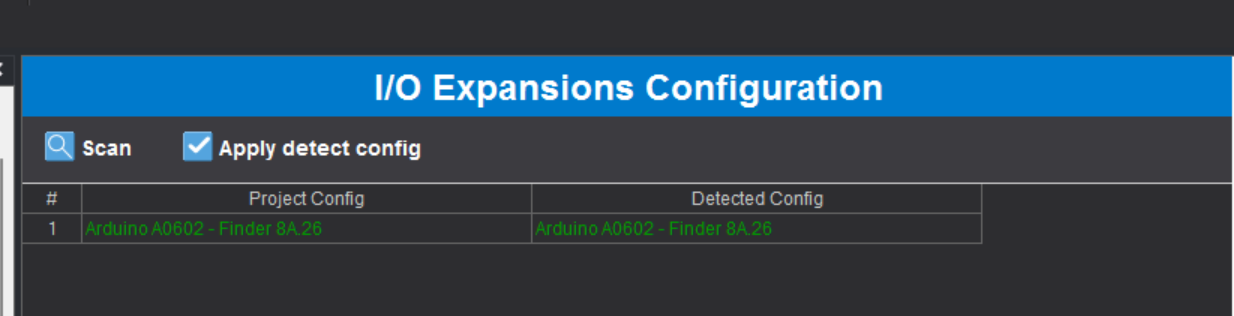
\includegraphics[width=0.75\linewidth]{p2_io_expansions_verde.png}
    \caption{Ventana \ui{I/O Expansions Configuration}: la configuración
    del proyecto coincide con la detectada.}
    \label{fig:p2_io_verde}
\end{figure}

\paragraph{Firmware de la expansión}
Para que el PLC IDE pueda leer y escribir los canales de la expansión, esta
debe tener el firmware 0.1.8 o superior~\cite{optaanalogtut}. La expansión
usada traía la versión 0.1.4; con ella la lectura analógica funcionaba,
pero la salida PWM no respondía a los cambios del ancho de pulso (un LED de
prueba quedaba fijo) aunque el programa mostraba \texttt{PWM\_OK} en
\texttt{TRUE}. Se actualizó a la 0.1.14 siguiendo el procedimiento
del~\ref{app:firmware}, y desde entonces la salida PWM responde.

\begin{advertencia}
Actualizar el firmware con el sketch de Arduino IDE sobrescribe el programa
que corre en el Opta. Al terminar, en el PLC IDE hay que volver a descargar
el \emph{runtime} al Opta y reconectar antes de seguir
(\ref{app:firmware}).
\end{advertencia}

% -------------------------------------------------
\subsubsection{Creación del programa Ladder}
\label{subsubsec:p2_programa}

Se sigue el procedimiento de la sección~\ref{subsubsec:p1_programa}. Datos
de este ejercicio:

\begin{enumerate}
    \item Proyecto: \texttt{Ejercicio2\_\allowbreak Ladder\_\allowbreak analog}.
    \item Programa nuevo de lenguaje \ui{LD} con el nombre
    \texttt{Sistema\_\allowbreak de\_\allowbreak enfriamiento}. Se asigna a
    la tarea \ui{Fast} desde el campo \ui{Assign to} de la ventana
    \ui{New program}, o después desde \menu{Project}{Tasks} $\to$ \ui{Fast}
    (figura~\ref{fig:p2_arbol}).
    \item Con doble clic en \menu{Tasks}{Fast} se abre \ui{Tasks
    configuration}. En la fila \ui{Fast} se pone \ui{Set period} en
    \ui{Yes} y \ui{Period (ms)} en \texttt{50}
    (figura~\ref{fig:p2_tasks}).
\end{enumerate}

\begin{figure}[H]
    \centering
    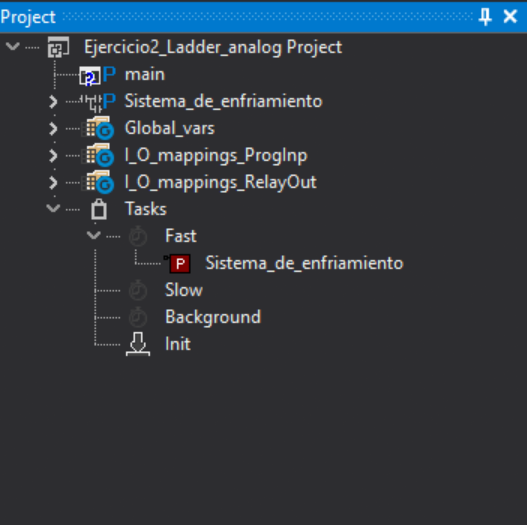
\includegraphics[width=0.45\linewidth]{p2_arbol_tasks.png}
    \caption{Árbol del proyecto con el programa
    \texttt{Sistema\_\allowbreak de\_\allowbreak enfriamiento} asignado a
    la tarea \ui{Fast}.}
    \label{fig:p2_arbol}
\end{figure}

\begin{figure}[H]
    \centering
    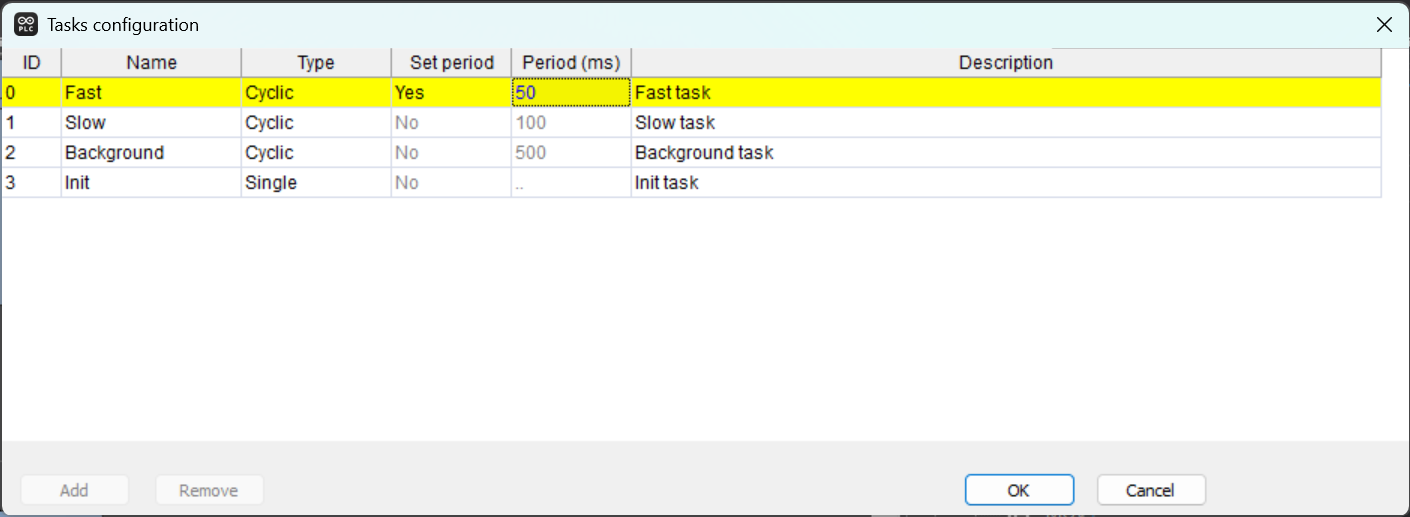
\includegraphics[width=0.85\linewidth]{p2_tasks_50ms.png}
    \caption{Ventana \ui{Tasks configuration} con la tarea \ui{Fast}
    periódica a 50~ms.}
    \label{fig:p2_tasks}
\end{figure}

El periodo de 50~ms es el que Arduino indica para que el \emph{runtime}
pueda cumplir con las acciones programadas sobre la
expansión~\cite{optaanalogtut}. Además fija el valor de la constante
\texttt{KT} (0,05~s) que usa la parte integral del control
(sección~\ref{par:p2_red11}).

\begin{advertencia}
La carpeta del proyecto debe tener un nombre sin tildes ni eñes, en una
ruta corta. La autora creó primero el proyecto como
\texttt{Ejercicio2\_\allowbreak Señales\_\allowbreak Analógicas\_\allowbreak Y\_\allowbreak PWM}
y el compilador falló con errores de memoria
(\texttt{cc1plus.exe: out of memory}) y de argumento inválido
(\emph{Invalid argument}) en una ruta dentro de OneDrive. Con el nombre
\texttt{Ejercicio2\_\allowbreak Ladder\_\allowbreak analog} el proyecto
compiló sin problemas; si los errores vuelven, mover el proyecto a una
carpeta como \texttt{C:\textbackslash PLC\textbackslash}.
\end{advertencia}

% -------------------------------------------------
\subsubsection{Mapeo de entradas y salidas}
\label{subsubsec:p2_mapeo}

Antes de dibujar las redes se da nombre a los canales físicos, como en la
sección~\ref{subsubsec:p1_mapeo}. En esta práctica, además de las entradas
y salidas del Opta, se mapean canales de la expansión A0602. Al final de la sección, la
tabla~\ref{tab:p2_mapeo} resume todo el mapeo.

\paragraph{Entradas y salidas del Opta}
Con doble clic en \menu{Local I/O Mapping}{Programmable Inputs} se
escriben \texttt{BOTON1}, \texttt{BOTON2} y \texttt{BOTON3} en
\texttt{I1}, \texttt{I2} e \texttt{I3} (figura~\ref{fig:p2_map_in}). De la
misma forma, en \menu{Local I/O Mapping}{Relay Outputs} se asignan
\texttt{RELE1} a \texttt{O1} y \texttt{RELE2} a \texttt{O2}
(figura~\ref{fig:p2_map_rel}). Cada relé cierra el circuito de 24~V de un
calentador de la DIN Celsius.

\begin{figure}[H]
    \centering
    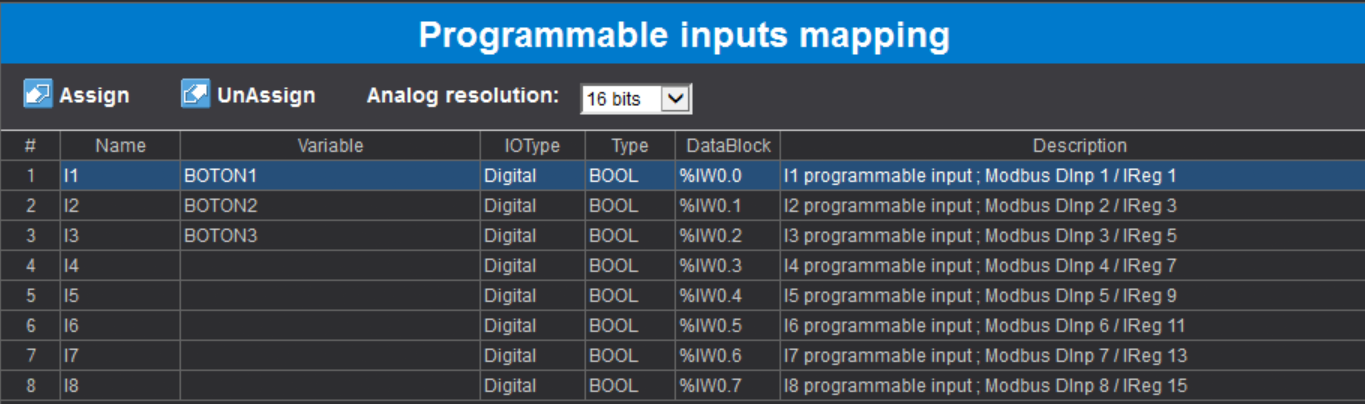
\includegraphics[width=\linewidth]{p2_mapeo_entradas.png}
    \caption{Mapeo de entradas programables: \texttt{BOTON1},
    \texttt{BOTON2} y \texttt{BOTON3} en \texttt{I1}, \texttt{I2} e
    \texttt{I3}.}
    \label{fig:p2_map_in}
\end{figure}

\begin{figure}[H]
    \centering
    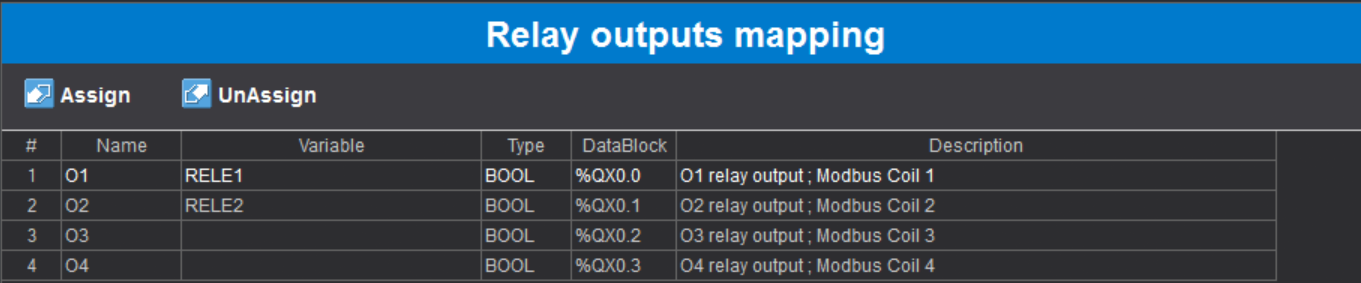
\includegraphics[width=\linewidth]{p2_mapeo_reles.png}
    \caption{Mapeo de salidas de relé: \texttt{RELE1} y \texttt{RELE2} en
    \texttt{O1} y \texttt{O2}.}
    \label{fig:p2_map_rel}
\end{figure}

\paragraph{Canales de la expansión A0602}
La expansión tiene su propio nodo en \ui{I/O Expansions}
(figura~\ref{fig:expansion_analogica}). Con doble clic en
\ui{Programmable Channels} se abre la tabla \ui{Programmable channels
mapping} (figura~\ref{fig:p2_canales}). La expansión tiene ocho canales:
seis de entrada (\texttt{I1} a \texttt{I6}) y dos de salida (\texttt{O1} y
\texttt{O2}). La columna \ui{IOType} fija el modo de cada uno. En esta
práctica se usan dos canales, y a cada uno se le asigna su variable con
\ui{Assign}:

\begin{itemize}
    \item \texttt{I1}, en modo \ui{Input - Voltage ADC}, con la variable
    \texttt{TEMP\_RAW} (\texttt{\%IB10.0}). Es la entrada del sensor de
    temperatura. El convertidor es de 16~bits~\cite{a0602}: la variable,
    de tipo \texttt{UINT}, toma valores de 0 a 65535, que corresponden a
    0 a 10~V en el borne.
    \item \texttt{O1}, en modo \ui{Output - Voltage DAC}, con la
    variable \texttt{SALIDA\_EASYPORT}, en la dirección
    \texttt{\%QB10.16}. Es la salida analógica
    que lleva la orden del ventilador al EasyPort, donde se visualiza en
    su pantalla.
\end{itemize}

Los demás canales quedan sin variable. Las columnas \ui{DataBlock} y
\ui{Description} muestran la dirección de cada canal en el PLC y en
Modbus; no hace falta modificarlas.

\begin{figure}[H]
    \centering
    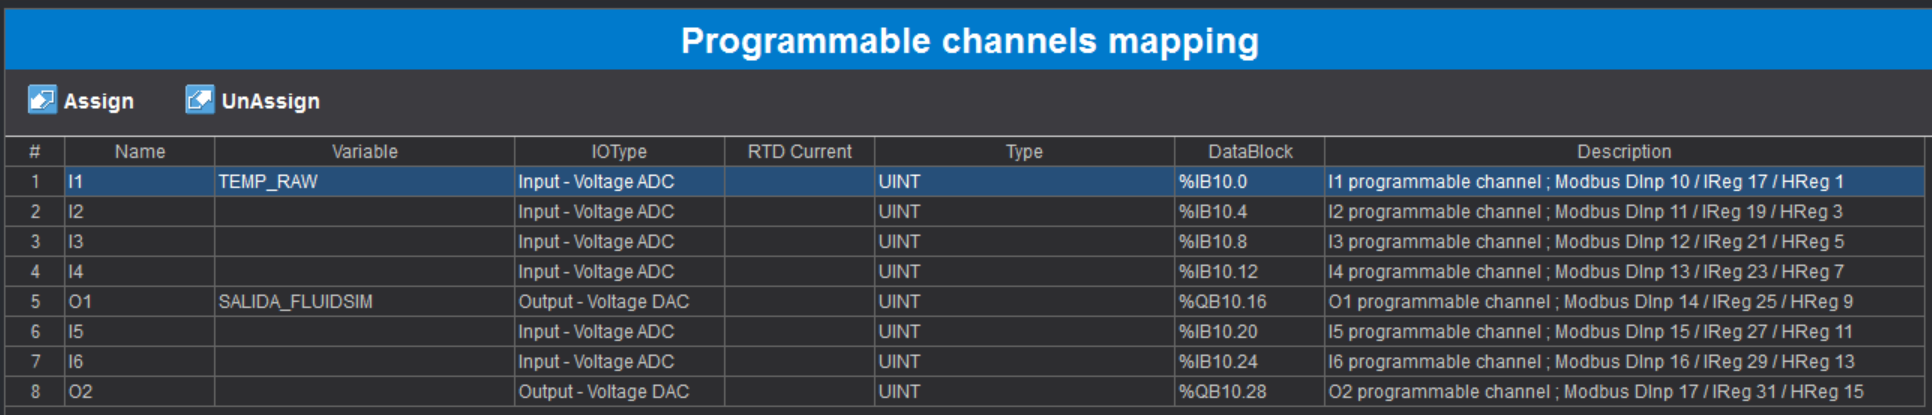
\includegraphics[width=\linewidth]{Mapeo_canales_programables_ejer2.png}
    \caption{Canales programables de la expansión A0602:
    \texttt{TEMP\_RAW} en el canal \texttt{I1} (\ui{Input - Voltage ADC})
    y \texttt{SALIDA\_EASYPORT} en el canal \texttt{O1}
    (\ui{Output - Voltage DAC}).}
    \label{fig:p2_canales}
\end{figure}

\paragraph{Salidas PWM de la expansión}
Con doble clic en \ui{PWM Outputs} se abre la tabla de la
figura~\ref{fig:p2_pwm}. Cada salida PWM tiene dos variables de tipo
\texttt{UDINT}: el periodo (\emph{PERIOD}) y el ancho del pulso
(\emph{PULSE}). El ciclo útil es el cociente \emph{PULSE}/\emph{PERIOD}. Se
asignan \texttt{MOTOR\_PERIODO} a \ui{P1 PERIOD} y \texttt{MOTOR\_PULSO} a
\ui{P1 PULSE}.

\begin{figure}[H]
    \centering
    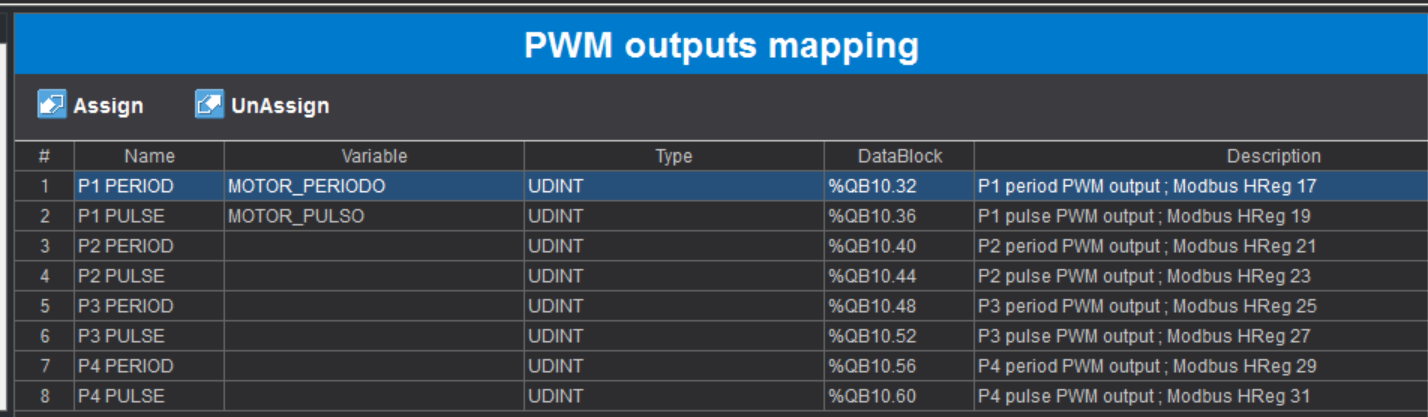
\includegraphics[width=\linewidth]{p2_pwm_mapeo.png}
    \caption{Mapeo de las salidas PWM: \texttt{MOTOR\_PERIODO} y
    \texttt{MOTOR\_PULSO} en \texttt{P1}.}
    \label{fig:p2_pwm}
\end{figure}

\begin{nota}
La tabla del PLC IDE no indica la unidad del periodo, y el manual de la
expansión solo dice que el periodo es programable~\cite{a0602}. El
tutorial de Arduino aclara que \emph{PERIOD} y \emph{PULSE} se expresan en
microsegundos~\cite{optaanalogtut}: con un periodo de \texttt{1000}, la
señal tiene un periodo de 1~ms, es decir, 1~kHz. El ciclo útil no depende
de la unidad, solo del cociente \emph{PULSE}/\emph{PERIOD}.
\end{nota}

\paragraph{Variables locales}
Las variables que el programa usa solo en su interior se declaran en la
tabla \ui{Local variables} del programa (columnas \ui{Name}, \ui{Type},
\ui{Address}, \ui{Array}, \ui{Init value}). Con \ui{Address} en
\texttt{Auto} y \ui{Array} en \texttt{No}, el IDE se encarga del resto.
El programa usa 34 variables locales. La figura~\ref{fig:p2_vars} muestra
cómo quedan declaradas en el IDE, con sus valores iniciales: la tabla es
más larga que la ventana, así que la captura se divide en dos partes (filas
1 a 32 y filas 33 y 34). La tabla~\ref{tab:p2_vars} explica para qué sirve
cada una. Las variables ligadas a hardware
(\texttt{BOTON1} a \texttt{BOTON3}, \texttt{RELE1}, \texttt{RELE2},
\texttt{TEMP\_RAW}, \texttt{SALIDA\_EASYPORT}, \texttt{MOTOR\_PERIODO} y
\texttt{MOTOR\_PULSO}) son globales: las crea el mapeo y no se declaran
aquí.

\begin{advertencia}
Declarar cada variable local \emph{antes} de escribirla en un contacto, una
bobina o un bloque. Si se teclea un nombre que no existe, el editor lo crea
como variable global y, al compilar, aparecen errores como
\texttt{A4097 Object not found} o el aviso \texttt{G0295} por variable
duplicada. Si ocurre, borrar la copia errónea del nodo en que se creó (en
este proyecto apareció en \texttt{I\_O\_mappings\_ProgInp}) y declararla
correctamente en \ui{Local variables}.
\end{advertencia}

\begin{figure}[H]
    \centering
    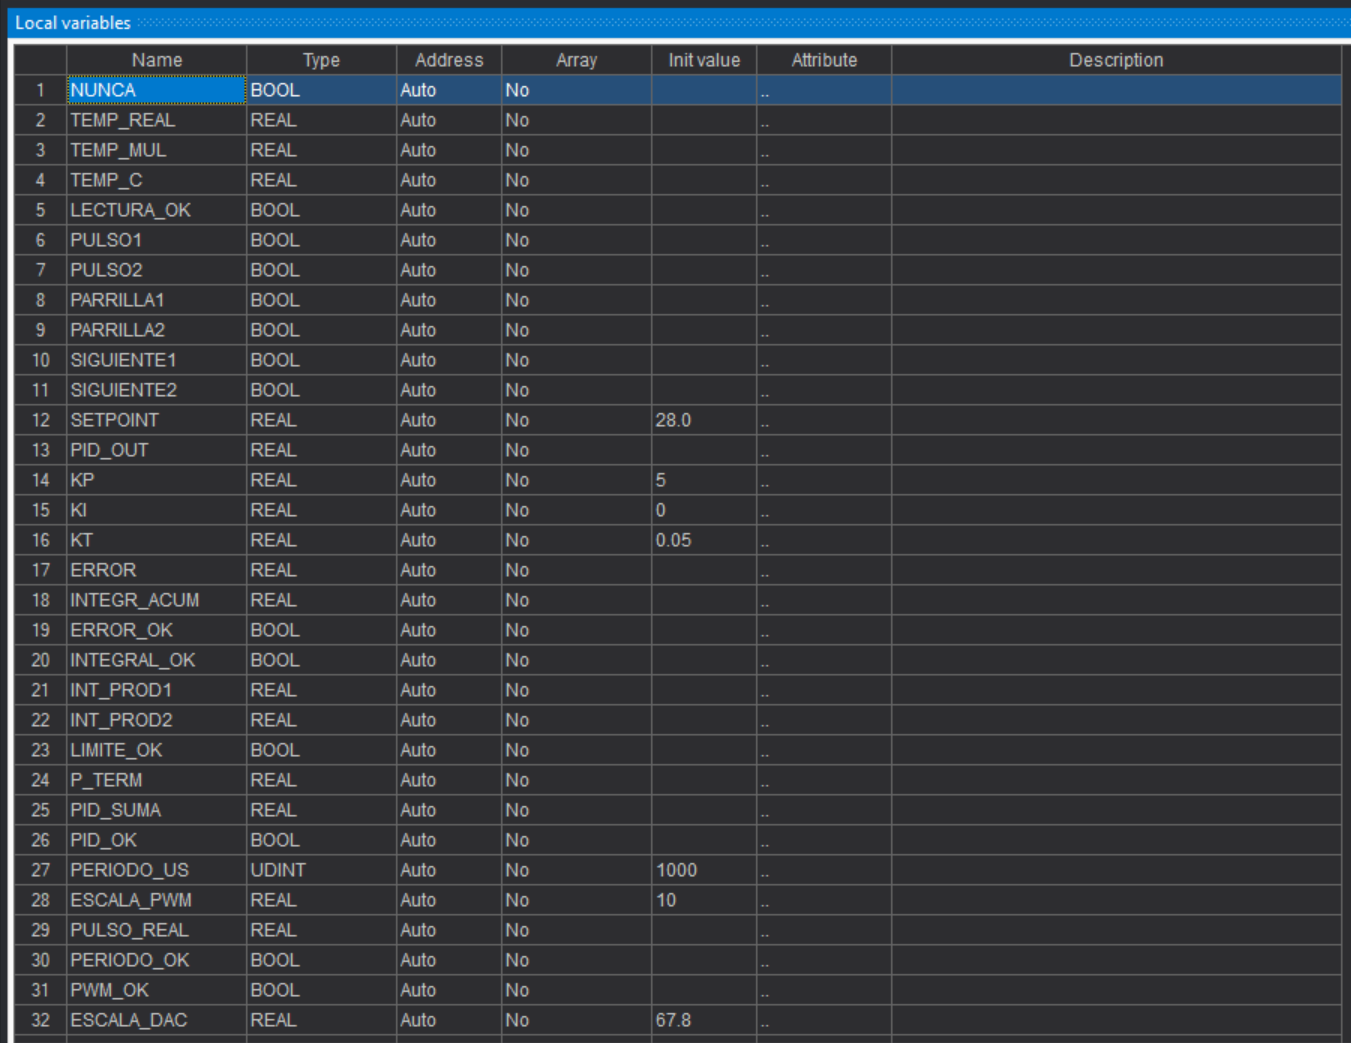
\includegraphics[width=0.85\linewidth]{variables_locales_1_ejer2.png}\\[2pt]
    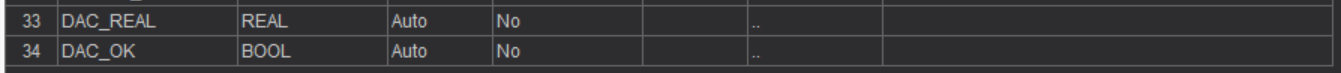
\includegraphics[width=0.85\linewidth]{variables_locales_2_ejer2.png}
    \caption{Tabla \ui{Local variables} del programa: las 34 variables
    locales con sus valores iniciales (filas 1 a 32 arriba, 33 y 34
    abajo).}
    \label{fig:p2_vars}
\end{figure}

\begin{table}[H]
\centering
\caption{Variables locales del programa
\texttt{Sistema\_\allowbreak de\_\allowbreak enfriamiento}. Fuente: Autora.}
\label{tab:p2_vars}
\linespread{1}\small\selectfont
\renewcommand{\arraystretch}{1.1}
\begin{tabularx}{\linewidth}{l l l X}
\toprule
\textbf{Variable} & \textbf{Tipo} & \textbf{Valor inicial} & \textbf{Función} \\
\midrule
\texttt{NUNCA}                      & BOOL  &                  & Nunca se activa; su contacto negado deja la línea siempre cerrada (habilita los bloques) \\
\texttt{PULSO1}, \texttt{PULSO2}    & BOOL  &                  & Pulso de un ciclo al presionar \texttt{BOTON1} o \texttt{BOTON2} \\
\texttt{SIGUIENTE1}, \texttt{SIGUIENTE2} & BOOL &               & Siguiente estado de cada parrilla antes del paro \\
\texttt{PARRILLA1}, \texttt{PARRILLA2} & BOOL &                 & Estado de cada calentador (alimentan \texttt{RELE1} y \texttt{RELE2}) \\
\texttt{TEMP\_REAL}                 & REAL  &                  & \texttt{TEMP\_RAW} convertido a real \\
\texttt{TEMP\_MUL}                  & REAL  &                  & \texttt{TEMP\_REAL} multiplicado por la pendiente \\
\texttt{TEMP\_C}                    & REAL  &                  & Temperatura en $^\circ$C \\
\texttt{LECTURA\_OK}                & BOOL  &                  & Indica que la cadena de lectura terminó \\
\texttt{SETPOINT}                   & REAL  & \texttt{28.0}    & Temperatura deseada \\
\texttt{KP}                         & REAL  & \texttt{5}       & Ganancia proporcional \\
\texttt{KI}                         & REAL  & \texttt{0}       & Ganancia integral (sin efecto con 0) \\
\texttt{KT}                         & REAL  & \texttt{0.05}    & Periodo de la tarea en segundos (50~ms) \\
\texttt{ERROR}                      & REAL  &                  & \texttt{TEMP\_C} $-$ \texttt{SETPOINT} \\
\texttt{ERROR\_OK}                  & BOOL  &                  & Indica que se calculó el error \\
\texttt{INT\_PROD1}, \texttt{INT\_PROD2} & REAL &                & Productos intermedios de la integral \\
\texttt{INTEGR\_ACUM}               & REAL  &                  & Acumulador de la integral \\
\texttt{INTEGRAL\_OK}, \texttt{LIMITE\_OK} & BOOL &              & Confirmaciones de las Redes 0011 y 0012 \\
\texttt{P\_TERM}                    & REAL  &                  & Término proporcional \texttt{ERROR} $\times$ \texttt{KP} \\
\texttt{PID\_SUMA}                  & REAL  &                  & \texttt{P\_TERM} + \texttt{INTEGR\_ACUM}, sin limitar \\
\texttt{PID\_OUT}                   & REAL  &                  & Salida del controlador, limitada a 0--100~\% \\
\texttt{PID\_OK}                    & BOOL  &                  & Indica que se calculó la salida \\
\texttt{PERIODO\_US}                & UDINT & \texttt{1000}    & Periodo del PWM, en $\mu$s \\
\texttt{ESCALA\_PWM}                & REAL  & \texttt{10}      & Convierte 0--100~\% en ancho de pulso (\texttt{PERIODO\_US}/100) \\
\texttt{PULSO\_REAL}                & REAL  &                  & Ancho de pulso calculado, antes de convertirlo a entero \\
\texttt{PERIODO\_OK}, \texttt{PWM\_OK} & BOOL &                  & Confirmaciones de las Redes 0014 y 0015 \\
\texttt{ESCALA\_DAC}                & REAL  & \texttt{67.8}    & Convierte 0--100~\% en cuentas del DAC (medido, ver Red~0016) \\
\texttt{DAC\_REAL}                  & REAL  &                  & Valor del DAC calculado, antes de convertirlo a entero \\
\texttt{DAC\_OK}                    & BOOL  &                  & Confirmación de la Red 0016 \\
\bottomrule
\end{tabularx}
\end{table}

\paragraph{Resumen del mapeo}
La tabla~\ref{tab:p2_mapeo} reúne todos los canales mapeados en esta
sección: entradas y salidas de relé del Opta, canales programables de la
expansión y salidas PWM, con la variable, el tipo y la dirección de cada
uno.

\begin{table}[H]
\centering
\caption{Mapeo de entradas y salidas usado en este ejercicio. Fuente: Autora.}
\label{tab:p2_mapeo}
\linespread{1}\small\selectfont
\renewcommand{\arraystretch}{1.2}
\begin{tabularx}{\linewidth}{l l l l X}
\toprule
\textbf{Canal} & \textbf{Variable} & \textbf{Tipo} & \textbf{Dirección} & \textbf{Significado} \\
\midrule
\multicolumn{5}{l}{\textit{Opta, \ui{Programmable Inputs}}} \\
\midrule
\texttt{I1} & \texttt{BOTON1} & BOOL & \texttt{\%IW0.0} & Pulsador~1: alterna la parrilla~1 \\
\texttt{I2} & \texttt{BOTON2} & BOOL & \texttt{\%IW0.1} & Pulsador~2: alterna la parrilla~2 \\
\texttt{I3} & \texttt{BOTON3} & BOOL & \texttt{\%IW0.2} & Pulsador~3: apaga las dos parrillas \\
\midrule
\multicolumn{5}{l}{\textit{Opta, \ui{Relay Outputs}}} \\
\midrule
\texttt{O1} & \texttt{RELE1} & BOOL & \texttt{\%QX0.0} & Calentador izquierdo (parrilla~1) \\
\texttt{O2} & \texttt{RELE2} & BOOL & \texttt{\%QX0.1} & Calentador derecho (parrilla~2) \\
\midrule
\multicolumn{5}{l}{\textit{A0602, \ui{Programmable Channels}}} \\
\midrule
\texttt{I1} & \texttt{TEMP\_RAW} & UINT & \texttt{\%IB10.0} & Tensión del sensor, 0 a 65\,535 cuentas \\
\texttt{O1} & \texttt{SALIDA\_EASYPORT} & UINT & \texttt{\%QB10.16} & Orden del ventilador en 0--10~V, hacia el EasyPort \\
\midrule
\multicolumn{5}{l}{\textit{A0602, \ui{PWM Outputs}}} \\
\midrule
\texttt{P1 PERIOD} & \texttt{MOTOR\_PERIODO} & UDINT & \texttt{\%QB10.32} & Periodo del PWM del motor \\
\texttt{P1 PULSE}  & \texttt{MOTOR\_PULSO}   & UDINT & \texttt{\%QB10.36} & Ancho del pulso del PWM del motor \\
\bottomrule
\end{tabularx}
\end{table}

% -------------------------------------------------
\subsubsection{Programación en Ladder Diagram}
\label{subsubsec:p2_ladder}

El programa tiene dieciséis redes: las ocho primeras manejan los
pulsadores y las parrillas (las cargas térmicas del recinto), las cinco
siguientes leen la temperatura y calculan el control, y las tres últimas
escriben la orden del ventilador en el PWM y en la salida analógica. Contactos, bobinas, contactos negados y ramas en
paralelo se insertan como en la sección~\ref{subsubsec:p1_ladder}.

\paragraph{Redes 0001 a 0003: alternar la parrilla 1 con un pulsador}
\label{par:p2_red01}
Un pulsador sin enclavamiento entrega 1 mientras se presiona, y un ciclo de
escaneo dura mucho menos que una pulsación. Si la lógica actuara en cada
ciclo, la parrilla cambiaría de estado decenas de veces por pulsación. Por
eso la Red 0001 detecta el flanco ascendente: con clic derecho sobre el
contacto $\to$ \ui{Positive contact} (símbolo \texttt{P}) se obtiene un
contacto que vale 1 solo durante un ciclo, en el instante en que
\texttt{BOTON1} pasa de 0 a 1. Su bobina es \texttt{PULSO1}
(figura~\ref{fig:p2_red01}).

\begin{figure}[H]
    \centering
    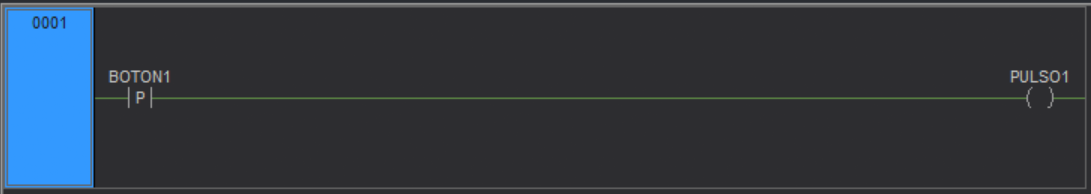
\includegraphics[width=\linewidth]{p2_red01.png}
    \caption{Red 0001: el contacto de flanco ascendente \texttt{BOTON1}
    activa \texttt{PULSO1} durante un ciclo.}
    \label{fig:p2_red01}
\end{figure}

La Red 0002 calcula cómo debe quedar la parrilla. La salida
\texttt{SIGUIENTE1} vale 1 cuando la parrilla y el pulso son distintos:
(PARRILLA1 Y /PULSO1) O (/PARRILLA1 Y PULSO1). Es decir, sin pulso
conserva el estado actual y con pulso lo invierte. Los contactos negados se
obtienen con clic derecho $\to$ \ui{Negate contact}, y la rama inferior con
clic derecho $\to$ \ui{New Parallel contact}
(figura~\ref{fig:p2_red02}).

\begin{figure}[H]
    \centering
    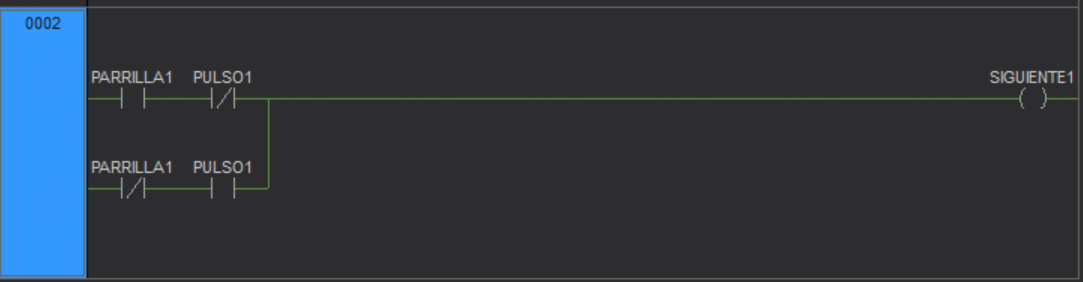
\includegraphics[width=\linewidth]{p2_red02.png}
    \caption{Red 0002: \texttt{SIGUIENTE1} es el estado actual de la
    parrilla, invertido cuando llega el pulso.}
    \label{fig:p2_red02}
\end{figure}

La Red 0003 escribe el resultado en \texttt{PARRILLA1}, salvo que
\texttt{BOTON3} esté presionado: el contacto negado de \texttt{BOTON3}
corta la línea y apaga la parrilla. Separar el cálculo del siguiente estado
de su escritura deja \texttt{PARRILLA1} modificada en un solo lugar del
programa (figura~\ref{fig:p2_red03}).

\begin{figure}[H]
    \centering
    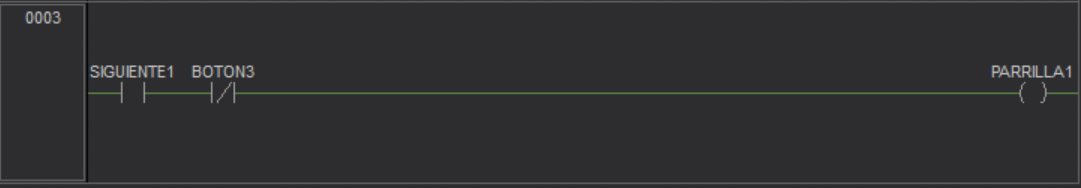
\includegraphics[width=\linewidth]{p2_red03.png}
    \caption{Red 0003: \texttt{PARRILLA1} toma el valor de
    \texttt{SIGUIENTE1} si \texttt{BOTON3} no está presionado.}
    \label{fig:p2_red03}
\end{figure}

\paragraph{Redes 0004 a 0006: la parrilla 2, con el mismo patrón}
Las Redes 0004 a 0006 repiten exactamente las anteriores para la
parrilla~2, con \texttt{BOTON2}, \texttt{PULSO2}, \texttt{SIGUIENTE2} y
\texttt{PARRILLA2}. \texttt{BOTON3} apaga las dos parrillas a la vez
(figura~\ref{fig:p2_red04}).

\begin{figure}[H]
    \centering
    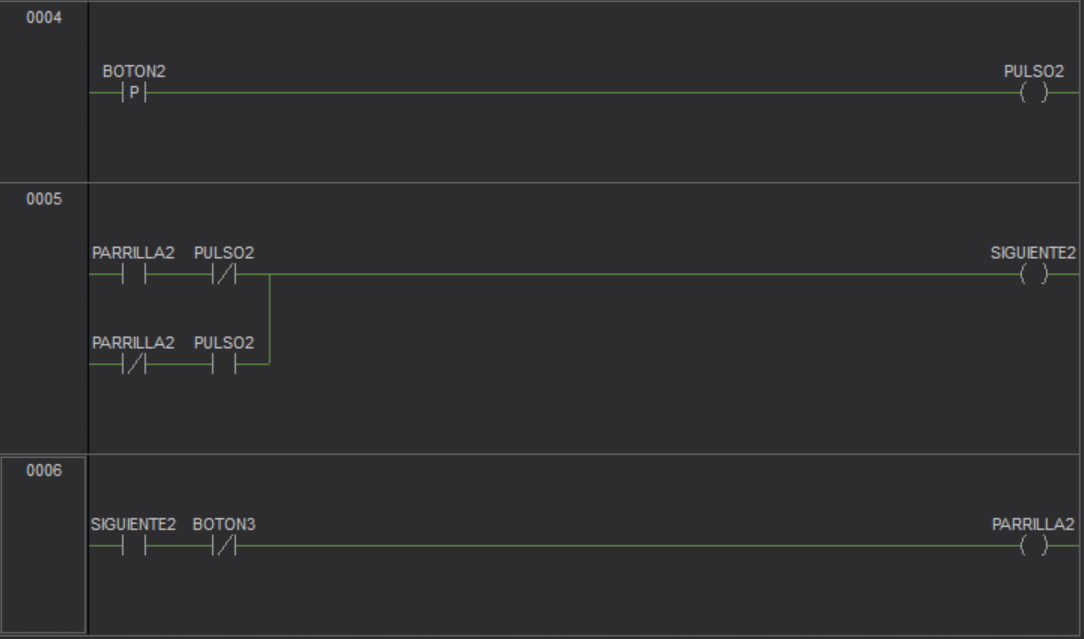
\includegraphics[width=\linewidth]{p2_redes04_06.png}
    \caption{Redes 0004 a 0006: alternancia de la parrilla~2 con
    \texttt{BOTON2}.}
    \label{fig:p2_red04}
\end{figure}

\paragraph{Redes 0007 y 0008: salidas de relé}
Cada estado de parrilla se lleva a su relé: \texttt{PARRILLA1} enciende
\texttt{RELE1} y \texttt{PARRILLA2} enciende \texttt{RELE2}, que alimentan
los calentadores de la DIN Celsius (figura~\ref{fig:p2_red07}). El LED rojo
de cada calentador de la placa también indica su estado.

\begin{figure}[H]
    \centering
    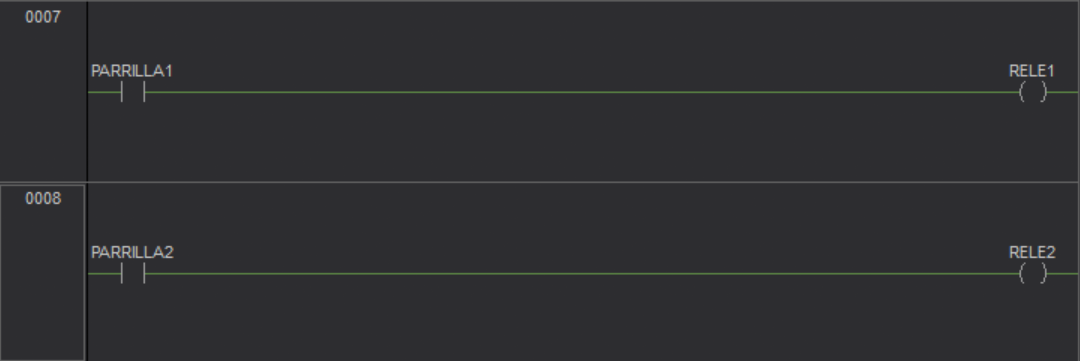
\includegraphics[width=\linewidth]{p2_redes07_08.png}
    \caption{Redes 0007 y 0008: \texttt{PARRILLA1} y \texttt{PARRILLA2}
    activan \texttt{RELE1} y \texttt{RELE2}.}
    \label{fig:p2_red07}
\end{figure}

\paragraph{Red 0009: lectura de temperatura}
\label{par:p2_red09}
Desde esta red el programa usa bloques de función aritméticos. Se
encuentran en \menu{Library Tree}{Operators and blocks}, agrupados en
carpetas como \ui{Arithmetic}, \ui{Conversion}, \ui{Selection} y
\ui{Comparison} (figura~\ref{fig:p2_lib}).

\begin{figure}[H]
    \centering
    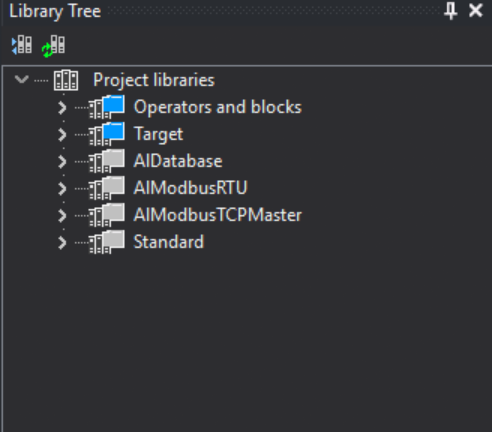
\includegraphics[width=0.4\linewidth]{p2_library_tree.png}
    \caption{Panel \ui{Library Tree}: los operadores y bloques están en
    \ui{Operators and blocks}.}
    \label{fig:p2_lib}
\end{figure}

Los bloques tienen un pin de habilitación \texttt{EN} y una salida
\texttt{ENO} que indica que el bloque se ejecutó. Para que se ejecuten
siempre, en todas las redes de cálculo se aplica la misma técnica:

\begin{itemize}
    \item A la izquierda de la red se coloca el contacto \texttt{NUNCA},
    negado. \texttt{NUNCA} es una variable que ningún lugar del programa
    activa; su contacto negado vale siempre 1 y deja la línea habilitada.
    \item Los bloques se encadenan por \texttt{EN}/\texttt{ENO}, y el
    \texttt{ENO} del último va a una bobina de confirmación
    (\texttt{LECTURA\_OK} en esta red).
    \item Los datos no pasan de un bloque al siguiente por cable, sino por
    variables intermedias con nombre: cada bloque escribe su resultado en
    una variable y el siguiente la lee. Una variable por paso permite ver
    cada resultado en la tabla de observación
    (sección~\ref{subsubsec:p2_verif}).
\end{itemize}

La Red 0009 convierte las cuentas del convertidor analógico en grados
(figura~\ref{fig:p2_red09}):

\begin{enumerate}
    \item \texttt{TO\_REAL} convierte \texttt{TEMP\_RAW} (\texttt{UINT}) en
    \texttt{TEMP\_REAL} (\texttt{REAL}). Los bloques de conversión se
    nombran por el tipo al que convierten (figura~\ref{fig:p2_conv}).
    \item \texttt{MUL} multiplica \texttt{TEMP\_REAL} por
    \texttt{0.0015969} y guarda \texttt{TEMP\_MUL}.
    \item \texttt{SUB} resta \texttt{20.51} de \texttt{TEMP\_MUL} y guarda
    \texttt{TEMP\_C}.
\end{enumerate}

\begin{figure}[H]
    \centering
    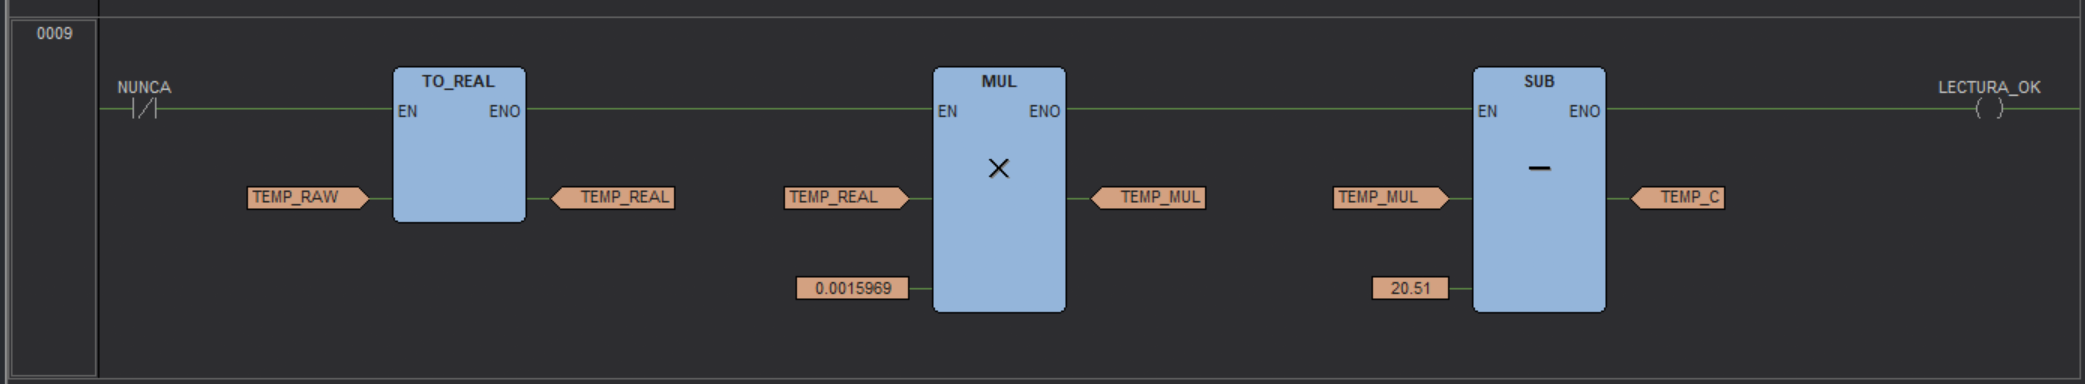
\includegraphics[width=\linewidth]{p2_red09.png}
    \caption{Red 0009: \texttt{TEMP\_RAW} se convierte en \texttt{TEMP\_C}
    con \texttt{TO\_REAL}, \texttt{MUL} y \texttt{SUB}.}
    \label{fig:p2_red09}
\end{figure}

\begin{figure}[H]
    \centering
    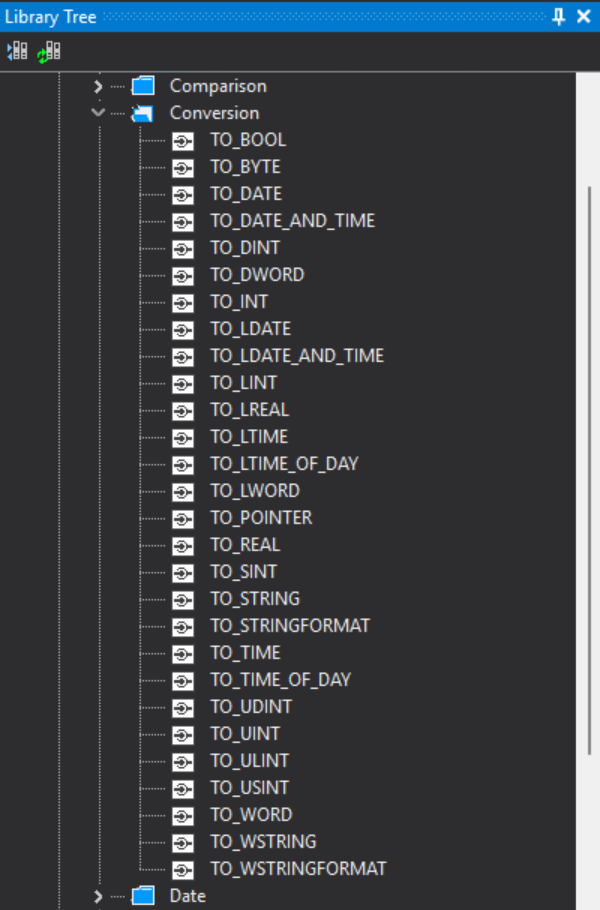
\includegraphics[width=0.4\linewidth]{p2_conversion_blocks.png}
    \caption{Carpeta \ui{Conversion} de \ui{Operators and blocks}: bloques
    \texttt{TO\_*} según el tipo de destino.}
    \label{fig:p2_conv}
\end{figure}

Las constantes \texttt{0.0015969} y \texttt{20.51} salen de los datos del
sensor. El TMP236 entrega 19,5~mV por $^\circ$C y 400~mV a 0~$^\circ$C, y
la placa multiplica esa tensión por 4,9 para obtener una señal de 0 a
10~V~\cite{celsius}. La tensión en el borne es entonces
\[
V = (0{,}4 + 0{,}0195\,T)\cdot 4{,}9 = 1{,}96 + 0{,}09555\,T ,
\]
y el convertidor de 16~bits entrega
$\text{\texttt{TEMP\_RAW}} = V/10 \cdot 65\,535$. Despejando la
temperatura:
\[
T = \text{\texttt{TEMP\_RAW}} \cdot 0{,}0015969 - 20{,}51 .
\]

Con esta fórmula el rango legible llega hasta unos 84~$^\circ$C, donde la
tensión alcanza los 10~V y el convertidor se satura. La
tabla~\ref{tab:p2_calibracion} compara la fórmula con la tabla del
fabricante, que da la tensión redondeada a un decimal.

\begin{table}[H]
\centering
\caption{Comprobación de la conversión con los datos del
fabricante~\cite{celsius}. Fuente: Autora.}
\label{tab:p2_calibracion}
\renewcommand{\arraystretch}{1.3}
\begin{tabular}{c c c c c}
\toprule
\textbf{Temp.\ [$^\circ$C]} & \textbf{Fabricante [V]} & \textbf{Calculada [V]} & \textbf{\texttt{TEMP\_RAW}} & \textbf{\texttt{TEMP\_C} [$^\circ$C]} \\
\midrule
0  & 2,0 & 1,96 & 12\,845 & 0,00 \\
25 & 4,4 & 4,35 & 28\,500 & 25,00 \\
40 & 5,8 & 5,78 & 37\,892 & 40,00 \\
60 & 7,7 & 7,69 & 50\,416 & 60,00 \\
\bottomrule
\end{tabular}
\end{table}

Si la placa está a temperatura ambiente, \texttt{TEMP\_C} debe leer un
valor razonable (en las pruebas de la autora, entre 26 y 29~$^\circ$C). La
figura~\ref{fig:p2_watch_a} muestra la lectura en línea con las dos
parrillas encendidas, y la figura~\ref{fig:p2_watch_b} con ambas apagadas
mientras la placa se enfría.

\begin{figure}[H]
    \centering
    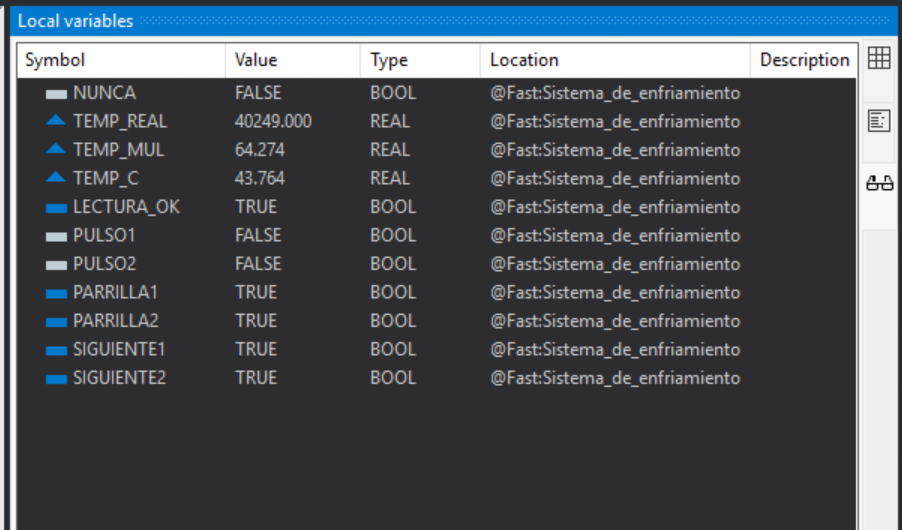
\includegraphics[width=0.75\linewidth]{p2_watch_temp_a.png}
    \caption{Tabla de observación en línea con las parrillas encendidas:
    \texttt{TEMP\_REAL}~=~40\,249 corresponde a
    \texttt{TEMP\_C}~=~43,764~$^\circ$C.}
    \label{fig:p2_watch_a}
\end{figure}

\begin{figure}[H]
    \centering
    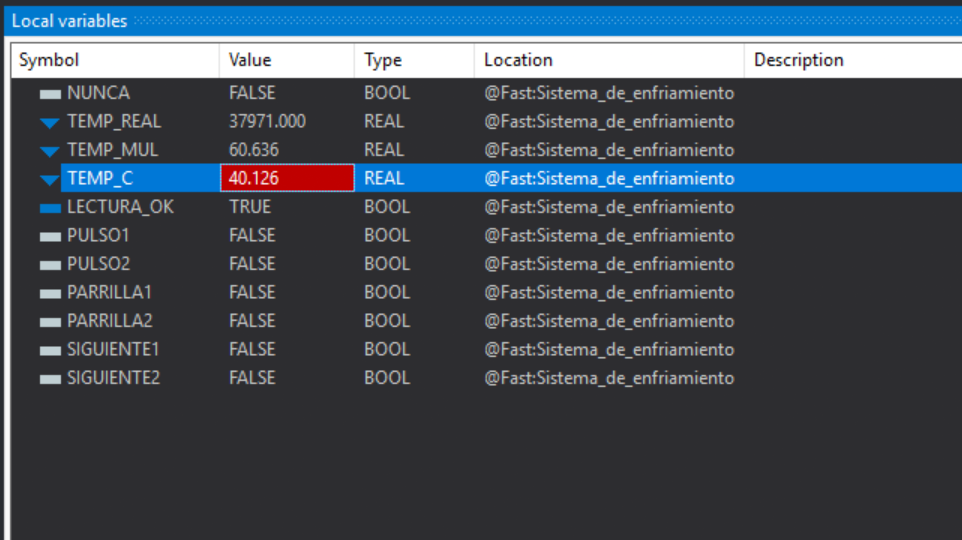
\includegraphics[width=0.75\linewidth]{p2_watch_temp_b.png}
    \caption{Lectura con las parrillas apagadas mientras la placa se
    enfría: \texttt{TEMP\_REAL}~=~37\,971 y
    \texttt{TEMP\_C}~=~40,126~$^\circ$C.}
    \label{fig:p2_watch_b}
\end{figure}

\paragraph{Red 0010: error}
El error es la diferencia entre la temperatura medida y la deseada:
\texttt{SUB} resta \texttt{SETPOINT} de \texttt{TEMP\_C} y guarda
\texttt{ERROR}; la bobina \texttt{ERROR\_OK} confirma la operación
(figura~\ref{fig:p2_red10}). Con la placa más caliente que
\texttt{SETPOINT} el error es positivo y el motor debe girar; con la placa
más fría, es negativo.

\begin{figure}[H]
    \centering
    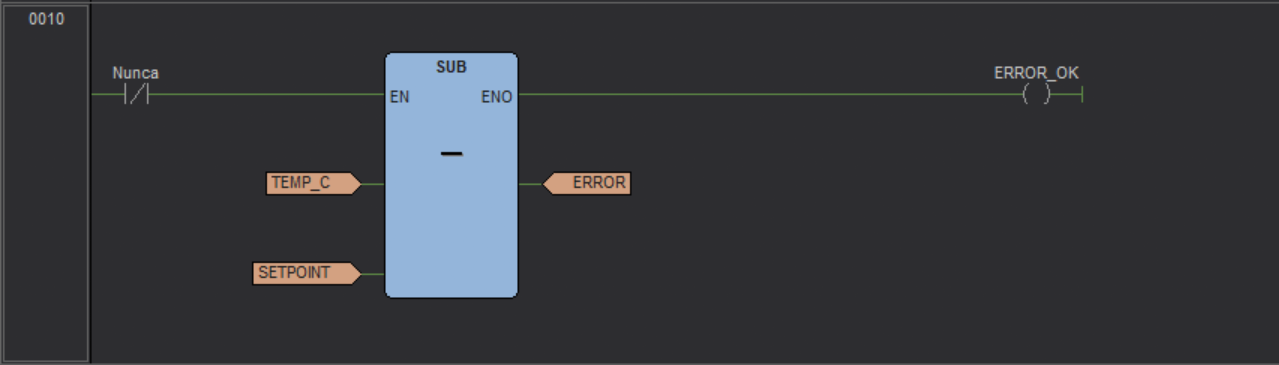
\includegraphics[width=0.85\linewidth]{p2_red10.png}
    \caption{Red 0010: \texttt{ERROR}~=~\texttt{TEMP\_C}~$-$~\texttt{SETPOINT}.}
    \label{fig:p2_red10}
\end{figure}

\paragraph{Redes 0011 y 0012: acción integral (desactivada)}
\label{par:p2_red11}
El PLC IDE de la autora no trae un bloque PID, por lo que el control se
arma con bloques aritméticos. La Red 0011 calcula el incremento de la
integral y lo suma al acumulador (figura~\ref{fig:p2_red11}):

\begin{enumerate}
    \item \texttt{MUL}: \texttt{ERROR} $\times$ \texttt{KI} $\to$
    \texttt{INT\_PROD1}.
    \item \texttt{MUL}: \texttt{KT} $\times$ \texttt{INT\_PROD1} $\to$
    \texttt{INT\_PROD2}. Multiplicar por el periodo de la tarea (0,05~s)
    convierte la suma en una integral.
    \item \texttt{ADD}: \texttt{INTEGR\_ACUM} + \texttt{INT\_PROD2} $\to$
    \texttt{INTEGR\_ACUM}. La variable se suma a sí misma en cada ciclo.
\end{enumerate}

La bobina \texttt{INTEGRAL\_OK} confirma la red. Los pines de un bloque
solo reciben variables o constantes, no la salida de otro bloque; por eso
existen las variables intermedias \texttt{INT\_PROD1} e
\texttt{INT\_PROD2}.

\begin{figure}[H]
    \centering
    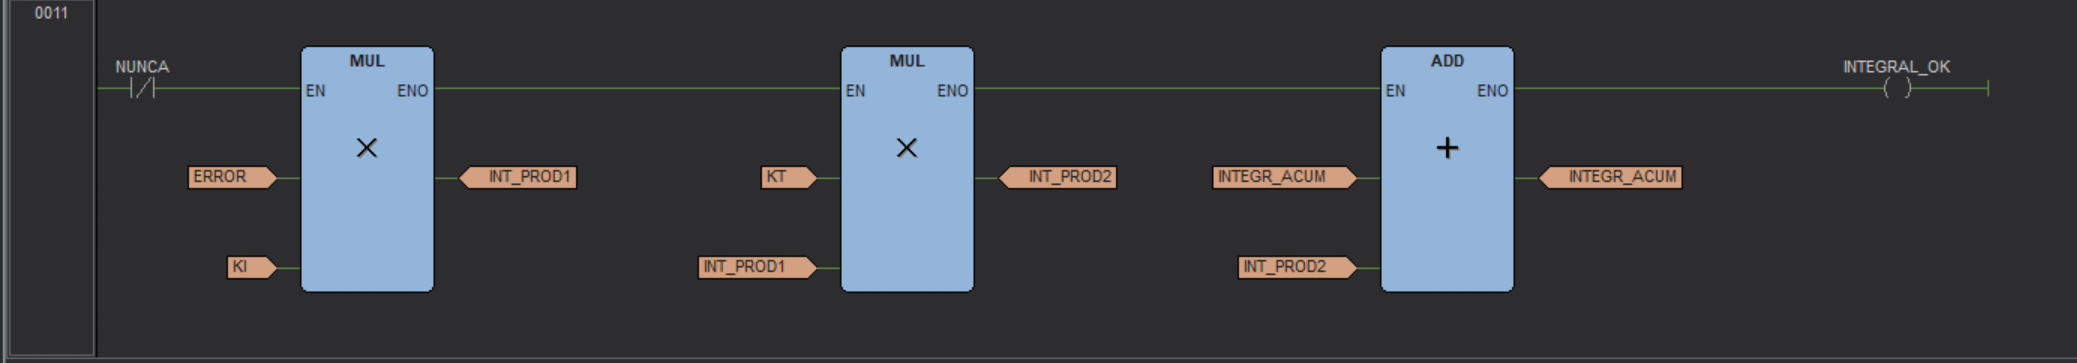
\includegraphics[width=\linewidth]{p2_red11.png}
    \caption{Red 0011: incremento de la integral y acumulación en
    \texttt{INTEGR\_ACUM}.}
    \label{fig:p2_red11}
\end{figure}

La Red 0012 limita el acumulador entre 0 y 100 con el bloque
\texttt{LIMIT} (carpeta \ui{Selection}, figura~\ref{fig:p2_sel}). Sus pines
son \texttt{IN} (el valor a limitar), \texttt{MN} (mínimo) y \texttt{MX}
(máximo). Aquí \texttt{IN} es \texttt{INTEGR\_ACUM}, \texttt{MN} es
\texttt{0.0}, \texttt{MX} es \texttt{100.0} y la salida vuelve a
\texttt{INTEGR\_ACUM}; \texttt{LIMITE\_OK} confirma la red
(figura~\ref{fig:p2_red12}). Limitar el acumulador evita que crezca sin
tope.

\begin{figure}[H]
    \centering
    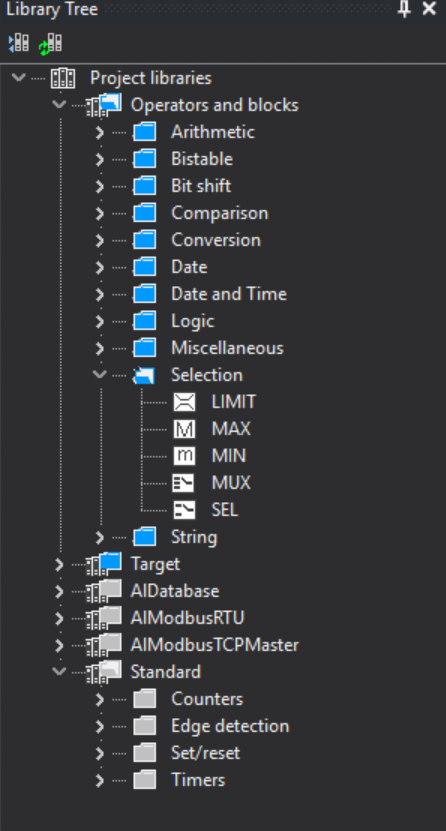
\includegraphics[width=0.4\linewidth]{p2_selection_limit.png}
    \caption{Carpeta \ui{Selection}: \texttt{LIMIT}, \texttt{MAX},
    \texttt{MIN}, \texttt{MUX} y \texttt{SEL}.}
    \label{fig:p2_sel}
\end{figure}

\begin{figure}[H]
    \centering
    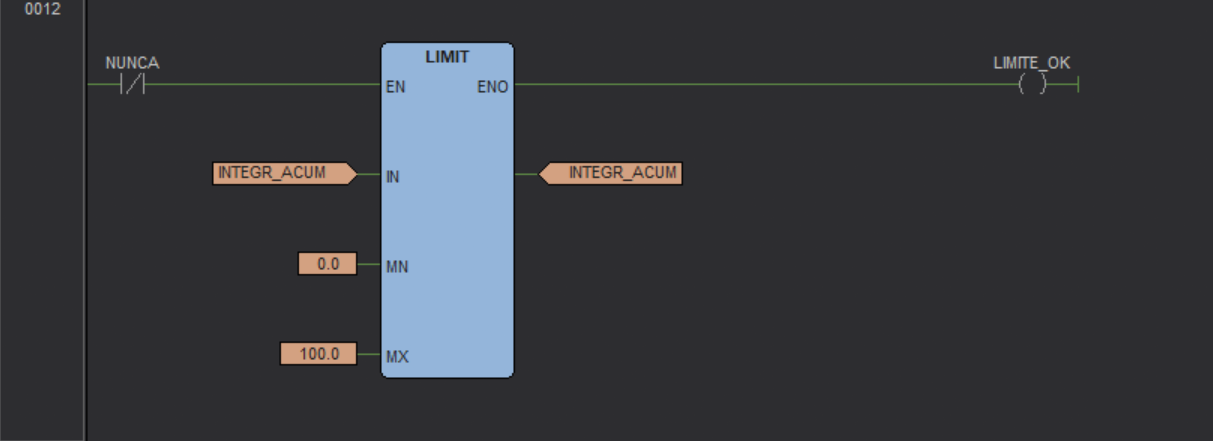
\includegraphics[width=0.85\linewidth]{p2_red12.png}
    \caption{Red 0012: \texttt{LIMIT} mantiene \texttt{INTEGR\_ACUM} entre
    0 y 100.}
    \label{fig:p2_red12}
\end{figure}

\begin{advertencia}
Los límites de \texttt{LIMIT} deben escribirse como números reales:
\texttt{0.0} y \texttt{100.0}. Con enteros (\texttt{0} y \texttt{100}) el
compilador emite el aviso \texttt{G0255} por tipos distintos.
\end{advertencia}

\begin{nota}
Con \texttt{KI}~=~0, \texttt{INT\_PROD1} e \texttt{INT\_PROD2} valen 0 y el
acumulador no cambia. Pero si \texttt{INTEGR\_ACUM} conserva un valor
distinto de 0 de pruebas anteriores (por ejemplo 73,27), se suma a la
salida y la satura: las variables retienen su valor al cambiar
\texttt{KI}, así que hay que ponerlo a 0 en la tabla de observación.
\end{nota}

\paragraph{Red 0013: salida del controlador}
La salida proporcional se calcula en tres pasos
(figura~\ref{fig:p2_red13}):

\begin{enumerate}
    \item \texttt{MUL}: \texttt{ERROR} $\times$ \texttt{KP} $\to$
    \texttt{P\_TERM}.
    \item \texttt{ADD}: \texttt{P\_TERM} + \texttt{INTEGR\_ACUM} $\to$
    \texttt{PID\_SUMA}.
    \item \texttt{LIMIT}: \texttt{PID\_SUMA} entre \texttt{0.0} y
    \texttt{100.0} $\to$ \texttt{PID\_OUT}.
\end{enumerate}

\texttt{PID\_OUT} es el porcentaje de ciclo útil que se pedirá al motor.
Con \texttt{KI}~=~0 equivale a \texttt{KP}~$\cdot$~\texttt{ERROR} acotado a
0--100~\%. La bobina
\texttt{PID\_OK} confirma la red.

\begin{figure}[H]
    \centering
    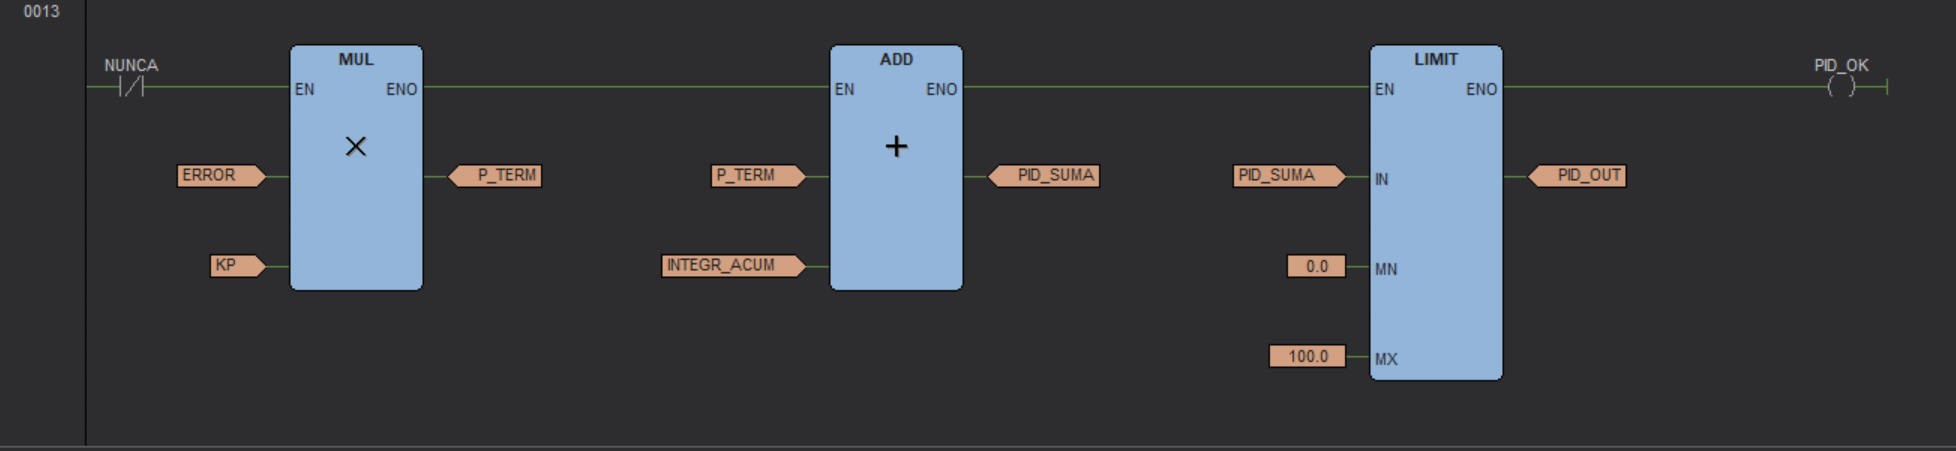
\includegraphics[width=\linewidth]{p2_red13.png}
    \caption{Red 0013: \texttt{PID\_OUT} = \texttt{LIMIT}(\texttt{ERROR}
    $\times$ \texttt{KP} + \texttt{INTEGR\_ACUM}, 0, 100).}
    \label{fig:p2_red13}
\end{figure}

\paragraph{Red 0014: periodo del PWM}
El bloque \texttt{MOVE} copia \texttt{PERIODO\_US} (\texttt{1000}) en
\texttt{MOTOR\_PERIODO}, la variable mapeada al periodo de \texttt{P1}
(figura~\ref{fig:p2_red14}). Se hace en cada ciclo para garantizar que el
periodo esté siempre escrito. \texttt{PERIODO\_OK} confirma la red.

\begin{figure}[H]
    \centering
    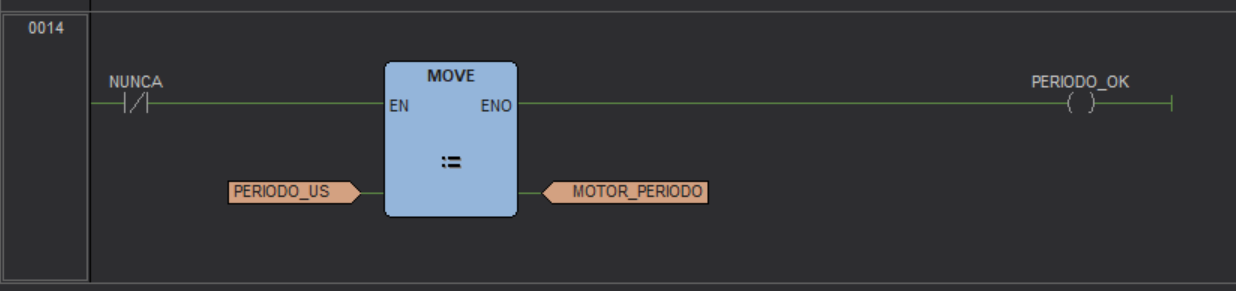
\includegraphics[width=0.85\linewidth]{p2_red14.png}
    \caption{Red 0014: \texttt{MOVE} escribe el periodo en
    \texttt{MOTOR\_PERIODO}.}
    \label{fig:p2_red14}
\end{figure}

\paragraph{Red 0015: ancho de pulso del PWM}
El ciclo útil es \texttt{MOTOR\_PULSO}/\texttt{MOTOR\_PERIODO}. Con el
periodo en 1000, el ancho de pulso para el porcentaje \texttt{PID\_OUT} es
\texttt{PID\_OUT}~$\times$~10. La Red 0015 hace esa operación y entrega un
entero (figura~\ref{fig:p2_red15}):

\begin{enumerate}
    \item \texttt{MUL}: \texttt{PID\_OUT} $\times$ \texttt{ESCALA\_PWM}
    (\texttt{10}) $\to$ \texttt{PULSO\_REAL}.
    \item \texttt{TO\_UDINT}: \texttt{PULSO\_REAL} $\to$
    \texttt{MOTOR\_PULSO}.
\end{enumerate}

La bobina \texttt{PWM\_OK} confirma la red. \texttt{MOTOR\_PULSO} es
\texttt{UDINT}, de modo que el bloque correcto es \texttt{TO\_UDINT}; con
\texttt{TO\_UINT} el tipo de destino no coincide con la variable.

\begin{figure}[H]
    \centering
    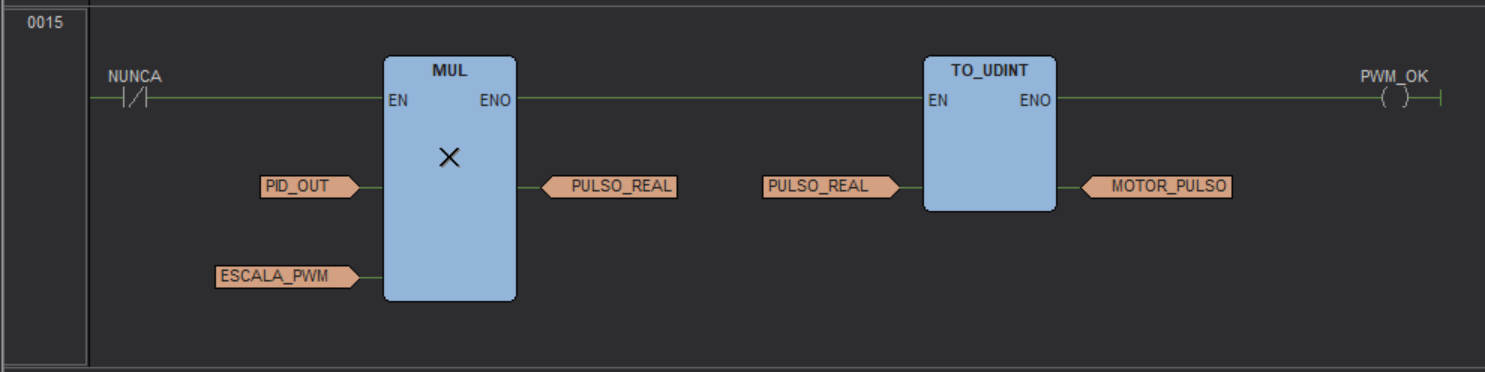
\includegraphics[width=\linewidth]{p2_red15.png}
    \caption{Red 0015: \texttt{PID\_OUT} se escala y se convierte a entero
    para \texttt{MOTOR\_PULSO}.}
    \label{fig:p2_red15}
\end{figure}

La figura~\ref{fig:p2_red1415} muestra las Redes 0014 y 0015 en línea, con
el valor de cada variable sobre sus pines: con \texttt{PID\_OUT}~=~100,
\texttt{MOTOR\_PULSO} vale 1000, igual que el periodo (ciclo útil del
100~\%).

\begin{figure}[H]
    \centering
    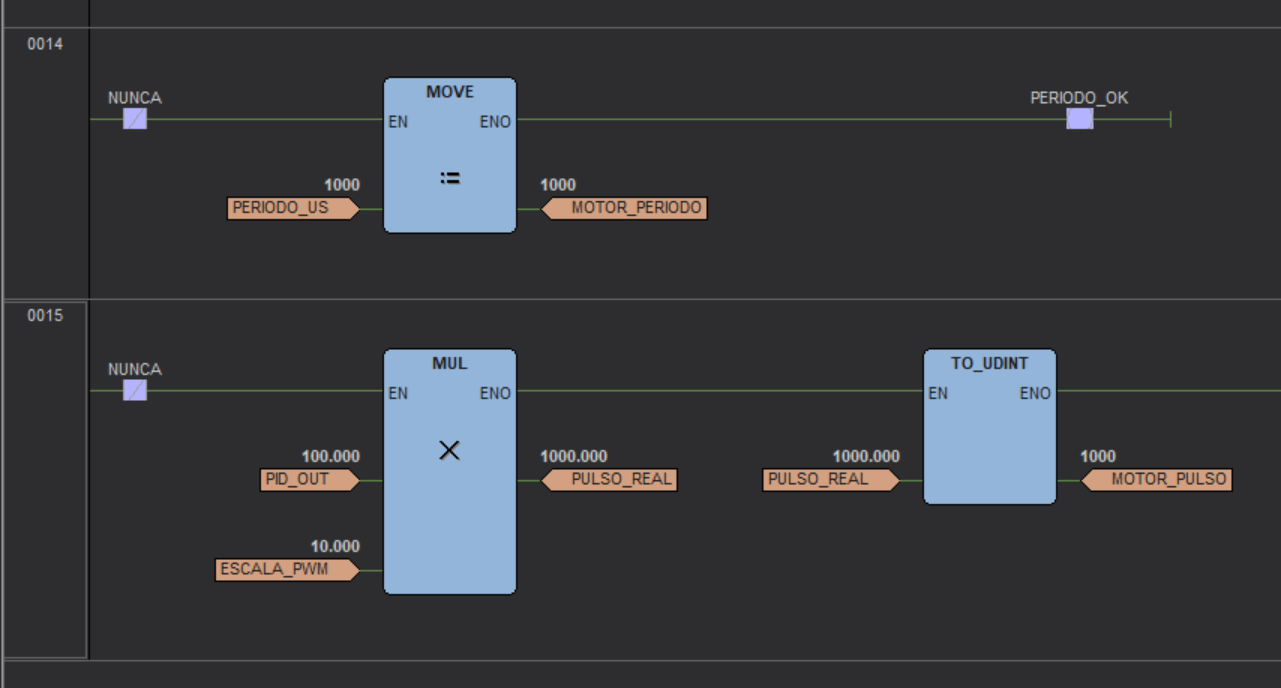
\includegraphics[width=\linewidth]{p2_redes14_15_valores.png}
    \caption{Redes 0014 y 0015 en línea, con los valores de cada variable.}
    \label{fig:p2_red1415}
\end{figure}

\paragraph{Red 0016: salida analógica hacia el EasyPort}
\label{par:p2_red16}
La misma orden del ventilador sale también como tensión por el canal
\texttt{O1} de la expansión, como se haría con la referencia de 0 a 10~V
de un variador de frecuencia. La red sigue el patrón de la Red 0015:

\begin{enumerate}
    \item \texttt{MUL}: \texttt{PID\_OUT} $\times$ \texttt{ESCALA\_DAC}
    $\to$ \texttt{DAC\_REAL}.
    \item \texttt{TO\_UINT}: \texttt{DAC\_REAL} $\to$
    \texttt{SALIDA\_EASYPORT}. Aquí sí corresponde \texttt{TO\_UINT},
    porque \texttt{SALIDA\_EASYPORT} es de tipo \texttt{UINT}.
\end{enumerate}

Como en las demás redes de cálculo, el contacto negado de \texttt{NUNCA}
habilita la línea; el \texttt{ENO} de \texttt{MUL} habilita
\texttt{TO\_UINT}, y el \texttt{ENO} de este activa la bobina
\texttt{DAC\_OK}, que confirma que la red se ejecutó completa
(figura~\ref{fig:p2_red16}). El resultado de la multiplicación no pasa por
cable al segundo bloque: \texttt{MUL} lo escribe en \texttt{DAC\_REAL} y
\texttt{TO\_UINT} lo lee de esa misma variable. La conversión a entero es
necesaria porque el canal del DAC solo acepta un número de cuentas
(\texttt{UINT}), no un real; \texttt{TO\_UINT} descarta los decimales.

\begin{figure}[H]
    \centering
    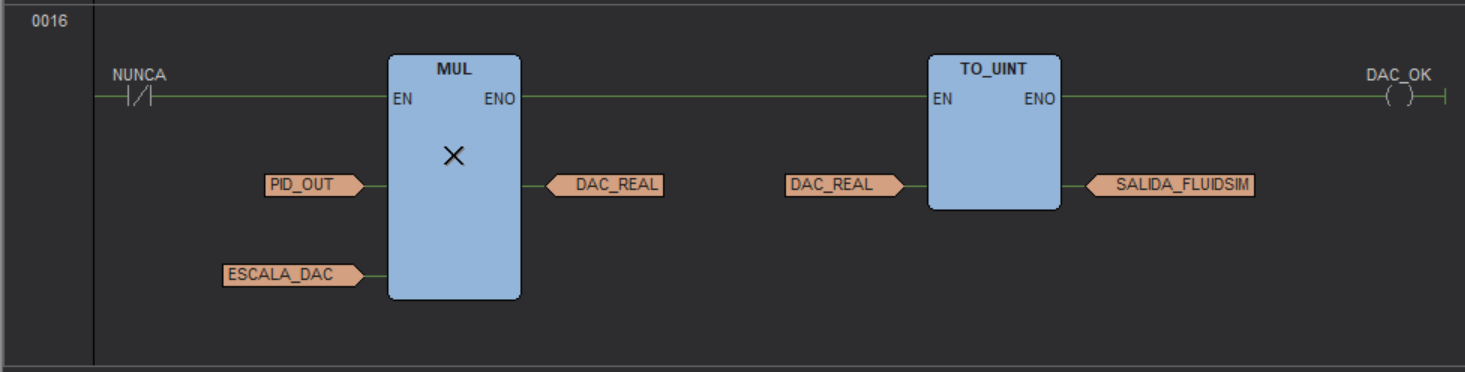
\includegraphics[width=\linewidth]{red16_ejercicio2.png}
    \caption{Red 0016: \texttt{PID\_OUT} se escala con
    \texttt{ESCALA\_DAC} y se convierte a entero para
    \texttt{SALIDA\_EASYPORT}, la salida analógica \texttt{O1} de la
    expansión.}
    \label{fig:p2_red16}
\end{figure}

\texttt{ESCALA\_DAC} es el número de cuentas del DAC que corresponde a
1~\% de \texttt{PID\_OUT}, de modo que con \texttt{PID\_OUT}~=~100 la
salida entregue 10~V. Su valor se obtuvo en el banco: se escribieron
valores fijos en \texttt{SALIDA\_EASYPORT} y se midió con el multímetro la
tensión entre \texttt{O1} y tierra (tabla~\ref{tab:p2_dac}).

\begin{table}[H]
\centering
\caption{Tensión medida en la salida \texttt{O1} para distintos valores de
\texttt{SALIDA\_EASYPORT}. Fuente: Autora.}
\label{tab:p2_dac}
\renewcommand{\arraystretch}{1.2}
\begin{tabular}{c c}
\toprule
\textbf{\texttt{SALIDA\_EASYPORT} [cuentas]} & \textbf{Tensión en \texttt{O1} [V]} \\
\midrule
0     & 0 \\
4000  & 5,9 \\
8000  & 11,8 \\
\bottomrule
\end{tabular}
\end{table}

La relación es una recta que pasa por cero, con una pendiente de
11,8~V~/~8000 = 1,475~mV por cuenta. Para obtener 10~V hacen falta
10~V~/~1,475~mV $\approx$ 6780 cuentas; si el 100~\% de \texttt{PID\_OUT}
debe dar 6780 cuentas, cada 1~\% vale 6780~/~100 = 67,8, que es el valor
inicial de \texttt{ESCALA\_DAC}. La medición también muestra que el DAC
puede entregar más de 10~V (11,8~V con 8000 cuentas): la escala es la que
limita la salida a 10~V, porque \texttt{PID\_OUT} nunca pasa de 100.

Con la red 0016 descargada y el cableado de la
figura~\ref{fig:diagrama_p2}, la tensión de \texttt{O1} llega al EasyPort y
se puede leer de dos maneras: en la pantalla del propio EasyPort, que
muestra el pin~8 como canal~0 de las entradas
(figura~\ref{fig:p2_easyport_pantalla}), o en el computador con el programa Festo
EasyPort Web Bridge, que muestra el mismo pin como \ui{Uin 1}
(figura~\ref{fig:p2_easyport_bridge}). Los demás canales y sus colores
están en la tabla~\ref{tab:cable_analogico}.

\begin{figure}[H]
    \centering
    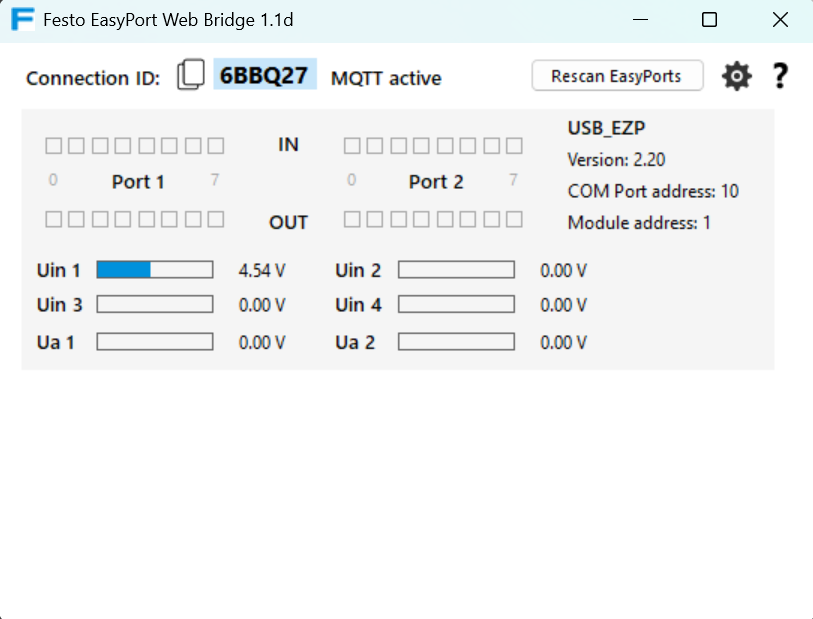
\includegraphics[width=0.7\linewidth,trim=0 117 0 0,clip]{Festo_Easyport_ejemplo2.png}
    \caption{Festo EasyPort Web Bridge con la red 0016 en funcionamiento:
    la tensión de la salida \texttt{O1} de la expansión aparece en
    \ui{Uin 1} (4,54~V en el momento de la captura).}
    \label{fig:p2_easyport_bridge}
\end{figure}

La tabla~\ref{tab:p2_redes} resume las dieciséis redes del programa.

\begin{table}[H]
\centering
\caption{Las dieciséis redes del programa
\texttt{Sistema\_\allowbreak de\_\allowbreak enfriamiento}. Fuente: Autora.}
\label{tab:p2_redes}
\linespread{1}\small\selectfont
\renewcommand{\arraystretch}{1.3}
\begin{tabularx}{\linewidth}{l >{\raggedright\arraybackslash\hyphenpenalty=10000}X >{\raggedright\arraybackslash}p{4.2cm}}
\toprule
\textbf{Red} & \textbf{Lógica} & \textbf{Efecto} \\
\midrule
0001 & BOTON1 (P) $\to$ PULSO1 & Pulso de un ciclo al presionar \texttt{BOTON1} \\
0002 & (PARRILLA1 Y /PULSO1) O (/PARRILLA1 Y PULSO1) $\to$ SIGUIENTE1 & Invierte la parrilla~1 con cada pulso \\
0003 & SIGUIENTE1 Y /BOTON3 $\to$ PARRILLA1 & Actualiza la parrilla~1; \texttt{BOTON3} la apaga \\
0004 & BOTON2 (P) $\to$ PULSO2 & Pulso de un ciclo al presionar \texttt{BOTON2} \\
0005 & (PARRILLA2 Y /PULSO2) O (/PARRILLA2 Y PULSO2) $\to$ SIGUIENTE2 & Invierte la parrilla~2 con cada pulso \\
0006 & SIGUIENTE2 Y /BOTON3 $\to$ PARRILLA2 & Actualiza la parrilla~2; \texttt{BOTON3} la apaga \\
0007 & PARRILLA1 $\to$ RELE1 & Enciende el calentador izquierdo \\
0008 & PARRILLA2 $\to$ RELE2 & Enciende el calentador derecho \\
0009 & \texttt{TO\_REAL}, \texttt{MUL} (0.0015969), \texttt{SUB} (20.51) & \texttt{TEMP\_C} en $^\circ$C \\
0010 & \texttt{SUB}: TEMP\_C $-$ SETPOINT & \texttt{ERROR} \\
0011 & \texttt{MUL}, \texttt{MUL}, \texttt{ADD}: INTEGR\_ACUM += KT $\cdot$ KI $\cdot$ ERROR & Integral (sin efecto con \texttt{KI}~=~0) \\
0012 & \texttt{LIMIT}(INTEGR\_ACUM, 0.0, 100.0) & Acota el acumulador \\
0013 & \texttt{LIMIT}(ERROR $\cdot$ KP + INTEGR\_ACUM, 0.0, 100.0) $\to$ PID\_OUT & Salida del controlador, 0--100~\% \\
0014 & \texttt{MOVE}: PERIODO\_US $\to$ MOTOR\_PERIODO & Periodo del PWM \\
0015 & \texttt{MUL}: PID\_OUT $\cdot$ ESCALA\_PWM; \texttt{TO\_UDINT} $\to$ MOTOR\_PULSO & Velocidad del ventilador (PWM) \\
0016 & \texttt{MUL}: PID\_OUT $\cdot$ ESCALA\_DAC; \texttt{TO\_UINT} $\to$ SALIDA\_EASYPORT & Orden del ventilador en 0--10~V, hacia el EasyPort \\
\bottomrule
\end{tabularx}
\end{table}

% -------------------------------------------------
\subsubsection{Compilación, descarga y verificación en línea}
\label{subsubsec:p2_verif}

El IDE compila el proyecto al guardarlo; la compilación no debe mostrar
errores ni avisos. Después se descarga el programa al Opta.
Con el programa corriendo, la tabla de observación (\ui{Watch}) muestra el
valor de todas las variables.

\begin{advertencia}
Los valores iniciales de la tabla de variables locales se cargan solo al
descargar el programa. Un valor que se cambie a mano en la tabla de
observación (por ejemplo \texttt{SETPOINT}) se pierde en la siguiente
descarga. Si al conectarse una variable muestra 0 y debería tener su valor
inicial (como \texttt{PERIODO\_US}), forzarla en la tabla de observación o
volver a descargar.
\end{advertencia}

Con las parrillas apagadas y la placa a temperatura ambiente, los valores
de la figura~\ref{fig:p2_watch_final} son los esperados:
\texttt{TEMP\_REAL}~=~30\,996 da \texttt{TEMP\_C}~=~28,988~$^\circ$C;
\texttt{ERROR}~=~0,988~$^\circ$C; \texttt{PID\_OUT}~=~4,938~\%;
\texttt{PULSO\_REAL}~=~49,376, es decir, un ciclo útil de
aproximadamente 4,9~\% sobre un periodo de 1000.

\begin{figure}[H]
    \centering
    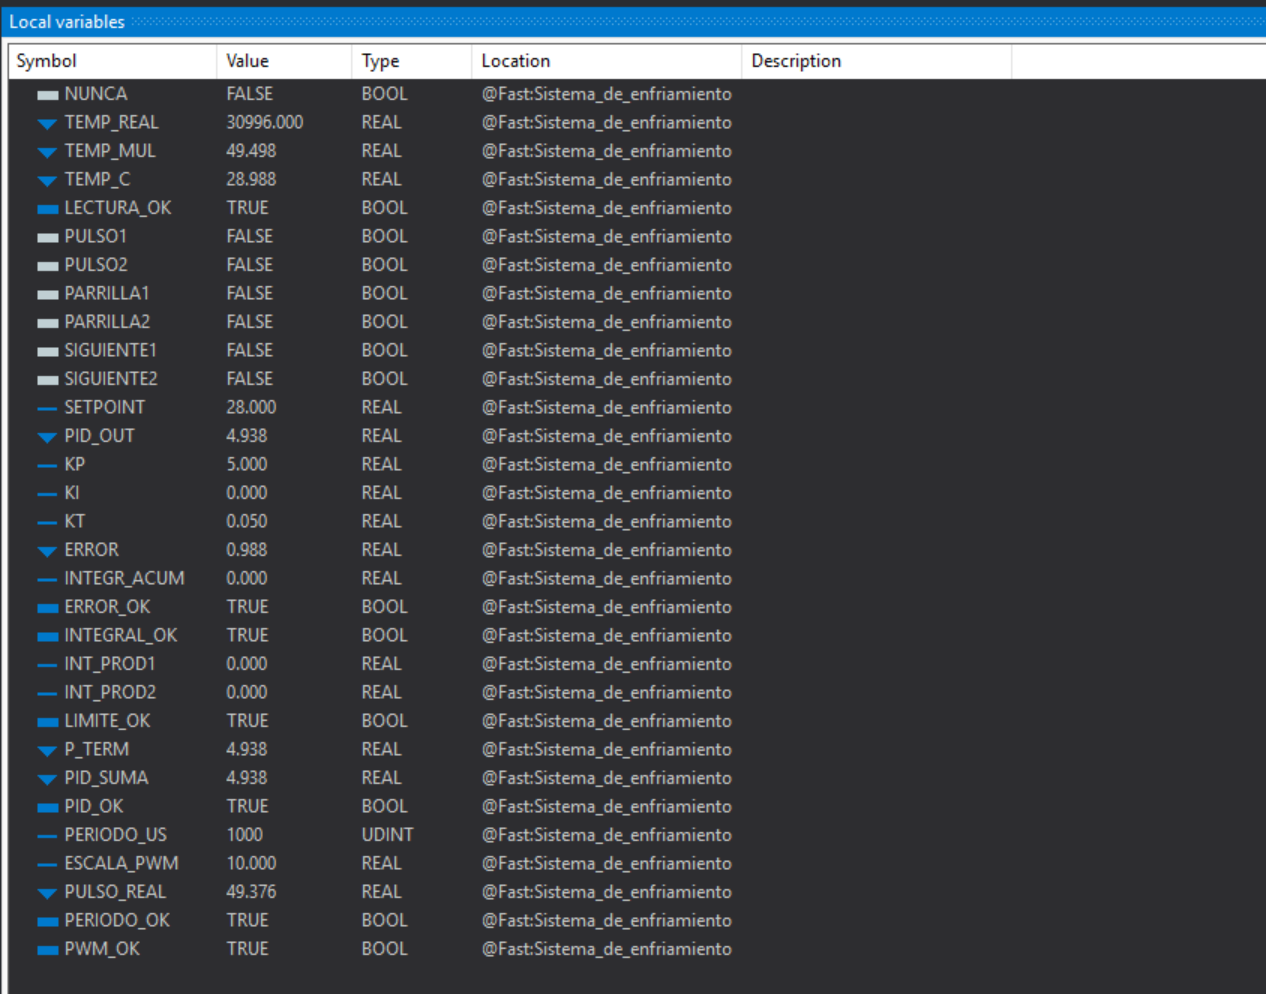
\includegraphics[width=\linewidth]{p2_watch_final.png}
    \caption{Tabla de observación del programa completo, con las parrillas
    apagadas: \texttt{TEMP\_C}~=~28,988~$^\circ$C y
    \texttt{PID\_OUT}~=~4,938~\%.}
    \label{fig:p2_watch_final}
\end{figure}

Para comprobar el lazo se presionan los pulsadores y se observa la tabla:

\begin{enumerate}
    \item Presionar \texttt{BOTON1} y \texttt{BOTON2}: los LED de las
    parrillas se encienden y \texttt{TEMP\_C} empieza a subir.
    \item Al pasar \texttt{TEMP\_C} de 28~$^\circ$C, \texttt{PID\_OUT} sube
    y el motor empieza a girar; a 40~$^\circ$C, \texttt{PID\_OUT} es
    cercano al 60~\%.
    \item Con las dos parrillas encendidas, \texttt{TEMP\_C} llega a
    46--47~$^\circ$C y \texttt{PID\_OUT} a más del 90~\%. Subir
    \texttt{SETPOINT} en la tabla de observación baja \texttt{PID\_OUT} de
    inmediato: con \texttt{SETPOINT}~=~49 y
    \texttt{TEMP\_C}~=~50,3~$^\circ$C, \texttt{PID\_OUT} fue de apenas
    6,5~\%.
    \item Presionar \texttt{BOTON3} apaga las parrillas; \texttt{TEMP\_C}
    baja lentamente y \texttt{PID\_OUT} también.
    \item En todo momento, la tensión entre \texttt{O1} de la expansión y
    tierra, medida con el multímetro, debe ser \texttt{PID\_OUT}/10 en
    voltios: 5~V con \texttt{PID\_OUT}~=~50~\%. La misma tensión se ve en
    el canal~0 de las entradas de la pantalla del EasyPort
    (sección~\ref{subsubsec:p2_pantalla}) y en \ui{Uin 1} de EasyPort
    Web Bridge (figura~\ref{fig:p2_easyport_bridge}).
\end{enumerate}

La tabla~\ref{tab:p2_pruebas} reúne valores medidos y calculados con la
fórmula del programa (\texttt{SETPOINT}~=~28, \texttt{KP}~=~5,
\texttt{KI}~=~0). Diferencias de hasta $\pm$0,01 entre lo medido y lo
calculado son normales, porque la tabla de observación no refresca todas
las variables en el mismo instante.

\begin{table}[H]
\centering
\caption{Valores de comprobación de la cadena \texttt{TEMP\_RAW} $\to$
\texttt{MOTOR\_PULSO}. Fuente: Autora.}
\label{tab:p2_pruebas}
\renewcommand{\arraystretch}{1.3}
\begin{tabular}{c c c c c}
\toprule
\textbf{\texttt{TEMP\_RAW}} & \textbf{\texttt{TEMP\_C} [$^\circ$C]} & \textbf{\texttt{ERROR} [$^\circ$C]} & \textbf{\texttt{PID\_OUT} [\%]} & \textbf{\texttt{PULSO\_REAL}} \\
\midrule
29\,635 & 26,81 & $-$1,19 & 0    & 0 \\
30\,996 & 28,99 & 0,99    & 4,94 & 49,4 \\
33\,996 & 33,78 & 5,78    & 28,9 & 288,9 \\
37\,971 & 40,13 & 12,13   & 60,6 & 606,3 \\
41\,977 & 46,52 & 18,52   & 92,6 & 926,2 \\
44\,762 & 50,97 & 22,97   & 100  & 1000 \\
\bottomrule
\end{tabular}
\end{table}

\begin{nota}
Con un ciclo útil bajo, el motor puede no arrancar: un motor de corriente
continua necesita un mínimo de potencia media para vencer su fricción. Si
el motor se queda detenido con valores bajos de \texttt{PID\_OUT}, es el
comportamiento esperado y no un error del programa.
\end{nota}

\paragraph{Conexiones}
La figura~\ref{fig:diagrama_p2} reúne en un solo diagrama eléctrico el
cableado completo de la práctica. Los pulsadores S1, S2 y S3 del SIMUL8
entran por \texttt{I1}, \texttt{I2} e \texttt{I3} del Opta, y sus relés
\texttt{O1} y \texttt{O2} alimentan los calentadores izquierdo y derecho
de la DIN Celsius. La salida de tensión del sensor llega al borne
\texttt{+I1} de la expansión. El motor queda entre \texttt{P1+} y 0~V; el
borne \texttt{VPWM} recibe +24~V y el borne \texttt{$-$} de ese mismo
grupo va a 0~V. La salida analógica \texttt{+O1} llega al pin~8 (cable
amarillo) del conector analógico de 15 pines del EasyPort, y tanto el
negativo de \texttt{O1} como el pin~6 (0~V, cable gris) del EasyPort se
conectan a la tierra común del Opta. Sin esa tierra compartida, el
EasyPort no tiene una referencia para medir la tensión de \texttt{O1}.

\begin{figure}[H]
    \centering
    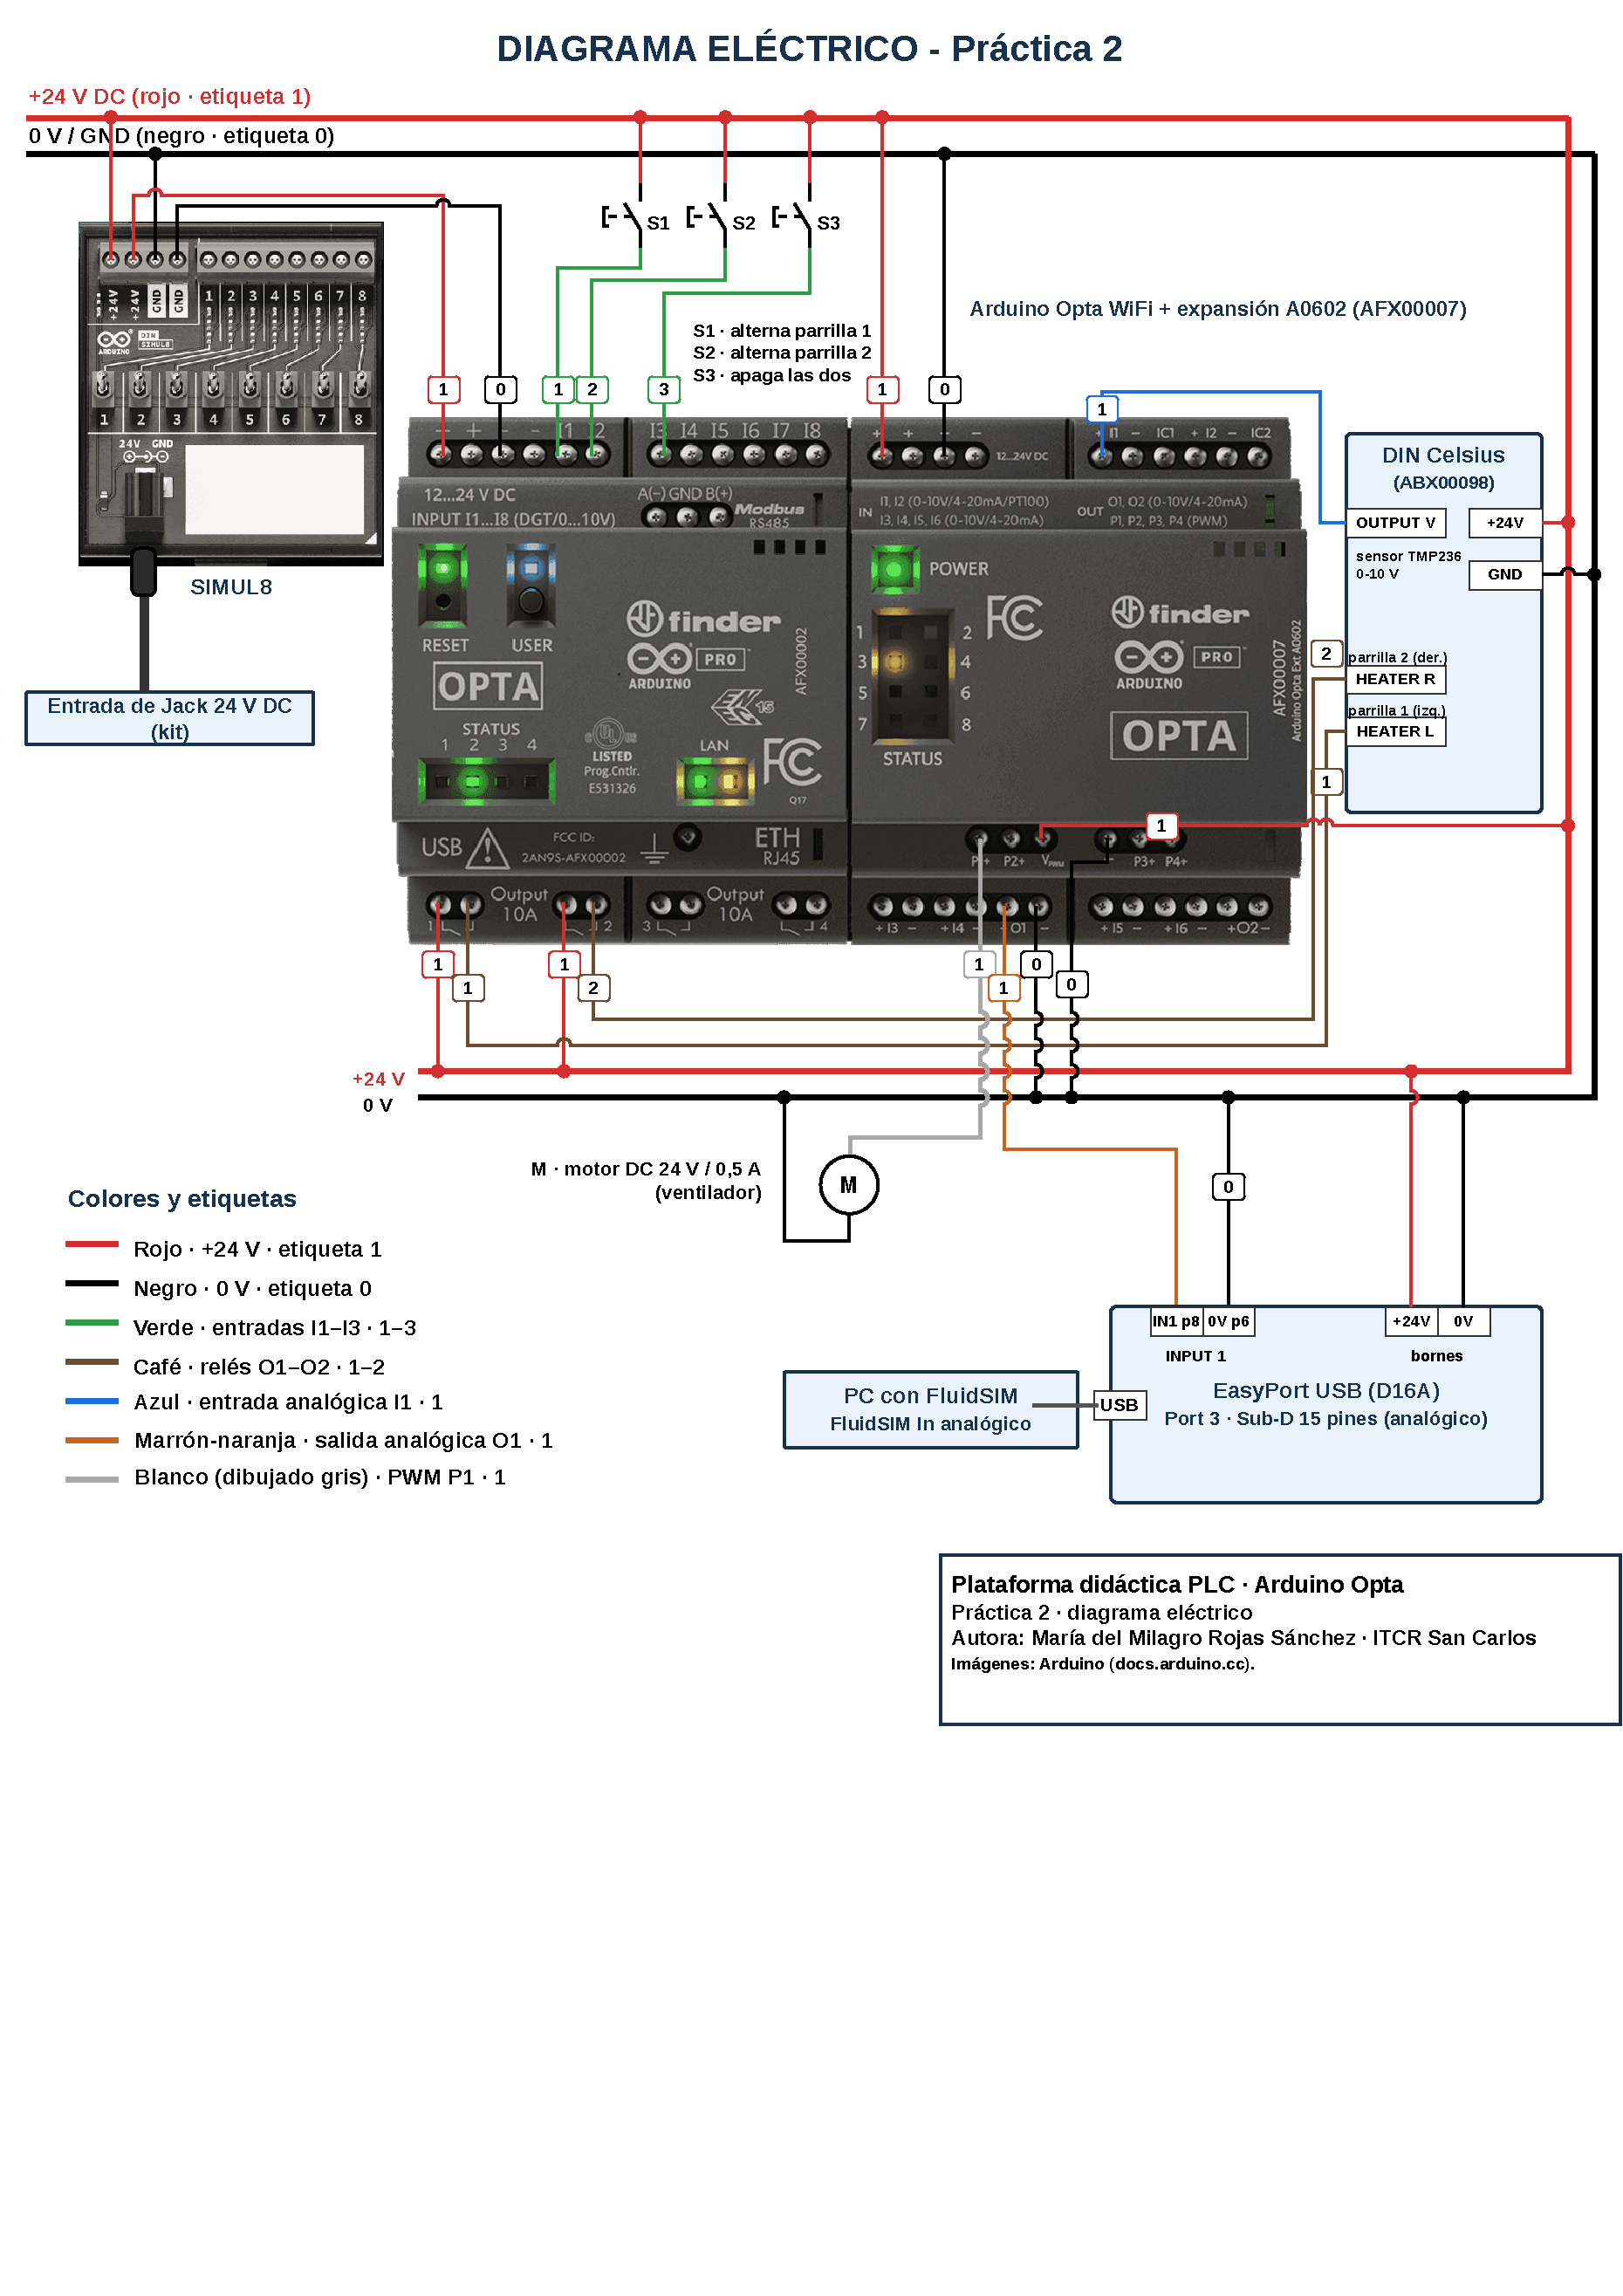
\includegraphics[width=\linewidth,trim=6 290 0 8,clip]{Diagrama_Electrico_Practica2.pdf}
    \caption{Diagrama eléctrico de las conexiones usadas en la
    Práctica~2. Fuente: Autora.}
    \label{fig:diagrama_p2}
\end{figure}

\subsubsection{Visualización de la señal analógica en el EasyPort}
\label{subsubsec:p2_pantalla}
La señal analógica de la práctica no pasa por FluidSIM: se lee
directamente en la pantalla del EasyPort. Con el cableado de la
figura~\ref{fig:diagrama_p2} (hilo amarillo de \texttt{O1} en el pin~8 del
conector analógico y tierra común en el pin~6), se procede así:

\begin{enumerate}
    \item Con el programa descargado y en ejecución, observar la pantalla
    del EasyPort. Muestra una tensión en voltios y, debajo, el canal que
    está leyendo.
    \item Pulsar las flechas \ui{$\uparrow$} y \ui{$\downarrow$} que están
    junto a la pantalla hasta que aparezca \ui{In Ch 0}, es decir, el
    canal~0 de las entradas.
    \item Comprobar que la tensión mostrada sigue a \texttt{PID\_OUT}: es
    \texttt{PID\_OUT}/10 en voltios, y cambia al encender o apagar las
    parrillas.
\end{enumerate}

El EasyPort numera sus entradas analógicas de 0 a 3 y sus salidas
analógicas de 0 a 1. La entrada~1 de la expansión (pin~8 del cable) es,
por tanto, el canal~0 de las entradas, que el programa EasyPort Web Bridge
nombra \ui{Uin 1}. Si la pantalla muestra otro canal, su valor no
corresponde a \texttt{O1}.

\begin{figure}[H]
    \centering
    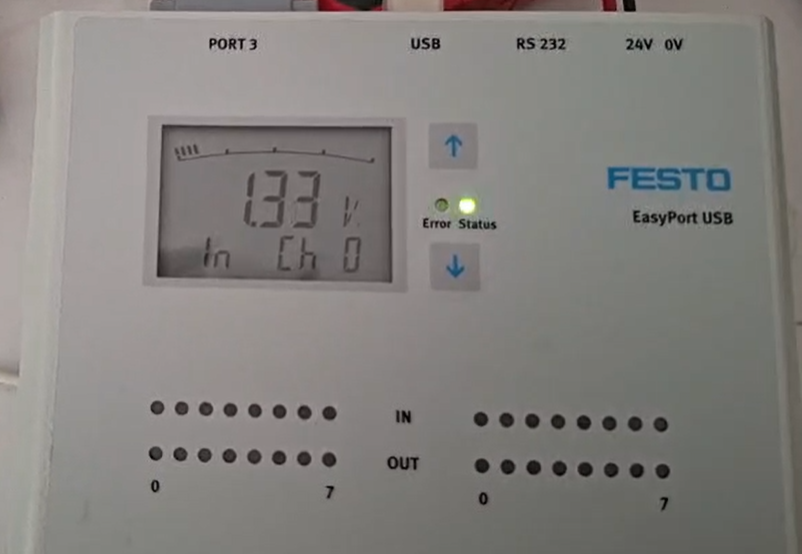
\includegraphics[width=0.6\linewidth]{Easy_Port_senalanalogica.png}
    \caption{Pantalla del EasyPort leyendo la salida \texttt{O1} de la
    expansión en el canal~0 de las entradas (\ui{In Ch 0}): 1,33~V en el
    momento de la captura. Fuente: Autora.}
    \label{fig:p2_easyport_pantalla}
\end{figure}

% =================================================================
\appendix
\renewcommand{\thesection}{Apéndice \Alph{section}}
% =================================================================

\section{Circuito completo de la Práctica 1}
\label{app:circuito}

\begin{figure}[H]
    \centering
    \rotatebox{90}{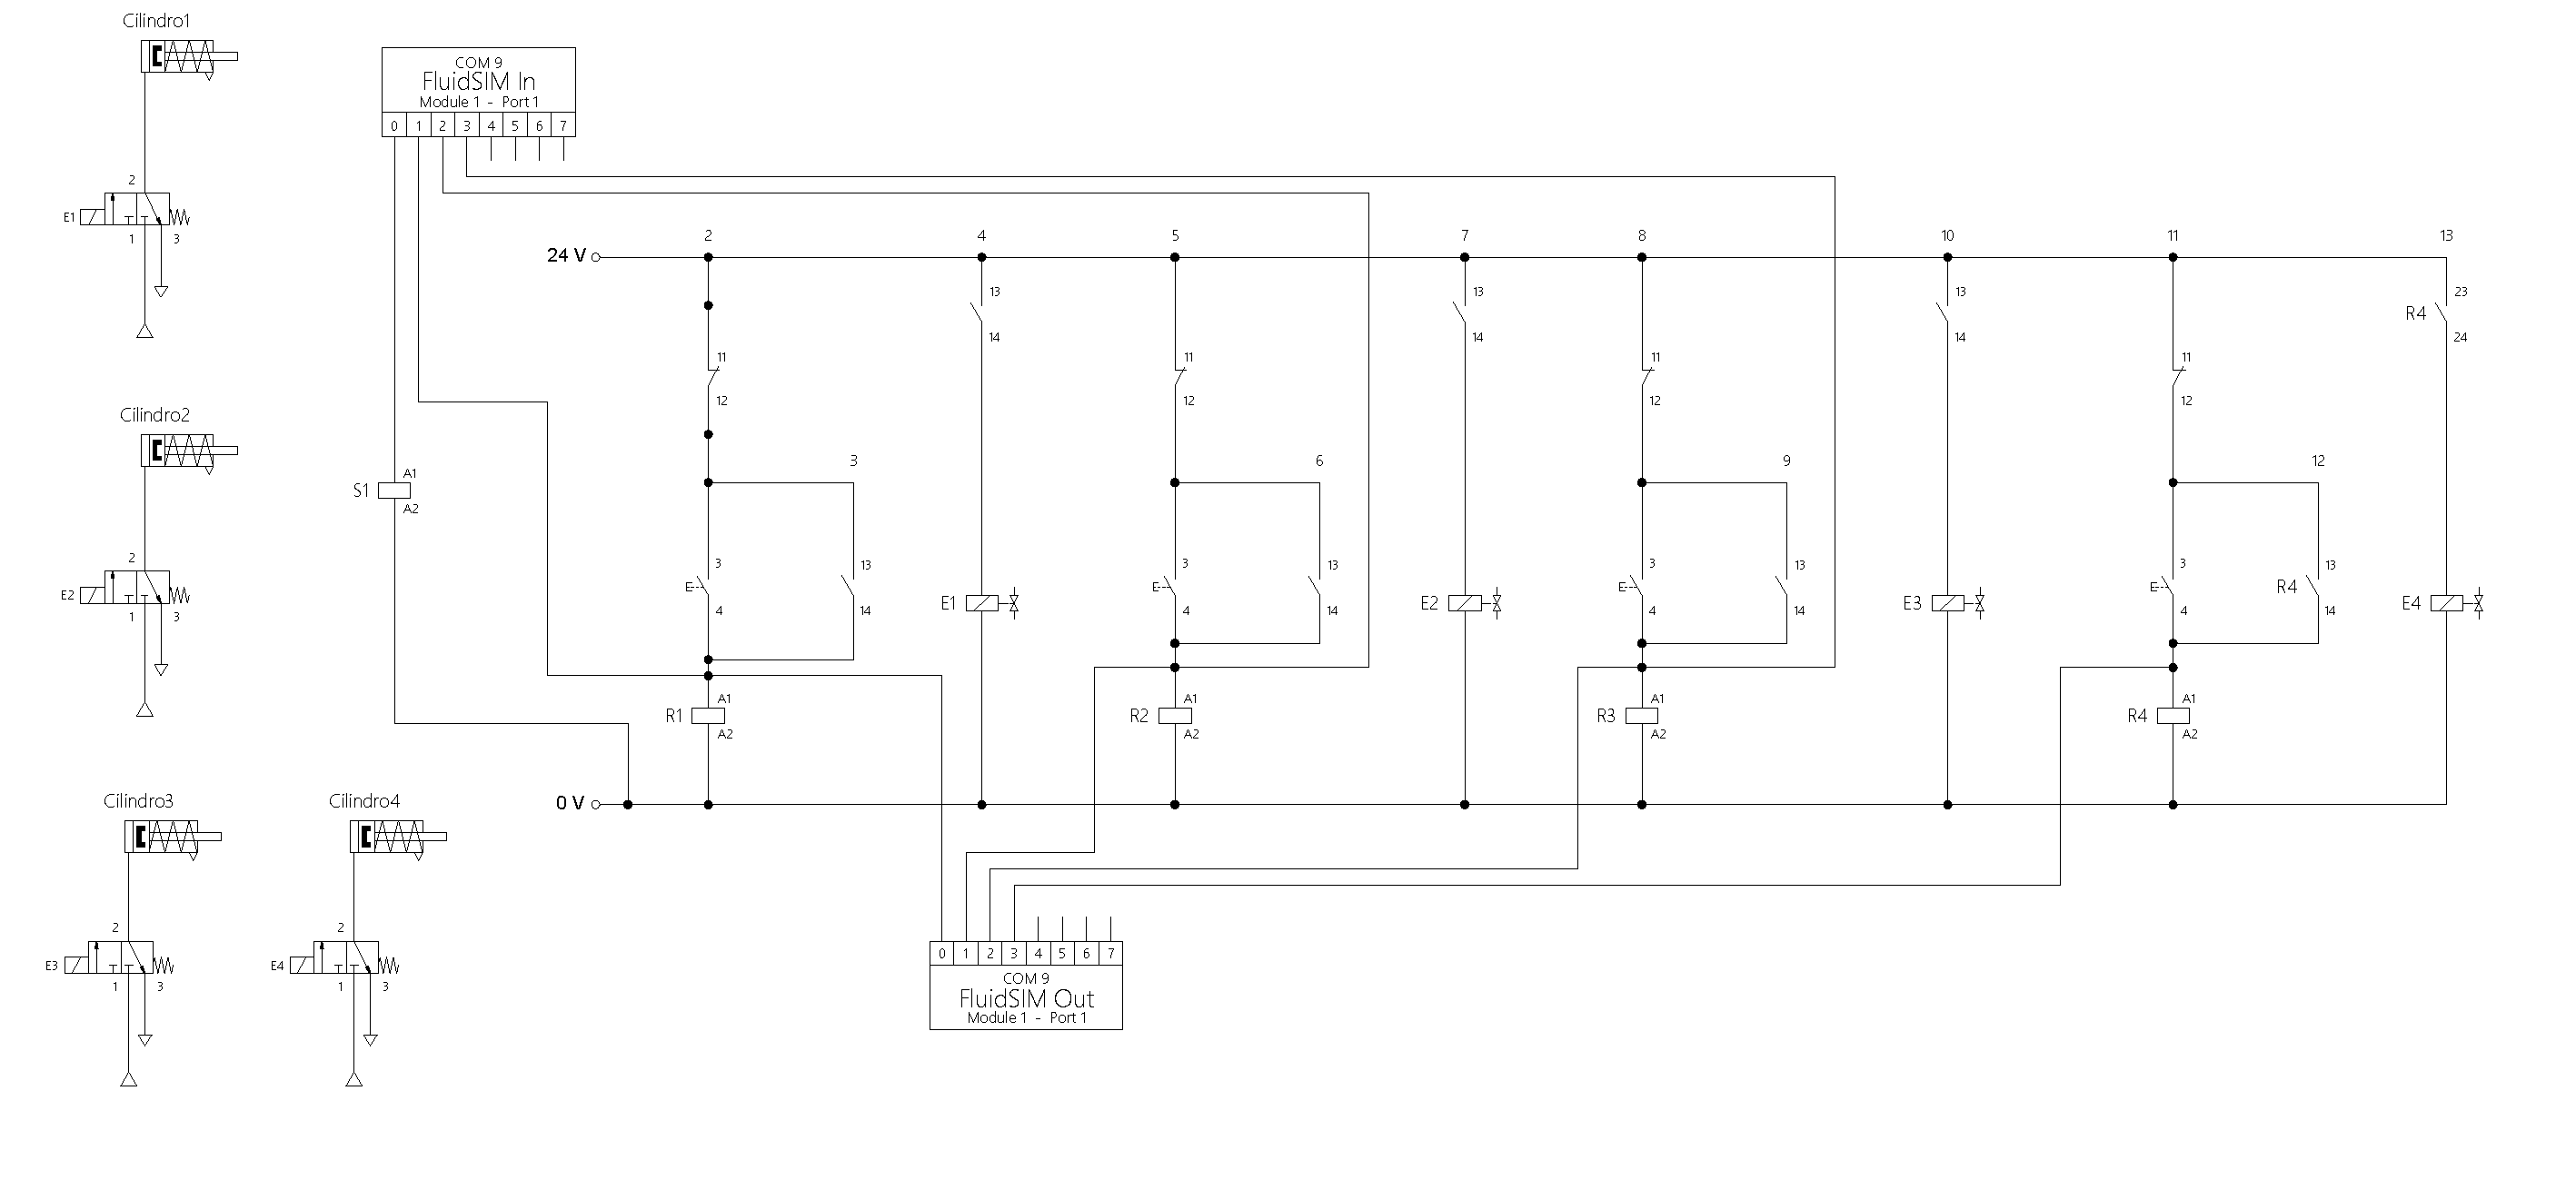
\includegraphics[width=0.8\textheight, trim=20 45 45 3, clip]{Ejercicio1_completo.pdf}}
    \caption{Circuito completo de la Práctica~1 en FluidSIM, a página
    completa.}
    \label{fig:fs_completo_grande}
\end{figure}

\clearpage
\section{Actualización del firmware de la expansión A0602}
\label{app:firmware}

Este apéndice describe cómo se actualizó la expansión de la versión 0.1.4
a la 0.1.14 (sección~\ref{subsubsec:p2_hw}). Se hace con Arduino IDE, no
con el PLC IDE.

\begin{enumerate}
    \item Con la expansión conectada al Opta y ambos alimentados, abrir
    Arduino IDE (la autora usó la versión 2.3.10).
    \item En \menu{Tools}{Board} $\to$ \ui{Boards Manager}, instalar el
    paquete \ui{Arduino Mbed OS Opta Boards} (\texttt{arduino:mbed\_opta},
    versión 4.6.0 en este caso). En \ui{Library Manager}, instalar la
    librería \ui{Arduino\_Opta\_Blueprint}.
    \item Seleccionar la placa \ui{Opta} y su puerto COM
    (figura~\ref{fig:p2_fw_sketch}).
    \item Abrir el ejemplo \texttt{updateExpansionFw}, que está en los
    ejemplos de la librería: \menu{File}{Examples} $\to$
    \ui{Arduino\_Opta\_Blueprint} $\to$
    \texttt{updateExpansionFw}~\cite{optaanalogtut}.
    \item Abrir el \ui{Serial Monitor} antes de que termine de cargar el
    sketch, cargarlo con \ui{Upload} y esperar los mensajes. El sketch
    informa las versiones disponibles (0.1.14 para la expansión analógica)
    y la versión instalada.
    \item Responder \texttt{Y} a \emph{Is the number of detected expansions
    correct?} y de nuevo \texttt{Y} a \emph{Expansion 0 will be now
    updated\ldots{} Proceed?}. Al terminar aparece \emph{UPDATE successfully
    performed} (figura~\ref{fig:p2_fw_serial}).
    \item En el PLC IDE, volver a descargar el \emph{runtime} al Opta y
    reconectar.
\end{enumerate}

\begin{figure}[H]
    \centering
    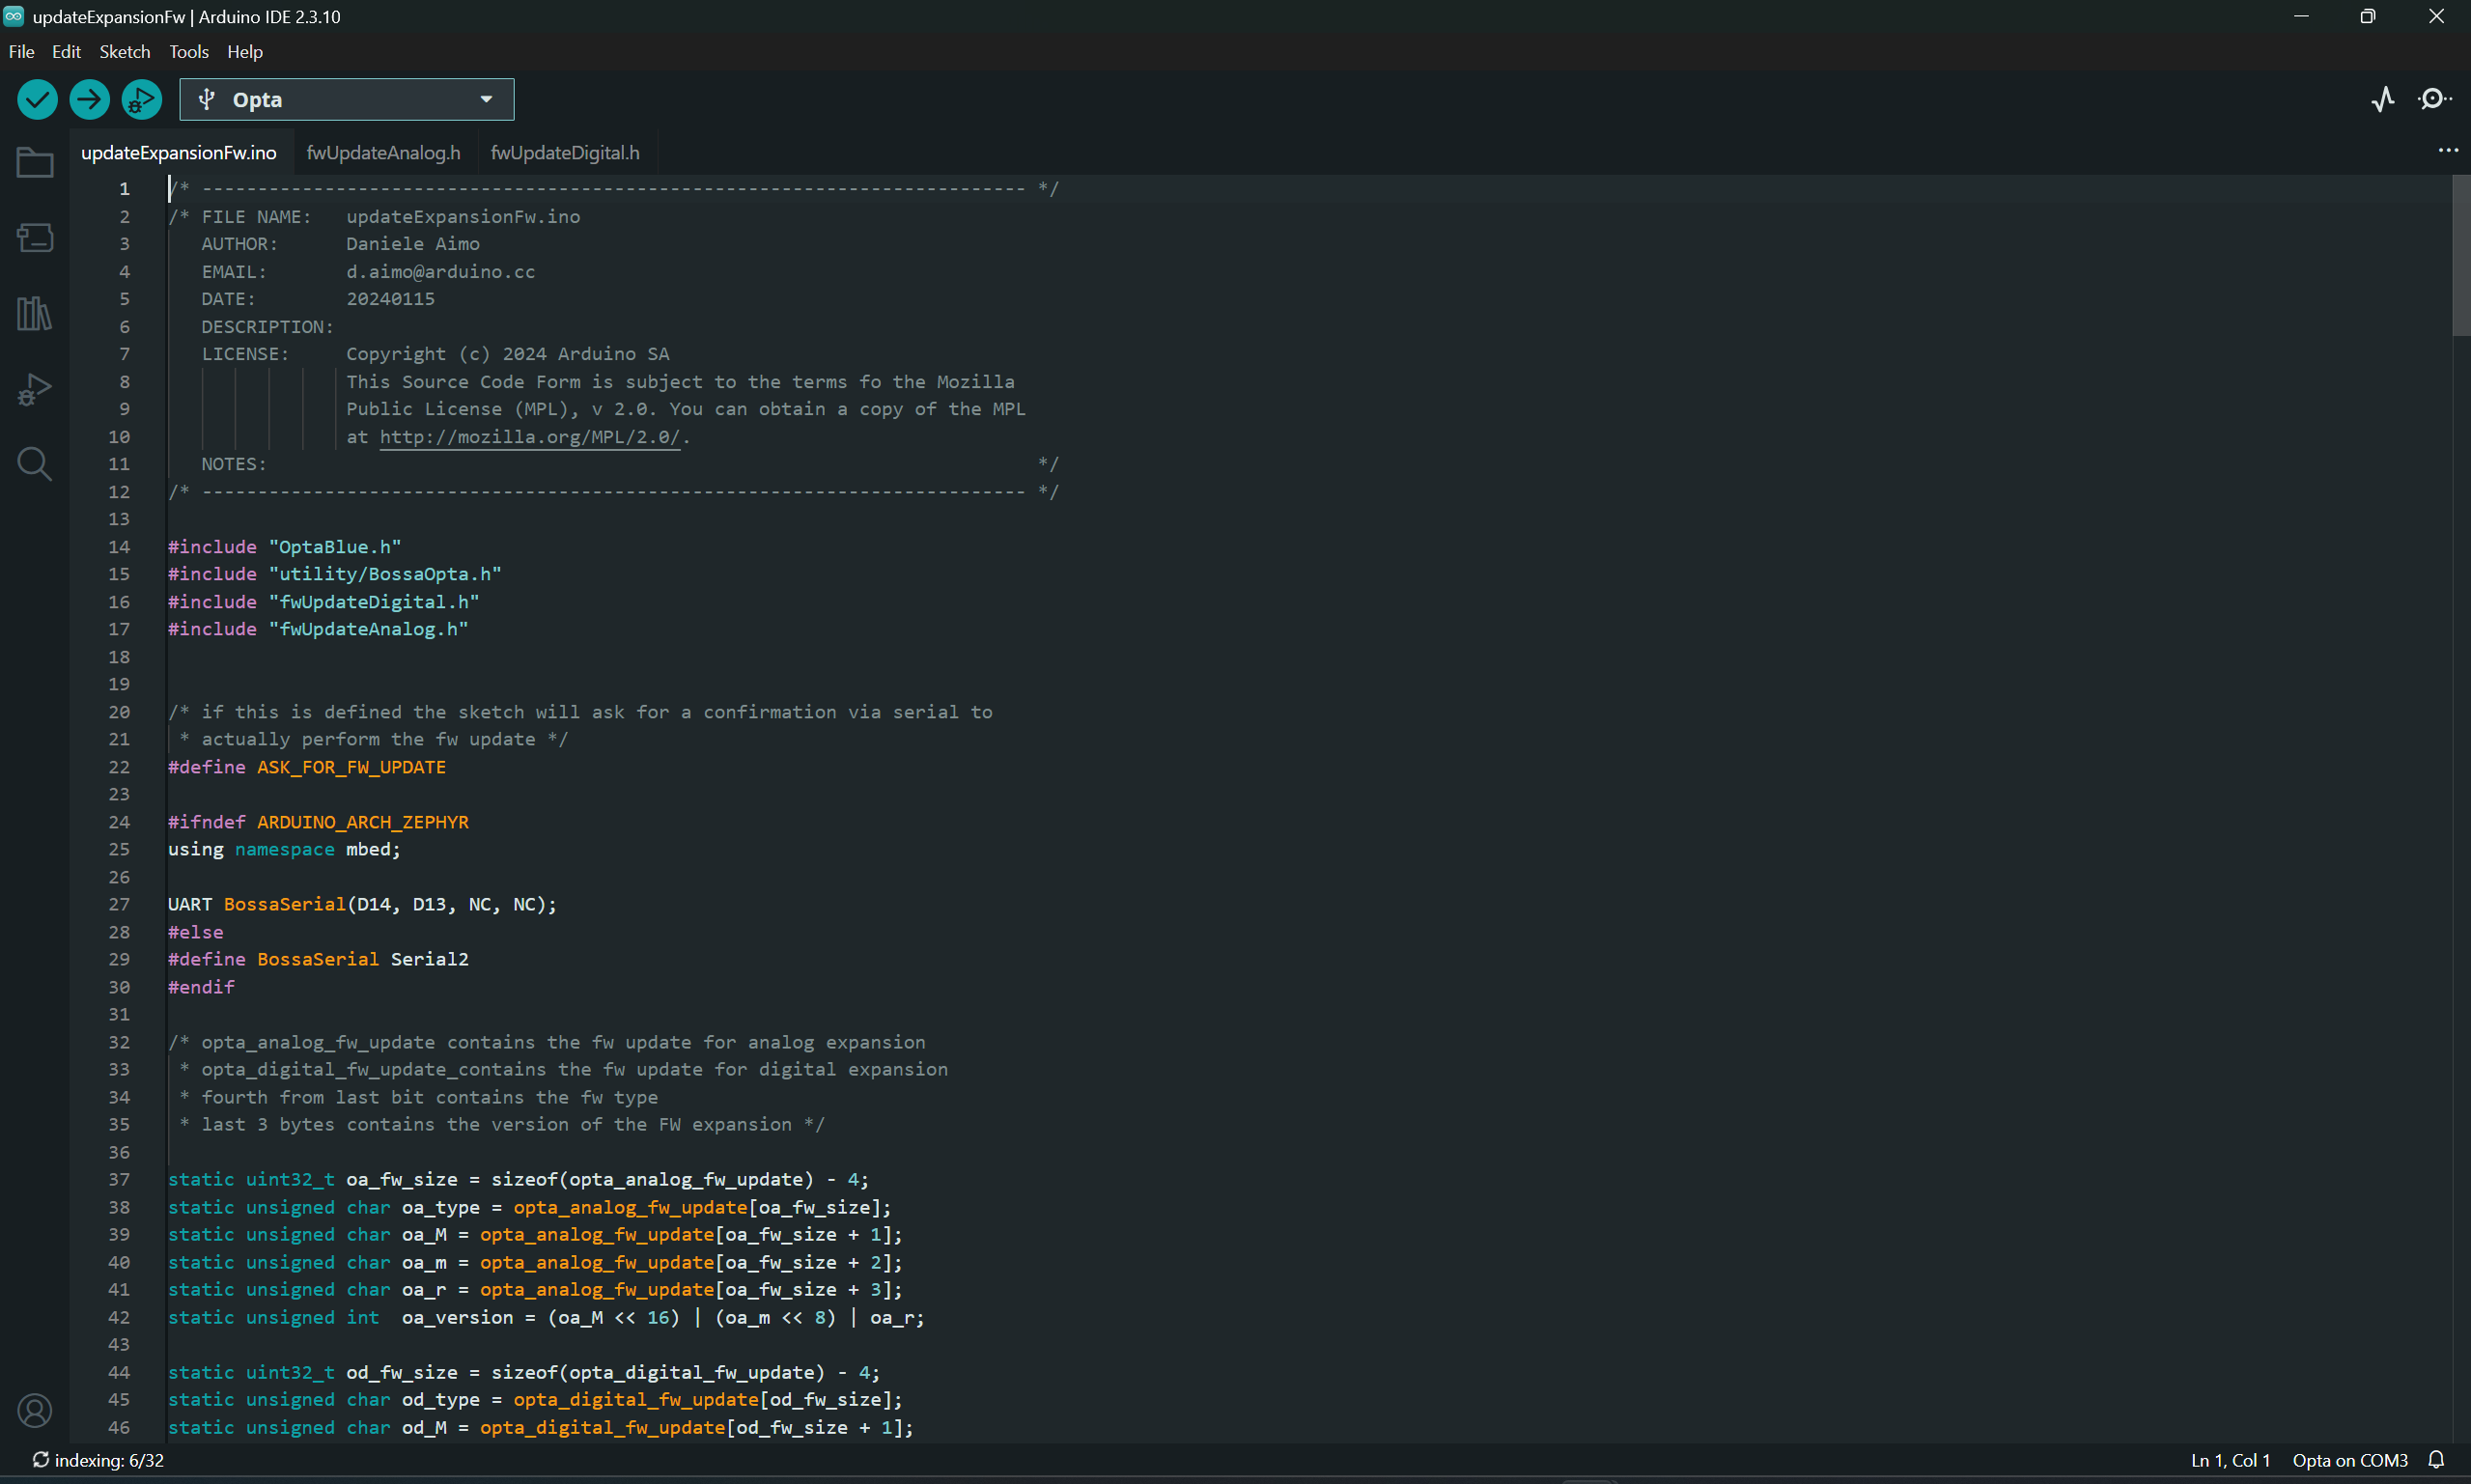
\includegraphics[width=0.85\linewidth]{p2_firmware_sketch.png}
    \caption{Sketch \texttt{updateExpansionFw} abierto en Arduino IDE con
    la placa \ui{Opta} seleccionada.}
    \label{fig:p2_fw_sketch}
\end{figure}

\begin{figure}[H]
    \centering
    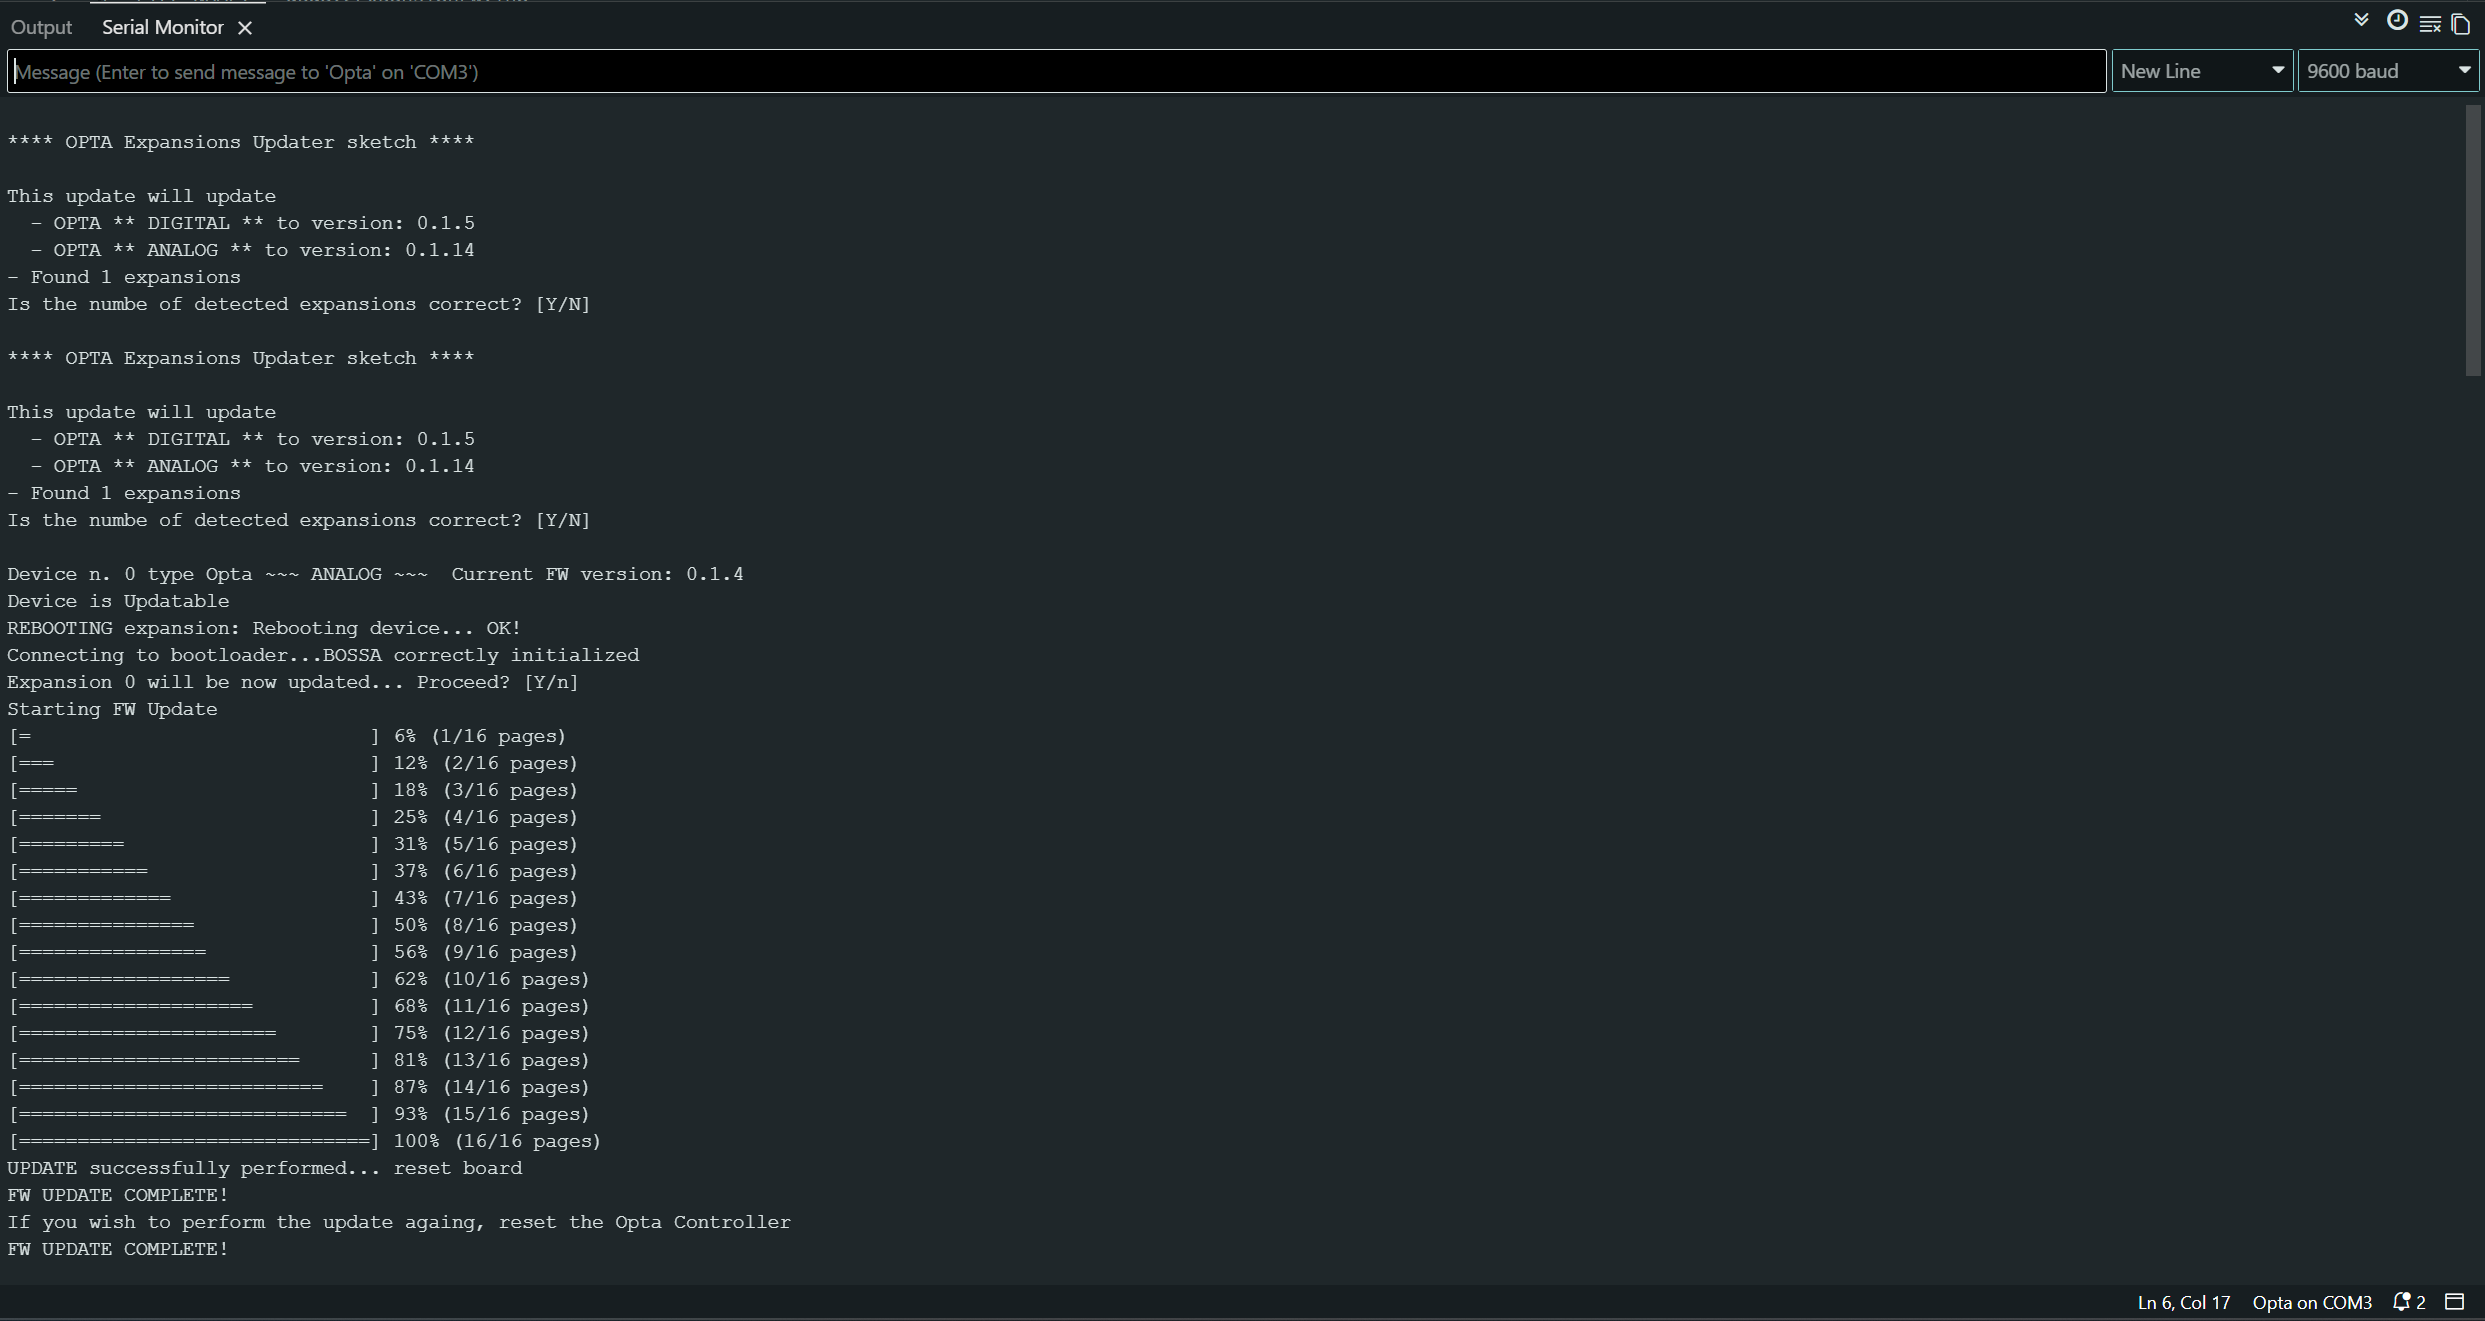
\includegraphics[width=\linewidth]{p2_firmware_serial.png}
    \caption{\ui{Serial Monitor}: la expansión pasa de la versión 0.1.4 a
    la 0.1.14.}
    \label{fig:p2_fw_serial}
\end{figure}

\begin{advertencia}
Si \ui{Upload} falla con \texttt{No DFU capable USB device available}
(código de salida 74), cerrar cualquier programa que use el puerto del Opta
(\ui{Serial Monitor}, PLC IDE) y poner el Opta en modo DFU con doble
pulsación del botón de reinicio; después repetir la carga. En la prueba de
la autora, el segundo intento cargó correctamente.
\end{advertencia}

% =================================================================
\begin{thebibliography}{9}

\bibitem{plcintro}
Arduino, ``Programming Introduction with Arduino PLC IDE,'' \emph{Arduino
Documentation}. [En línea]. Disponible en:
\url{https://docs.arduino.cc/software/plc-ide/tutorials/plc-programming-introduction/}.

\bibitem{optaanalogtut}
Arduino, ``Opta Analog Expansion Usage with the PLC IDE,'' \emph{Arduino
Documentation}. [En línea]. Disponible en:
\url{https://docs.arduino.cc/software/plc-ide/tutorials/opta-analog-expansion-plc-ide/}.

\bibitem{fluidsim}
Festo, ``Simulation software FluidSIM,'' \emph{Festo}. [En línea]. Disponible en:
\url{https://www.festo.com/us/en/e/technical-education/digital-learning/virtual-simulation-and-modeling/fluidsim-id_1663056}.

\bibitem{fluidsimlib}
Art Systems, ``FluidSIM 6 Component Library,'' \emph{Art Systems Software}.
[En línea]. Disponible en:
\url{https://www.art-systems.de/www/site/en/fluidsim/components.html}.

\bibitem{easyport}
Festo Didactic SE, \emph{EasyPort USB: Manual}, ref.\ 721876, ed.\ 10/2011,
Denkendorf, Alemania, 2011.

\bibitem{syslinkcable}
Festo Didactic GmbH \& Co., \emph{Cable de E/S con conector SysLink y
terminales abiertos: hoja de datos}, ref.\ 380156, ed.\ 04/2000.

\bibitem{syslinkweb}
Festo, ``Cable de datos de I/O con conector SysLink en un lado,'' \emph{Festo
México}. [En línea]. Disponible en:
\url{https://www.festo.com/mx/es/p/cable-de-datos-de-i-o-con-conector-syslink-en-un-lado-id_PROD_DID_167122}.

\bibitem{celsius}
Arduino, \emph{Arduino DIN Celsius: User Manual}, SKU ABX00098. [En
línea]. Disponible en:
\url{https://docs.arduino.cc/resources/datasheets/ABX00098-datasheet.pdf}.

\bibitem{a0602}
Arduino, \emph{Arduino Opta Analog Expansion: User Manual}, SKU
AFX00007. [En línea]. Disponible en:
\url{https://docs.arduino.cc/resources/datasheets/AFX00007-datasheet.pdf}.

\end{thebibliography}

\end{document}
